\documentclass[print]{tudelft-report}

\usepackage[framed,numbered,autolinebreaks,useliterate]{mcode} % To input .m files
% Input matlab code: \lstinputlisting{matlab_files/propSim.M}
\usepackage[justification=centering]{caption}	% Center captures under figures
\usepackage{epstopdf}							% Add matlab figures as .eps files
\usepackage{cleveref}							% Reference to multiple figures
\usepackage{gensymb}

\usepackage{subcaption}

%\usepackage{mathabx}

\usepackage[T1]{fontenc}
\usepackage{enumitem}

\usepackage{placeins}						% For the figures in the appendix

%Nomenclature
\usepackage{nomencl}
\makenomenclature
% Add nomenclatures as \nomenclature{$a$}{The number of angels per unit area}
% makeindex beamformer_thesis.nlo -s nomencl.ist -o beamformer_thesis.nls

% For rotated tables
\usepackage{rotating}	
\usepackage{adjustbox}
\usepackage{graphicx}
\usepackage{multirow}

\newcommand{\matlab}{\textsc{Matlab} } %fancy Matlab commando
\newcommand{\norm}[1]{\left\lVert#1\right\rVert}
\newcommand{\argmin}{\arg\!\min}

\graphicspath{{images/}}

\begin{document}

%% Use Roman numerals for the page numbers of the title pages and table of
%% contents.
\frontmatter

\title[\today]{Acoustic Enhancement via Beamforming using Smartphones}

\author{N. van Wijngaarden 4063899\\E. H. Wouters 4095421}

\affiliation{Delft University of Technology}

%\coverimage{cover.jpg}
\makecover

%% Include an optional title page.
%\begin{titlepage}

\begin{center}

%% Insert the TU Delft logo at the bottom of the page.
\begin{tikzpicture}[remember picture,overlay]
    \node at (current page.south)[anchor=south,inner sep=0pt]{
        
\includegraphics{cover/logo}
    };
\end{tikzpicture}

%% Extra whitespace at the top.
\vspace*{2\bigskipamount}

%% Print the title in cyan.
{\makeatletter
\titlestyle\color{tudelft-cyan}\Huge\@title
\makeatother}

%% Print the optional subtitle in black.
{\makeatletter
\ifx\@subtitle\undefined\else
    \bigskip
    \titlefont\titleshape\LARGE\@subtitle
\fi
\makeatother}

\bigskip
\bigskip

by
%door

\bigskip
\bigskip

%% Print the name of the author.
{\makeatletter
\titlefont\Large\bfseries\@author
\makeatother}

\vfill

in partial fulfillment of the requirements for the degree of
%in overeenstemming met de vereisten voor het verkrijgen van de graad van

\bigskip
\bigskip

{\bfseries Master of Science}

in Applied Physics

\bigskip
\bigskip

at the Delft University of Technology,
%aan de Technische Universiteit Delft,

to be defended publicly on Tuesday January 1, 2013 at 10:00 AM.
%in het openbaar de verdedigen op dinsdag 1 januari om 10:00 uur.

\vfill

\begin{tabular}{lll}
%% Add additional information here, per faculty requirements, e.g
%    Student number: & 1234567 \\
%    Project duration: & \multicolumn{2}{l}{March 1, 2012 -- January 1, 2013} \\
    Supervisor: & Prof.\ dr.\ ir.\ A.\ Einstein \\
    Thesis committee:
        & Prof.\ dr.\ C.\ F.\ Xavier, & TU Delft \\
        & Dr.\ E.\ L.\ Brown, & TU Delft \\
        & Ir.\ M.\ Scott, & Acme Corporation
\end{tabular}

%% Only include the following lines if confidentiality is applicable.
\bigskip
\bigskip
\emph{This thesis is confidential and cannot be made public until December 31, 2013.}
%\emph{Op dit verslag is geheimhouding van toepassing tot en met 31 december 2013.}

\bigskip
\bigskip
An electronic version of this thesis is available at \url{http://repository.tudelft.nl/}.
%Een elektronische versie van dit verslag is beschikbaar op \url{http://repository.tudelft.nl/}.

\end{center}

\end{titlepage}



\chapter*{Preface}
\setheader{Preface}

Preface\ldots

\begin{flushright}
{\makeatletter\itshape
    \@author \\
    Delft, January 2013
\makeatother}
\end{flushright}



\tableofcontents

\printnomenclature[3cm]

\listoffigures	% create a list of figures
\listoftables	% create a list of tables

%% Use Arabic numerals for the page numbers of the chapters.
\mainmatter

\nomenclature{$\omega$}{Frequency [rad/s]}



\chapter*{Abstract}
\setheader{Abstract}

This thesis presents a comparison between two different beamforming algorithms, the delay-and-sum beamformer (DSB) and the minimum variance distortionless response (MVDR) beamformer using both objective and subjective metrics. Simulations and measurements have been performed on near-field scenarios with an ad-hoc microphone array. Microphones from multiple smartphones are used to record the audio. Smartphone microphones are designed to have a distinct directivty gain pattern. In this research, the MVDR algorithm is extended to compensate for these directivity responses. In simulated scenarios, without the directivities of the microphones, the average improvement in segmental signal to noise ratio is $5.3 dB$ for DSB and $11.9 dB$ for MVDR. In all the simulated scenarios, the MVDR beamforming algorithm outperforms the DSB algorithm. Results from measurements in an office room scenario only showed an improvement when applying the DSB algorithm. The results from measurements in the anechoic chamber at the TU Delft show $1.9 dB$ improvement for DSB and $2.8 dB$ for MVDR.
Compensating for the directivity in the implemented MVDR mainly added noise to the signal.
\chapter{Introduction}
\label{chap:introduction}

Companies and many other organizations depend more and more on teleconferencing as a means of communications. This is a viable solution that can reduce both cost and environmental impact of traveling long distances for meetings.
Commercially available, state of the art teleconferencing products usually require a controlled acoustic environment equipped with expensive hardware \cite{pentek2015}. However, nowadays it becomes increasingly more common to possess a smartphone. This brings forward the opportunity to use the microphones from multiple smartphones for audio conferencing. There are multiple aspects of audio quality to be considered in developing and designing a conference telephone system. A few examples are noise and reverberations \cite{vanveen1988}. These must be filtered from the microphone signals to avoid noise and echoes \cite{naylor2010speech}.

\section{Conference Calls}
\label{sec:intro_conference}
In a conference call, the interesting audio source is usually one person talking in a noisy room full of people. Therefore it is a challenge to enhance the sound from the source while suppressing the surrounding (noise) sources. Beamforming provides an effective and versatile means of spatial filtering \cite{vanveen1988}. This is useful when distinguishing desired signal components from noise and interference based on their locations.

\begin{figure}[b!]
    \centering
    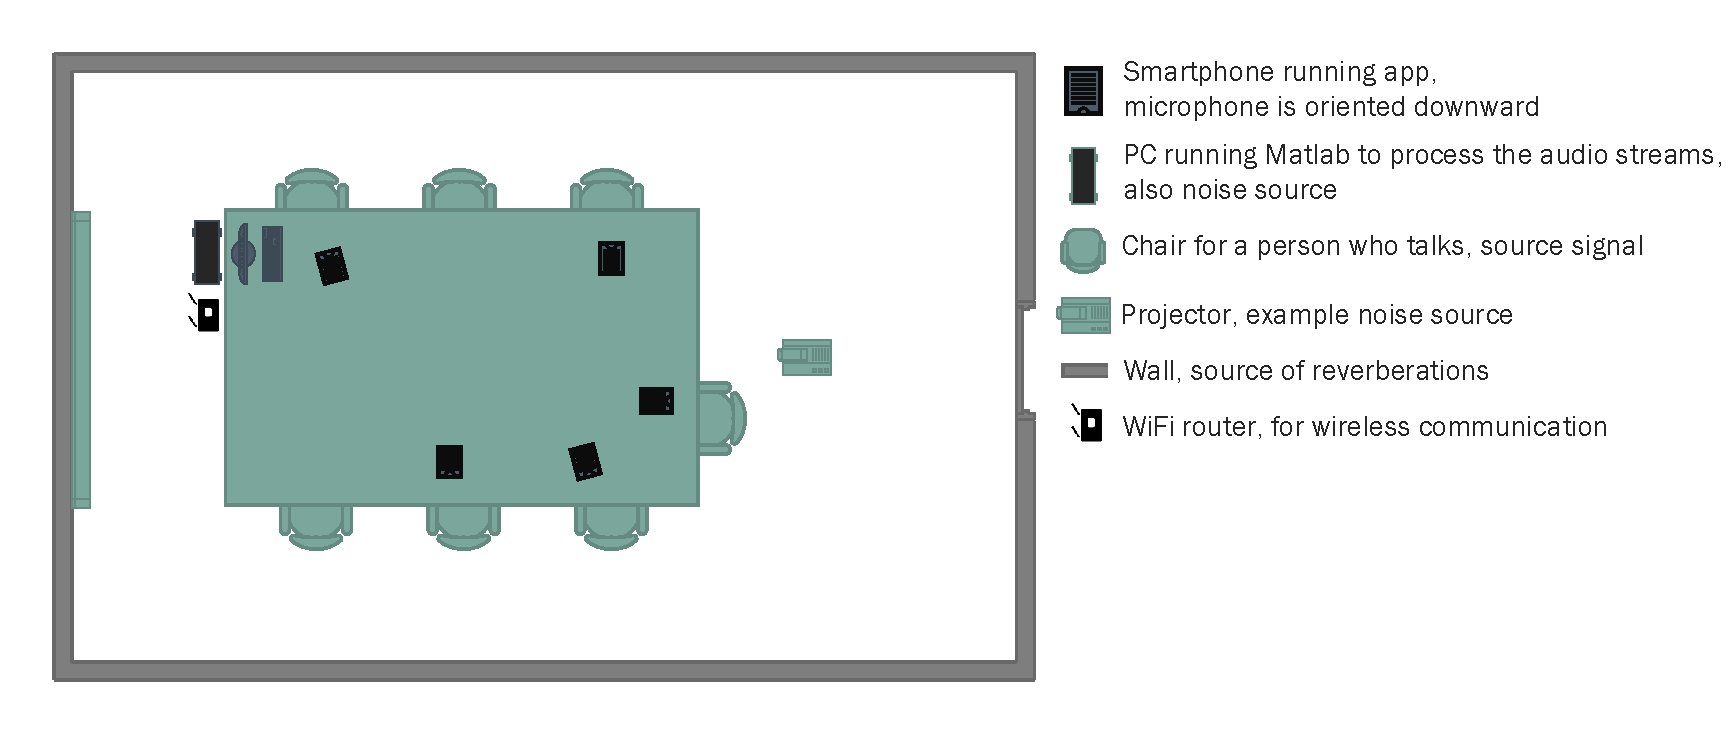
\includegraphics[width=15cm]{images/usage_scenario.pdf}
    \caption{An example usage scenario of the system in a conference call}
    \label{fig:SchemUsage}
\end{figure}

\section{Beamforming Algorithms}
\label{sec:intro_alg}
In this research, the delay-and sum beamformer and the minimum variance distortionless response (MVDR) beamformer are investigated. The MVDR beamformer is a very widely studied and used beamforming algorithm \citep{habetsspeech2010}, and is also used in commercially available arrays \citep{pentek2015}. The MVDR beamformer estimates the desired signal while minimizing the variance of the noise component of the formed estimate. The locations of the microphones are used to determine the direction of arrival (DOA). There are existing algorithms which can do source localization by using spectral estimation concepts and time-difference of arrival (TDOA) information \citep{brandstein2001}. Inaccuracies in the locations of the microphones degrade the performance of the MVDR beamformer significantly \citep{vanveen1988, ehrenberg2010}. Fortunately the microphone and source locations are known a priori in many cases \citep{himawan2011}. For this research perfect sound source localization (SSL) is assumed for both microphones and sources.

\section{Microphone Arrays}
\label{sec:intro_arrays}
Microphone arrays are a common way to improve the sound quality \citep{brandstein2001}. The diversity in the received signals is exploited by setting different gains to each microphone, depending on the location of the source and the interference. This is generally referred to as beamforming. Early designs were generally “fixed” beamformers like the delay-and-sum beamforming \cite{naylor2010speech}, adapting only to the location of the desired source. State of the art beamformers use statistical approaches which, in addition to the locations, also depend on assumptions about the acoustic composition of the signals \cite{gaubitch2014}. Iterative methods are also available which can adapt to specific noise and acoustic conditions \cite{griffiths1982,ba2007}. The latter methods have a considerably higher complexity \citep{kjellson2014sound}. \newline
A lot of research has been done into a class of algorithms known as robust MVDR beamformers \citep{ba2007,habets2010,martinez2015}. These algorithms improve upon previous work on two fronts, by extending the region where the source can be located and thus lowering the susceptibility to errors in the localization, and by including nonuniformity in the microphones directional response, known as microphone directivity.

\section{Microphone Directivity}
\label{sec:intro_directivity}
Real microphones may have distinct, directional responses. Experiments done by Ba et al. \citep{ba2007} show that the traditional MVDR beamforming algorithm and other existing algorithms perform well when omnidirectional microphones are used, but do not provide much enhancement when directional microphones are used. Simulations done by Martínez et al. \cite{gaubitch2014} show improvements of up to $6.1 dB$ in the segmental signal to noise ratio when using the measured directivity compared to assuming the microphones are omnidirectional \citep{martinez2015}. Aforementioned work used low cost smartphone microphones and the directivity pattern was measured in two dimensions. 
We will show in chapter \ref{chap:results} that including the directivity impulse response produced erratic results.
For the smartphones used in this work the directivities have been measured by our fellow team members \cite{BAP:RosalieTim}. This result is incorporated in the robust MVDR algorithm in section \ref{chap:design}. This has not been exploited much in the existing literature and in this thesis some of the challenges of implementing a realtime robust MVDR beamforming algorithm which adopts microphone directivity have been explored.

\section{Assessing Audio Quality}
\label{sec:intro_intelligibility}
In order to compare different beamformers, parameters and smartphone configurations an attempt has been made to write a realtime audio beamforming toolbox for \matlab which can interface with an Android app developed by our fellow team members \cite{BAP:RoySjoerd}. With this toolbox the impact of different aspects of beamforming on the quality estimators can be visualized in realtime. This enables rapid testing of different parameters and configurations. There are different quality estimators to analyze the performance of a beamformer. There are power related measures and intelligibility measures. Intelligibility is the degree to which speech can be understood and hence the corresponding measures can be evaluated to determine the effect of the beamformers on the speech intelligibility of the signals \cite{gerrits2014evaluation}.

\section{Reading Guide}
\label{sec:intro_reading}
This thesis is organized as follows. The last section (\ref{sec:intro_req}) of this introduction contains a schedule of requirements which was made at the start of the project. In chapter \ref{chap:problem}, the problem definition and observation model of this research will be defined. The research that has already been conducted in this topic will be discussed in section \ref{chap:related}. The design process is described in section \ref{chap:design}. The results are presented in section \ref{chap:results}. A discussion on these results is given in section \ref{chap:discussion}. A conclusion is drawn in section \ref{chap:conclusion}. Detailed results from the data analysis can be found in appendix \ref{app:res}.


\section{Requirements}
\label{sec:intro_req}
%\subsection{Introduction}
The aim of the system that will be implemented is to record audio, using smartphones, in a room with multiple audio sources and compare the performance of different beamforming algorithms. This comparison is done by showing different quantitative analyses related to a beamforming algorithm in a way that a user can compare the differences at a glance.

\subsection{Requirements concerning the intended use}
\begin{enumerate}
\item The system must have the possibility to either select local audio files for simulation or post-processing, or connect to smartphones for realtime calculations.
\item The noise has to be suppressed while maintaining the sound level of the source.
\item The noise source can be located anywhere, except at the source location.
\item The system must be able to switch between different types of beamformers.
\item The system must be able to compare the received audio from one of the smartphones before and after applying one of the beamformers.
\item The system must calculate and compare intelligibility metrics to determine the quality of the output for speech purposes.
\item The system must calculate and compare power related metrics to determine the quality of the output.
\item The system must be able record sound using smartphones.
\item The system must be able to play the beamformed audio over the speakers.
\item The system must be able to connect to the smartphones and handle the streaming data.
\item All of the requirements should be achieved in situations where the near-field assumptions hold.
\end{enumerate}

%After finishing recording, it has to be possible to save the output of each of the beamformers. 
%The system must be able to save the output of each of the beamformers.

% Consider following requirements
% It should be possible to filter at least 1 punctuated noise source by decreasing its power by at least 10 dB.

% It should be possible to aim a beam with a ’1’ response in an indicated target direction.

% Filtering has to be possible on the spectrum used for human speech, i.e. 300-3400 Hz.

\subsection{Requirements concerning the system}
\begin{enumerate}
\item The beamforming algorithms can be applied to real-time audio signals or previously recorded files.
\item For realtime beamforming, the communications between matlab and the smartphones will be monitored.
 For each smartphone individually the location, orientation and if the smartphone is placed face up or face down on the table can be entered.
\item Recording can be started and stopped by pressing a start/stop button.
\item The different beamformers can be turned on or of by ticking the corresponding box.
\item Each of the different kinds of intelligibility and power related calculations can be selected or deselected.
\item While recording, the location(s) of the source(s) and microphone(s) will be plotted on the screen in 3D.
\item After recording, the relevant data can be saved to an audio file, including sufficient data labels such as locations to make post-processing possible.
\item In the non realtime case, the user will be able to select a time frame which will be beamformed and over which the intelligibility and power related measures will be computed.
\end{enumerate}
\chapter{Problem Definition}
\label{chap:problem}

\section{Array Signal Processing}
\label{sec:problem_array}
In general array signal processing is concerned with three tasks: detection of noise signals, estimation of the direction of arrival and beamforming. The locations of the microphones and speakers in the room are usually stationary. These locations hold valuable information which can be used when processing the audio signal. An elaborate method to process this signal is beamforming \cite{lui2010}. This is a statistical method to estimate parameters, which is further complicated by the spatial dimensions of the array. Krim and Viberg formulate the problem of sensor array processing as: \textit{"\dots the estimation of parameters by fusing temporal and spatial information, captured via sampling a wavefield with a set of judiciously placed antenna sensors."} \cite{krim1996}.

\section{Ad-hoc}
\label{sec:problem_ad-hoc}
The techniques used in beamforming are not strictly valid for microphone sensor arrays, but may also hold for other types of sensor arrays. The geometry, size and number of the sensor array can vary. The geometry of the sensor array may vary from linear, circular or spherical to arbitrary geometries. This research focuses on the last type of geometry, which we will call an \textit{ad-hoc microphone array}.

\section{Near-field}
\label{sec:problem_near-field}
There is an important distinction to be made with respect to the dimensions of the array or \textit{aperture} size. There exist different methods for \textit{far-field} and \textit{near-field} beamforming. In far-field one can assume that the wave field originates from a distance far greater than the dimensions of the array, which leads to the assumption that the wave field has a flat wave front. This means that the Direction Of Arrival (DOA) is the same for every sensor in the array. In near-field beamforming the distance from the source of the wave field to the array is comparable in magnitude to the dimensions of the array. This means that every sensor gets a different DOA and amplitude of the signal. \newline
An often used rule to decide whether the far-field approximation is valid is $r = 2L^2/\lambda$ where $r$ the distance from the microphone array to the source, $L$ the largest array dimension and $\lambda$ the operating wavelength \cite{kennedy1998}. In the scenario outlined in section {\ref{chap:introduction}} the dimensions of the microphone array are large with respect to the distance between the array and the source. Therefore, according to the earlier mentioned rule, we can assume that the sources of interest are in the near-field region \cite{gaubitch2014}. In addition, the positioning of the microphones is arbitrary, but known. As such, the main focus for our implementation will be near-field beamforming with ad-hoc microphone arrays. 

\nomenclature{$L$}{Largest array dimension [m]}
\nomenclature{$\lambda$}{Wavelength [m]}

\section{Broadband}
\label{sec:problem_broadband}
There is one more distinction to be made in type of the beamformer. There are different design techniques for broadband and narrowband beamformers. In speech communication applications broadband design implies design over several octaves. In order to use the processed signals for speech communications, the beamformers have to perform well over the frequency band from $300 Hz$ to $3400 Hz$ \cite{ituspeechfreq2011}.

\section{Observation Model}
\label{sec:observation}

Figure \ref{fig:observation} shows a representation of a room with some $x$, $y$ and $z$ dimensions and $M$ microphones. An acoustic source signal $s(t)$ originating from a position $\textbf{p}_{src}^{j}$ will propagate through the room and reach all the microphones positioned at $\textbf{p}_{mic}^{i}$. At a time $t$ the sampled microphone signal for each microphone consists of delayed and attenuated versions of the source signal $a_{i}s(t-\tau_{i})$ with undesired signal components $v_{i}(t)$ added to it. The acoustic transfer function (ATF) of the room is denoted by $h_{i}(t)$. For this research the ATF of an anechoic room is assumed unless otherwise specified:

\nomenclature{$M$}{Number of microphones}
\nomenclature{$\textbf{p}$}{Position vector in space [m]}
\nomenclature{$t$}{Time [s]}
\nomenclature{$s(t)$}{Acoustic source signal in the time domain}
\nomenclature{$a$}{Attenuation coefficient [$\text{m}^{-1}$]}
\nomenclature{$\tau$}{Delay of a signal [s]}
\nomenclature{$v(t)$}{Undesired signal components in the time domain}
\nomenclature{$h(t)$}{Acoustic transfer function in the time domain}

\begin{equation}
\label{eq:ATF}
H_{i,j}(\omega) = \frac{\exp(-j\omega \dfrac{r_{i,j}}{c})}{4\pi r_{i,j}}
\end{equation}

\nomenclature{$H(\omega)$}{Acoustic transfer function in the frequency domain}
\nomenclature{$r$}{Distance between source and mic [m]}
\nomenclature{$c$}{Speed of sound [m/s]}

with
\begin{equation}
r_{i,j} = \norm{\textbf{p}_{mic}^{i}-\textbf{p}_{src}^{j}}
\end{equation}

where $c$ is the speed of sound; $\textbf{p}$ is the position vector in space. In many cases there will be only one source of interest, so the $j$ index may be omitted.
The ATF is represented in the Fourier domain. The positions and orientations of the microphones and sources are assumed to be known. The ATF describes the set of all the propagation paths from a source to a microphone and hence the convolution between the sound coming from the source and the impulse response results in the sound recorded by the microphones. If the microphone has nonuniform directivity gain the room ATF is convolved over time with the directivity pattern of the microphone $g(t,\theta,\phi)$:

\begin{equation}
\label{eq:look}
d_{i}(t,\theta,\phi) = h_i(t) \ast g_i(t,\theta,\phi)
\end{equation}

\nomenclature{$d(t,\theta,\phi)$}{Array response vector [s]}
\nomenclature{$g(t,\theta,\phi)$}{Directivity pattern of a microphone in the time domain}
\nomenclature{$\theta$}{Azimuth [$\degree$]}
\nomenclature{$\phi$}{Elevation [$\degree$]}

where "$\ast$" denotes the convolution; $g_i(t,\theta,\phi)$ is the directivity impulse response \cite{BAP:RosalieTim} of the specific microphone, $\theta$ and $\phi$ are the azimuth and elevation angles between the source and the respective microphone. This directivity pattern was measured in the anechoic chamber of the Faculty of Applied Sciences at TU Delft for the smartphones used in this research. For omnidirectional microphones a Kronecker delta can be used for $g_i$, or it can simply be omitted. We can combine the attenuation and delay for all microphones into one vector:

\begin{equation}
\textbf{d}(\omega,\theta,\phi) = [A_{1}(\omega,\theta,\phi)e^{-j\omega\tau_{1}},A_{2}(\omega,\theta,\phi)e^{-j\omega\tau_{2}},...,A_{M}(\omega,\theta,\phi)e^{-j\omega\tau_{M}}]^{T}
\end{equation}

\nomenclature{$\textbf{d}(\omega,\theta,\phi)$}{Look vector of the array}
\nomenclature{$y(t)$}{Received audio signal by a microphone in the time domain}

where $\textbf{a}^{T}$ denotes the transpose of the vector $\textbf{a}$. The vector $\textbf{d}$ is called the \textit{look vector} of the array. $A_{i}$ is the combined attenuation factor due to the ATF and the directivity $\tau_{i}$ is the combined delay due to the ATF and the directivity.
\\
We model the received signals ${y}_{i}(t),i \in \left\{ {1,...,M}\right\}$ at each sensor using equation \ref{eq:look} as:

\begin{equation}
\label{eq:observationtime}
{y}_{i}(t) = a_{i}s(t-\tau_{i}) \ast g_i(t,\theta,\phi) + v_i(t)
\end{equation}

where $v_i(t)$ denotes the undesired signal components which consist of noise and reverberations (the dotted lines in figure \ref{fig:observation}) and signals from interfering sources. $a_i$ is the attenuation factor due to the ATF. The delay between when the signal is at the reference microphone and the $i^{th}$ microphone is $\tau_{i} = \norm{\textbf{p}_{mic}^{i}-\textbf{p}_{src}}/c$ where $c$ denotes the speed of sound.

\begin{figure}[h!]
	\centering  
	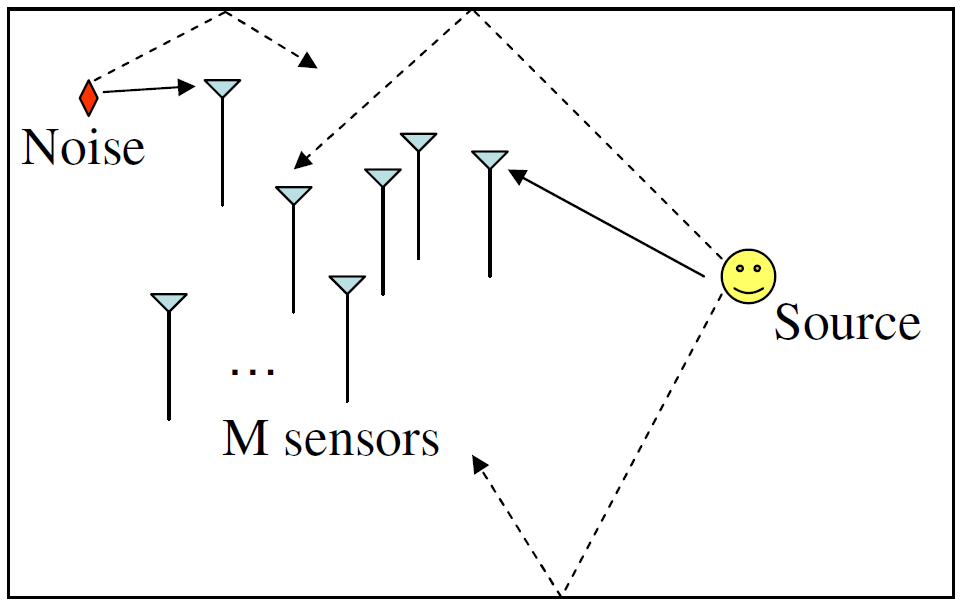
\includegraphics[scale=0.7]{observation_model.png}
	\caption[Room representation for the observational model \cite{ba2007}]{A source incident on an array of M sensors in the presence of noise and reverberations \cite{ba2007}}
	\label{fig:observation}
\end{figure}

In the Fourier domain the received signal described in equation \ref{eq:observationtime} for microphone $i$ can be written as:
\begin{equation}
\label{eq:observationfreq}
Y_{i}(\omega) = A_{i}(\omega)S(\omega)e^{-j\omega\tau_{i}} G_i(\omega,\theta,\phi) + V_{i}(\omega)
\end{equation}

\nomenclature{$Y(\omega)$}{Received audio signal by a microphone in the frequency domain}
\nomenclature{$A(\omega,\theta,\phi)$}{Attenuation coefficient in the frequency domain, as a function of the look direction}
\nomenclature{$S(\omega)$}{Source signal in the frequency domain}
\nomenclature{$G(\omega,\theta,\phi)$}{Directivity pattern of a microphone in the frequency domain}
\nomenclature{$V(\omega)$}{Undesired signal components in the frequency domain}


The attenuation factor $A_{i}(\omega)$ can depend on the frequency. $G_i(\omega,\theta,\phi)$ is the directivity pattern of the microphone in the Fourier domain, for nonuniform directivity microphones on the respective azimuth and elevation; $V_{i}(\omega)$ is the additive noise in the Fourier domain.

By choosing the values for $A_{i}(\omega,\theta,\phi)$ and $\tau_{i}$ one can maximize the gain (or steer the beam) in any direction spanned by the position vectors of the array. The desired signal can be recovered by multiplying the microphone signals by a complex weighing factor $\textbf{w}$:

\begin{equation}
\label{eq:bf_est}
\hat{S}(\omega) = \textbf{w}^{H}(\omega)\textbf{Y}(\omega)
\end{equation}

\nomenclature{$\hat{S}(\omega)$}{Estimated source signal}
\nomenclature{$\textbf{w}(\omega)$}{Vector of complex weighing factors}

where $\textbf{a}^{H}$ denotes the Hermitian transpose of the vector $\textbf{a}$. The estimated signal $\hat{S}(\omega)$ can finally be transferred back to the time domain to arrive at the beamformed audio signal. Sections \ref{sec:des_dsb} and \ref{sec:des_mvdr} go into how to calculate the weights $\textbf{w}(\omega)$.

\chapter{Related research}
\label{chap:related}
With the increase of smartphone usage it is no surprise that a lot of research has been done considering beamforming algorithms. Many different algorithms have been proposed to use to perform beamforming with \cite{vanveen1988, griffiths1982, krim1996}. In this chapter, related research relevant to this topic will be discussed.

First common methods and the state of the art in beamforming research for acoustic and speech enhancement will be discussed. Then the different measures to evaluate the performance of these algorithms are introduced and to conclude ways to implement localization on the smartphones and distributed computation of the beamforming algorithm will be looked into.

\section{Beamforming Algorithms}
\label{sec:rel_beamformers}

Microphone arrays are a common way to improve sound quality; the diversity in the received signals is exploited by setting different gains to each microphone, depending on the location of the source and on the auxiliary sources and noise. This is generally referred to as beamforming. There are different beamforming algorithms each with their own advantages and disadvantages. The delay-and-sum beamformer (DSB) is one of the earliest beamforming algorithms. It is a "fixed" beamformer, meaning that it only adapts to the locations of the microphones and the desired source. It delays and optionally weighs the microphone signals based on the distances and the speed of sound and the attenuation of the soundwave respectively before taking the average of the signals. The MVDR beamformer is one of the most widely used beamformers and can be used for both speech dereverberation and noise reduction \cite{naylor2010speech}.

\subsection{Delay-and-sum Beamformer}
The delay-and-sum beamformer (DSB) is an important approach to dereverberation and provides a reference to compare other methods with. The expected improvement in the Direct to Reverberant Ratio (DRR) of the DSB only depends on the distance between the source and  the array and the seperation of the microphones and does not depend on reverberation time, which is the time it takes for the reverberant energy to drop to 60 dB below the original level. When the microphones are seperated by a half wavelength, perfect dereverberation is achieved \cite{naylor2010speech}. For spatially white noise only, the DSB is the optimal beamformer \cite{brandstein2001}.

White noise in general is a random signal with a constant power spectral density. It has a constant bandwidth and does not depend on the frequency \cite{carter2013}. Spatially white noise means that the noise is uncorrelated amongst all sensors in the array \cite{krim1996}.

\subsection{Minimum variance distortionless response Beamformer}
The minimum variance distortionless response (MVDR) beamformer \cite{naylor2010speech} is one of the most widely used beamformers. This beamforming algorithm can suppress coherent noise sources well. However, in a spatially white noise field, the MVDR beamformer reduces to a DSB  \cite{naylor2010speech}. The MVDR is also excessively sensitive to source location and microphone gains \citep{ba2007}.

There are multiple proposed variations on the standard MVDR beamformer. The first variation on the steered beamformer based locators with an increased accuracy in reverberate rooms is proposed by Ba et al. \cite{ba2007}. This algorithm is specifically designed for directional microphones in a teleconference setting. The algorithm uses voice activity detection to differentiate between speech and noise in the sound at the input of the beamformer. The noise component of the input will be used to update the covariant matrix of the beamformer. The block diagram of this algorithm can be found in figure \ref{fig:emvdr}. 

In the research by Ba et al. \cite{ba2007} a comparison is made between an MVDR beamformer with and without gain compensation for the microphone directivity. However, only circular microphone arrays are considered in this paper. The proposed eMVDR, which stands for enhanced MVDR, algorithm with the directivities included, outperforms the traditional MVDR in all ten of the experimented scenarios.
\begin{figure}
	\centering  
	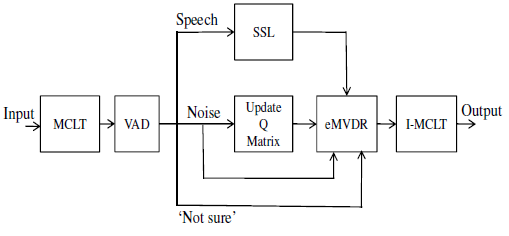
\includegraphics[scale=1]{Blockdiagram_emvdr.png}
	\caption{Block diagram of the eMVDR \cite{ba2007}} 
	\label{fig:emvdr}
\end{figure}
A different variation on the MVDR, which includes directivities in the beamformer, is proposed by Gaubitch et al. \cite{gaubitch2014}. This research also concludes that including the directivities in the beamformer significantly increases the performance of the beamformer. 



\subsection{Other beamforming algorithms}
Another beamforming algorithm, which is proposed by Martinez et al. \cite{martinez2015}, uses an eigenfilter structure to focus on regions instead of just an angle. The consequence of this variation is an increase in the robustness of the beamformer.

Another kind of beamformer is the generalized sidelobe canceller (GSC) \cite{griffiths1982}. One of the disadvantages of this beamformer is the robustness problem \cite{brandstein2001}. The beamformer suffers from target-signal cancellations due to errors in the steering vector. The generalized sidelobe canceller computes the weight factors in a different way than the MVDR beamformer resulting in a much lower complexity.

\section{Evaluation of the Beamforming techniques}
To investigate the performance of our algorithms, the results will be evaluated using different intelligibility measures \cite{taal2010,rix2001}.
The measures used to evaluate a beamformer are power related measures and intelligibility measures. The power related measure show a ratio between powers, for example the SNR shows the ratio of signal to noise. This can be used to determine if a beamforming algorithm suppresses the noise while keeping the signal power the same. Intelligibility measures determine the extend to which a signal is understandable for speech applications. In this thesis the beamforming algorithms are used to enhance speech, which is why the intelligibility measures are interesting to investigate.

Different power related measures exist which can be used to investigate the performance of a beamformer. A few of them are:

\begin{itemize}
\item Global SNR[dB]
\item Segmental SNR [dB]
\item White noise gain
\item Array-gain
\end{itemize}

The global and segmental SNR are calculated by determining the ratio between the power of the signal and the power of the noise. The global SNR uses the complete signal to determine this ratio. The segmental SNR calculates the average SNR of only those frames of the sound signal which exhibit an SNR larger than $0 dB$ \cite{brandstein2001}. The segmental SNR measures the amplitude distortion of the sound signal and will therefore be well correlated with perceived distortions. 

The shows the ability of a beamformer to suppress spatially uncorrelated noise \cite{brandstein2001}. White noise gain is defined as the output power due to unit variance white noise in the sensor \cite{vanveen1988}.  The white noise gain is represented by $\textbf{w}^H\textbf{w}$. If the white noise gain is high, the beamformer output will have a poor SNR due to white noise contributions. 

The array-gain shows the improvement of the signal-to-noise ratio between one of the microphones and enhanced output of the array and can be calculated as follows:

\begin{equation}
G_{A} = \frac{\text{SNR}_\text{{array}}}{\text{SNR}_\text{microphone}}
\end{equation}

\nomenclature{$G_\text{A}$}{Array-gain}
\nomenclature{$SNR$}{Signal-to-noise ratio [dB]}

An intelligibility measure that shows a good correlation with speech intelligibility is the Short-Time Objective Intelligibility measure (STOI) \cite{taal2010, taal2011}. STOI is based on the correlation between short-time segments of the clean and processed signal. The short-time segments used were approximately $400 ms$. This algorithms was specifically designed for a sample-rate of $10000 Hz$ to cover the relevant frequency range for speech. The STOI is expressed in the range $0$ to $1$ where a higher value means that the signal is more intelligible.

\nomenclature{STOI}{Short-Time Objective Intelligibility measure}

Another widely used intelligibility measure is Perceptual Evaluation of Speech Quality (PESQ). PESQ predicts the perceived quality that would be given to the processed signal by subjective listening tests. This measure shows a high correlation with the subjective Mean Opinion Scores (MOS) \cite{rix2001, itu2010}.

The mean opinion score is a test that results in an indication of the quality of a phone call on a scale from $1$ to $5$, where $1$ stands for bad and $5$ stands for excellent. There are guidelines, given by ITU-T recommendation $P.800$ \cite{ituquality1998}, for the environment of the speaker that should be followed when conducting such a test.

It is expected that an improvement in SNR results in an improvement in MOS \cite{itumos1996}. This means that the PESQ should also improve since MOS and PESQ show a high correlation. 

\nomenclature{MOS}{Mean opinion scores}
\nomenclature{PESQ}{Perceptual evaluation of speech}
\chapter{Describing the design process}
\label{chap:design}
% Design: formules, inputs, outputs etc

%algemeen beamforming							(Niels)
%Beamformers provide an effective and versatile means of spatial filtering \cite{vanveen1988}. 
Beamformers are useful when distinguishing desired signals from noise and interference based on their locations \cite{himawan2011}. There are different beamforming algorithms with their own advantages and disadvantages. 

In this research, the delay-and-sum beamforming algorithm \cite{elko1996} and the MVDR algorithm \cite{habetsspeech2010} will be discussed. The DSB will be considered since this is a good baseline method to compare the other beamformer with. The MVDR has been chosen since the generalized sidelobe cancellar beamformer suffers from steering vector errors and the MVDR suppresses coherent noise well.


%The original MVDR is excessively sensitive to source location and microphone gains \citep{ba2007}. Microphone arrays are a common way to improve sound quality; the diversity in the received signals is exploited by setting different gains to each microphone, depending on the location of the source and on the auxiliary sources and noise. This is generally referred to as beamforming. There are different beamforming algorithms each with their own advantages and disadvantages. The delay-and-sum beamformer (DSB) is one of the earliest beamforming algorithms. It is a "fixed" beamformer, meaning that it only adapts to the locations of the microphones and the desired source. It delays and optionally weighs the microphone signals based on the distances and the speed of sound and the attenuation of the soundwave respectively bofore taking the average of the signals. The MVDR beamformer is one of the most widely used beamformers and can be used for both speech dereverberation and noise reduction.

%and a broadband region-based near-field beamforming algorithm \cite{martinez2015} that we refer to here as the ``Delft'' algorithm.

%In the scenario outlined in section {\ref{chap:introduction}} the dimensions of the microphone array are large with respect to the distance between the array and the source. Therefore we can assume that the sources of interest are mostly in the near-field region \cite{gaubitch2014}. In addition, the positioning of the microphones is arbitrary, but known. As such, the main focus for our implementation will be near-field beamforming with ad-hoc microphone arrays. In particular, we will research the benefits of compensating for the directivities of the microphones in the smartphones, as \cite{gaubitch2014} shows this having a positive effect on beamformer performance. To estimate the performance of our algorithms, the results will be evaluated using different intelligibility measures \cite{taal2010,rix2001}.

\section{Simulation}
\label{sec:des_simulation}

In this research, a simulation is used to simulate the effect of a reverberant room on the acoustic signals received at multiple microphones. This algorithm has been implemented in \matlab to simulate recording multiple audio sources in a room with multiple microphones. The simulation will be used to compare to the experimental results. The acoustic impulse response of a room characterizes the acoustics of that room. The convolution between the sound coming from the source and the impulse response results in the sound recorded by the microphones. The simulated microphones are omnidirectional, which means that the directivities of the microphones are not included in this simulation.

The parameters that can be set for this simulation are:

\begin{itemize}
\item Locations of the audio sources and the microphones. 
\item Size of the room.
\item Reflection coefficients.
\item SNR at which Gaussian white noise will be added.
\item Amount of random errors added to the microphone positions.
\item Reverberations on or off.
\end{itemize} 

Local stored audio files are expected as source files. The audio files will be trimmed down or zero padded to match the simulation time. Then the implemented algorithm calculates the impulse response of a room. The locations of the sources and the locations of the microphones and the size of the room will be used to calculate the impulse response between each source and each microphone. The impulse response is calculated using the image method \cite{allen1979}. This method mirrors the walls of a room and puts the sources in imaginary rooms next to the room in which the source and receiver are placed. This concept is illustrated in figure \ref{fig:image_method}. The standard image method has been modified to simulate received echo arrival time to estimate the intermicrophone phase \cite{peterson1986}.

\begin{figure} [h]
    \centering
       \includegraphics[page=2, scale = 1, clip=true, trim=10.5cm 23.3cm 4.5cm 1.5cm]{image_method.pdf} % l b r t
    \caption[Image method for simulating a rooms \cite{allen1979}]{Image method, "x" stands for an audio source and an "o" stands for a microphone. \cite{allen1979}}
    \label{fig:image_method}
\end{figure}

After calculating the impulse response of the room it is possible to determine the signal recorded by each microphone. The convolution of the source signals with the impulse responses result in an output signal for each microphone.

This is done by calculating the convolution between the impulse response of the room and the associated audio source. After this is done for each audio source and each microphone, white noise is added to make the simulation more realistic.

Having implemented this algorithm, the choice can be made to either record audio and apply the beamforming algorithm to that or use the simulation to create the input for the beamforming algorithm. The simulation calculates the acoustic impulse of the room which will be used to generate the sound recorded by the microphones. One of the impulse responses for a simulation without reverberations and one impulse response for a simulation with reverberations is plotted and can be found in figure \ref{fig:imp} and \ref{fig:impRev}.


\begin{figure}
	\centering  
	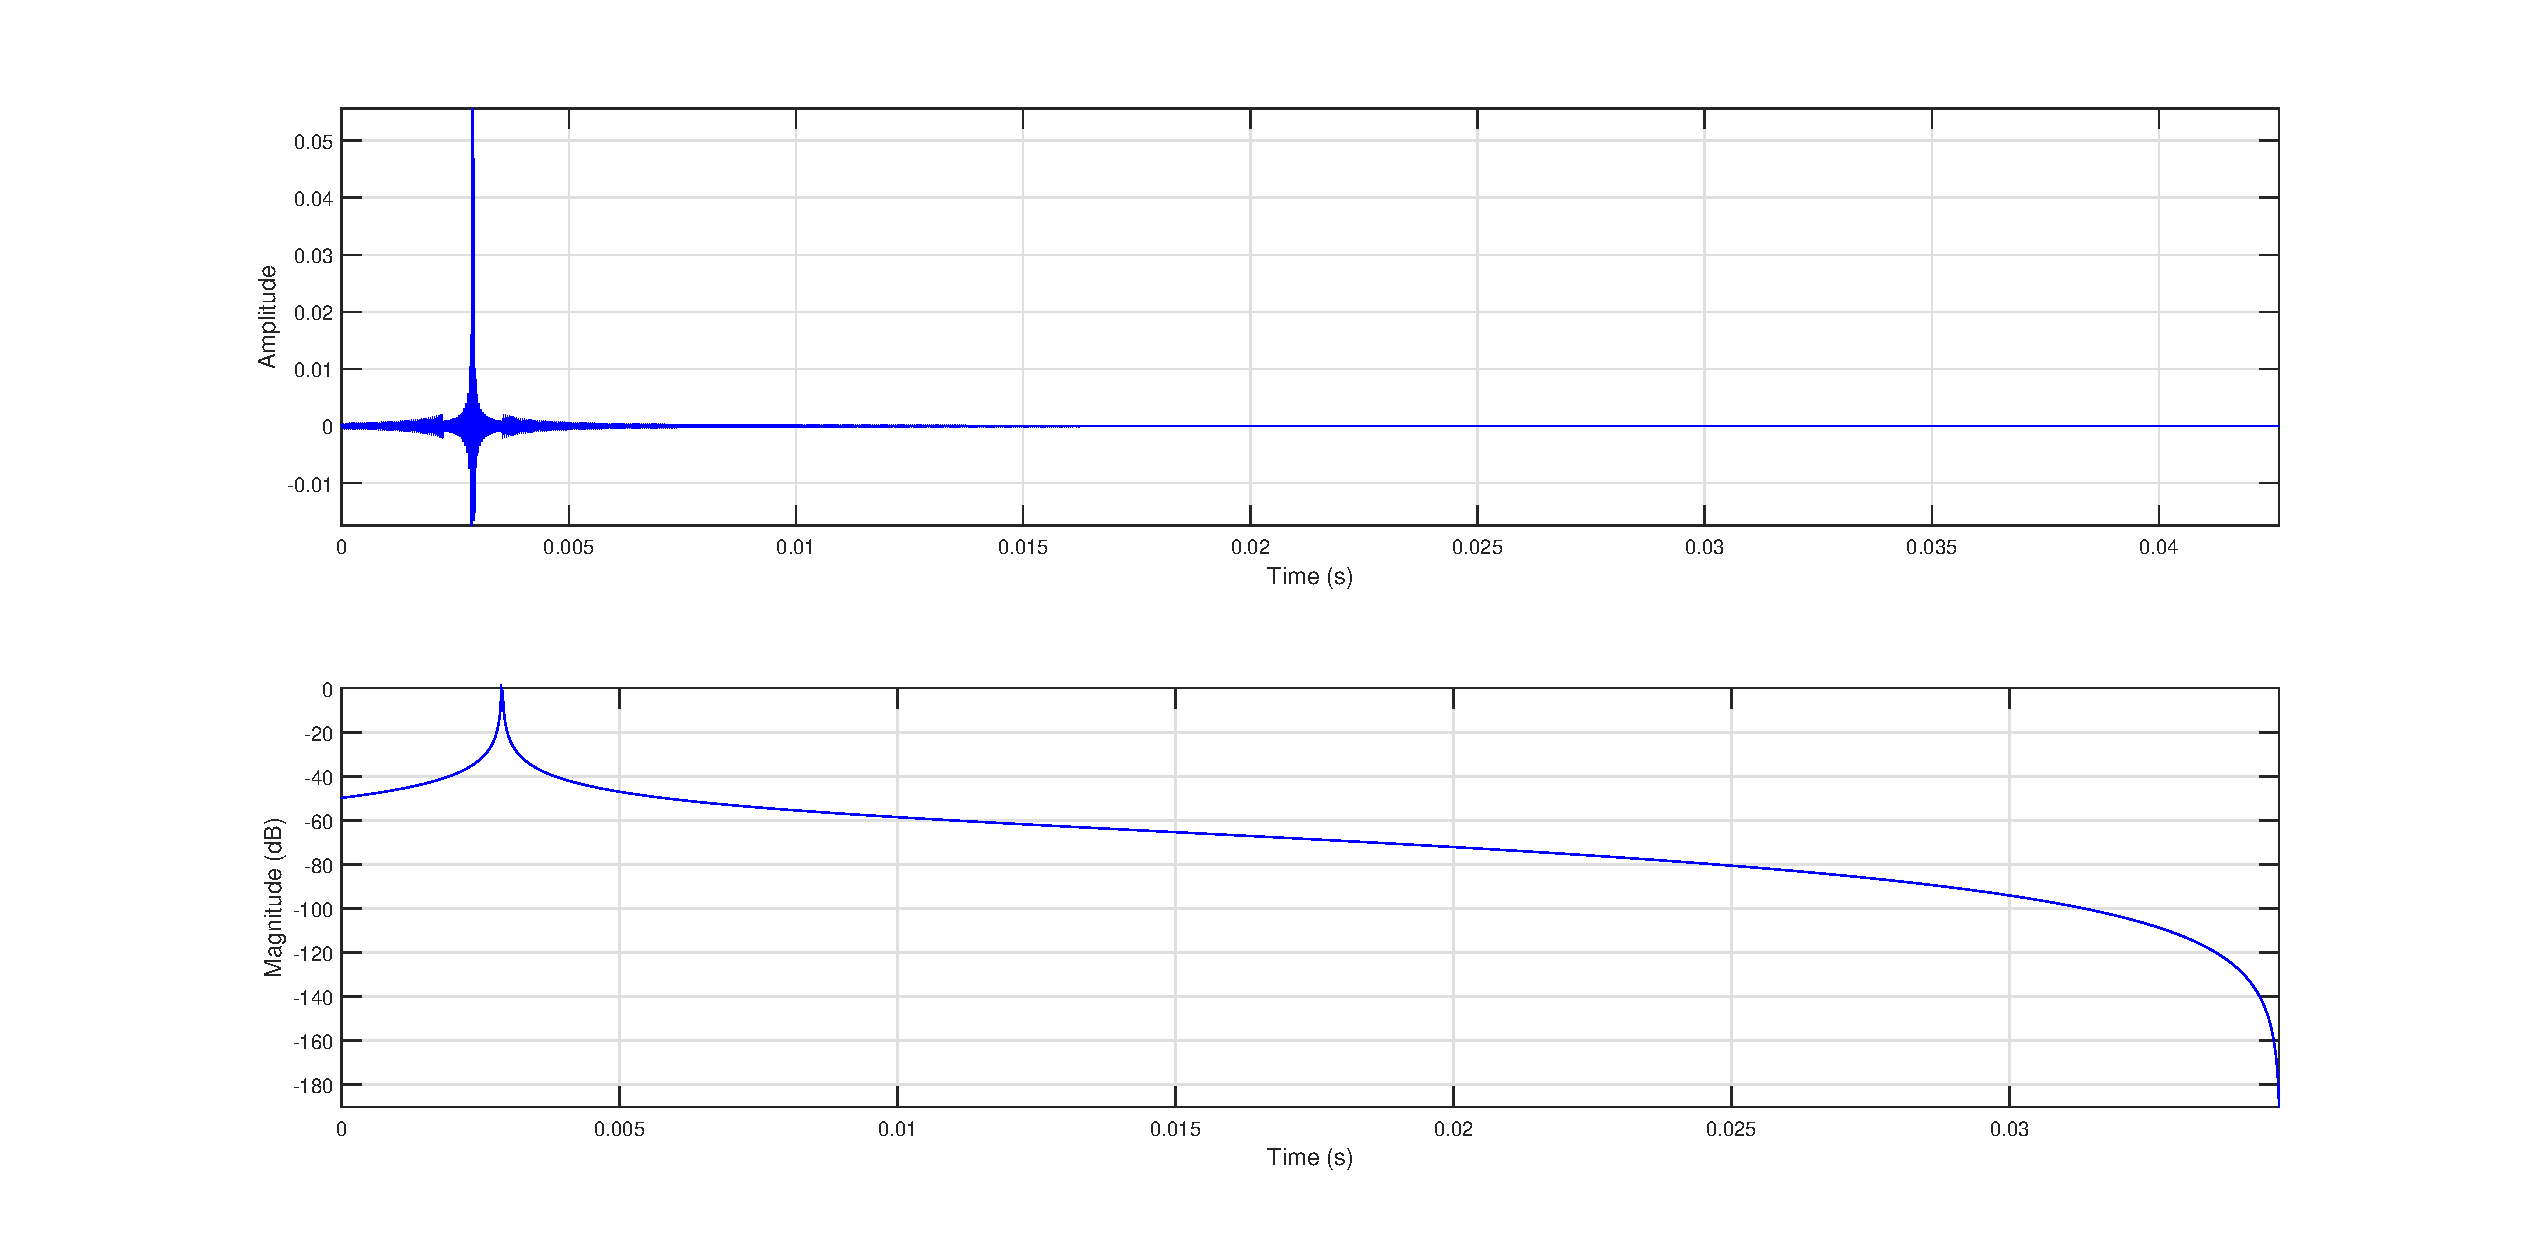
\includegraphics[width = 0.8\columnwidth, clip=true, trim= 0 1.1cm 0 0]{Screenshots_simulatie/Impulse_response/Simulatie_3}
	\caption[Simulated Impulse response without reverberations]{Simulated impulse response without reverberations in time-domain} 
	\label{fig:imp}
\end{figure}

\begin{figure} [h!]
	\centering  
	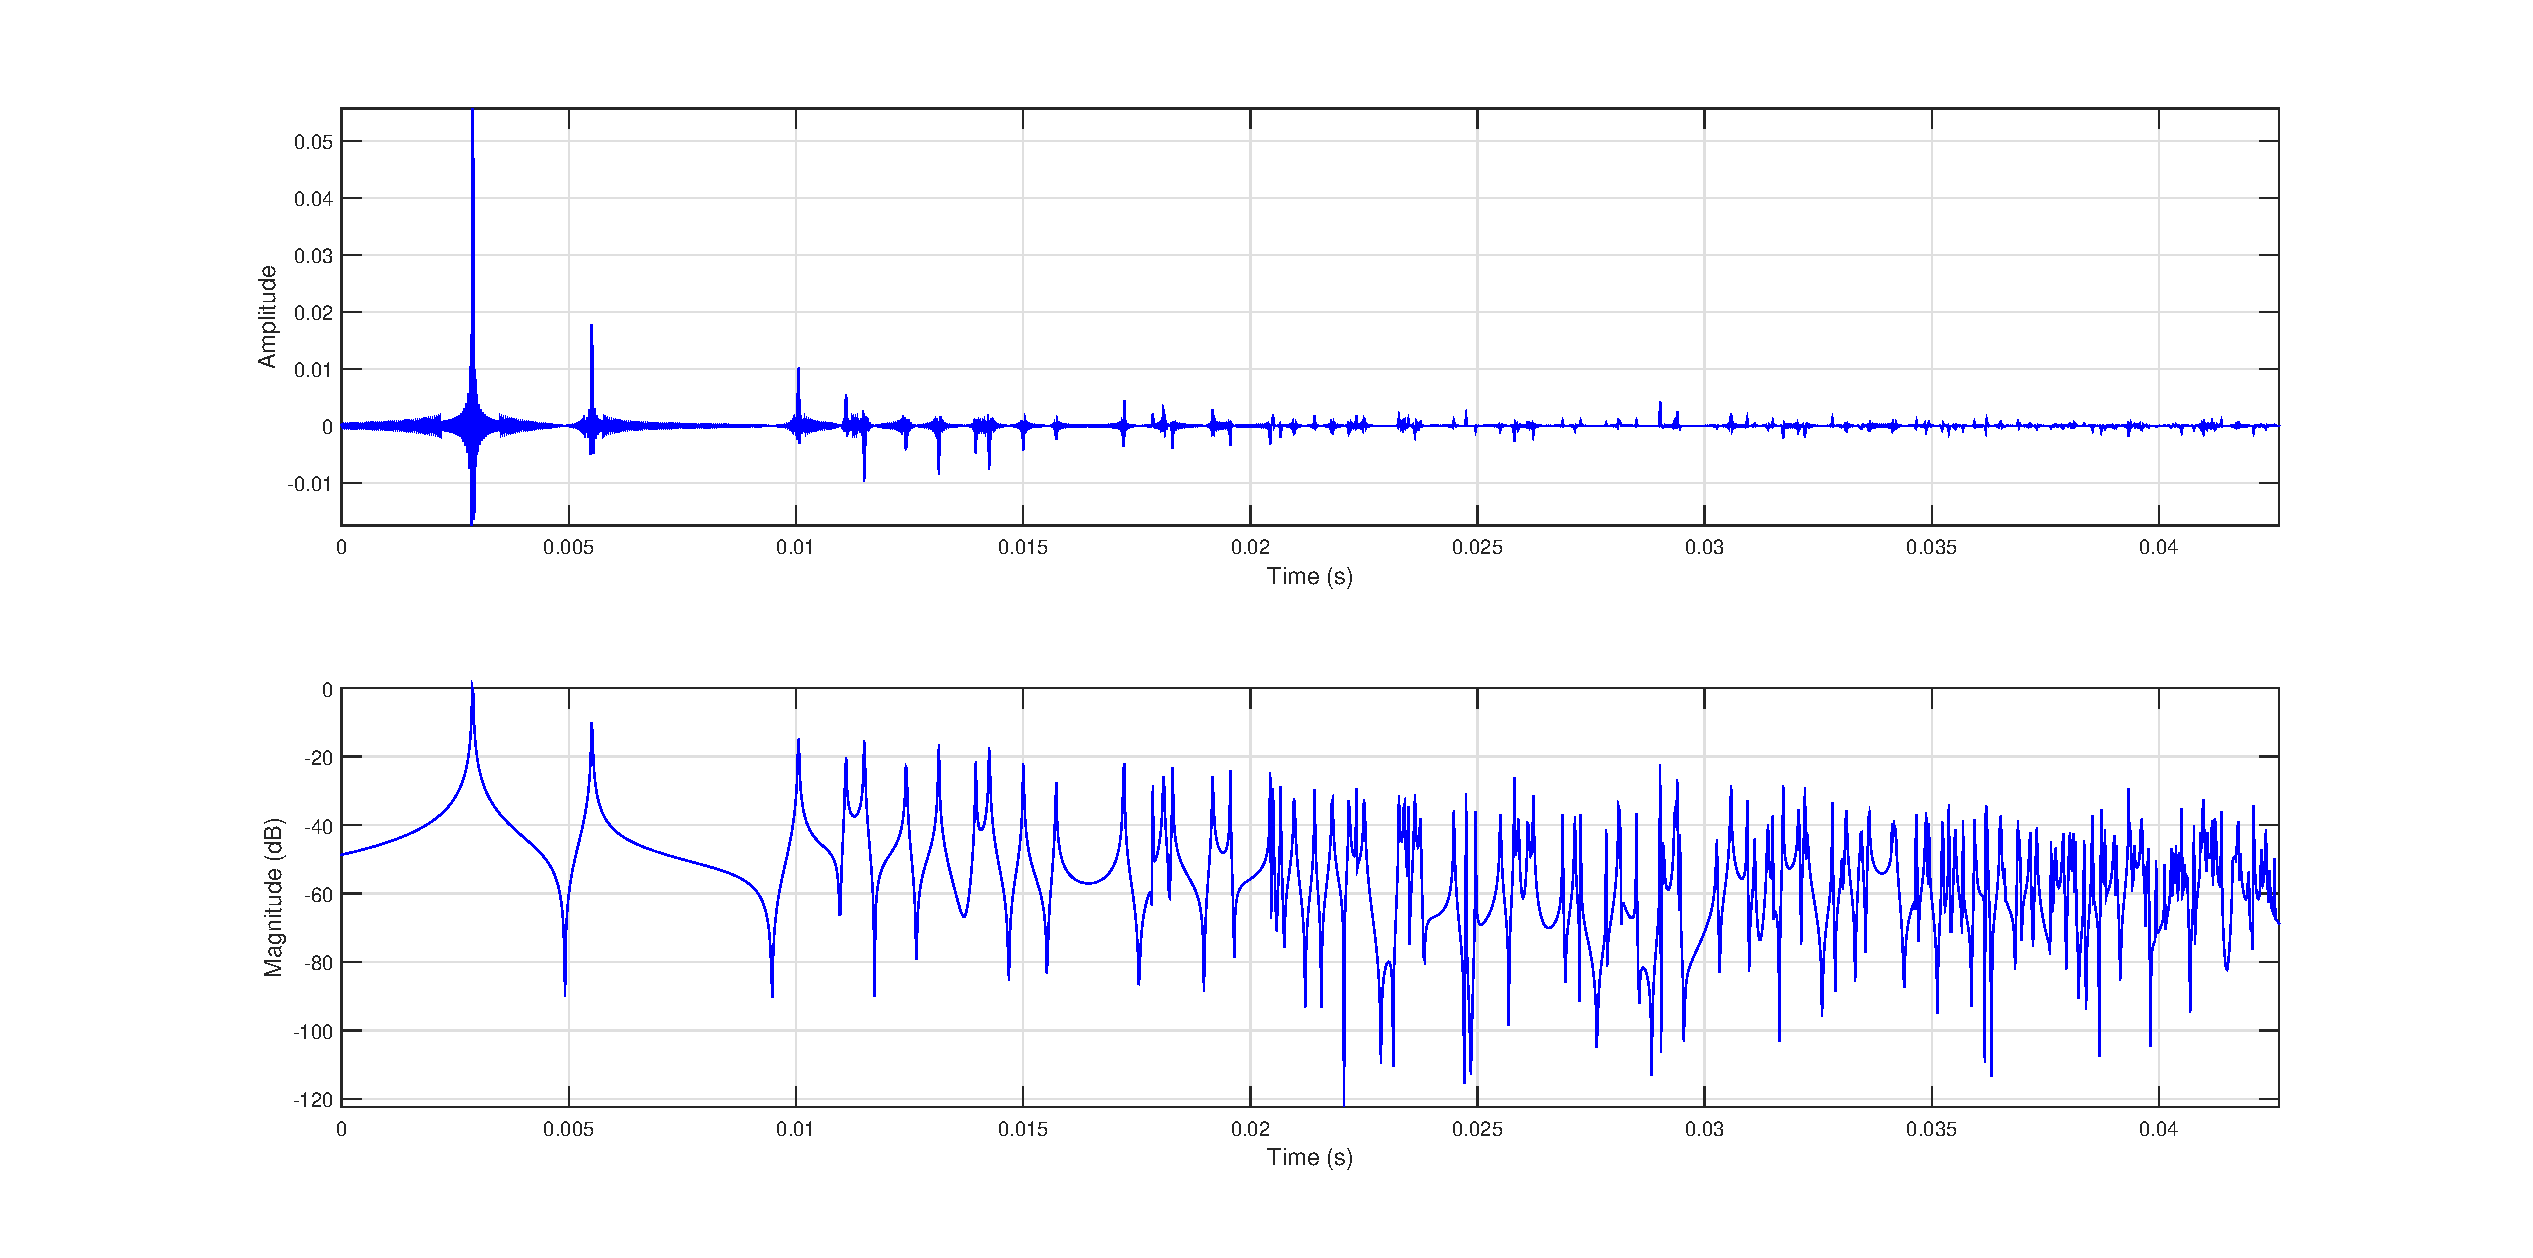
\includegraphics[width = 0.8\columnwidth, clip=true, trim= 0 1cm 0 0]{Screenshots_simulatie/Impulse_response/Simulatie_4}
	\caption[Simulated Impulse response with reverberations]{Simulated impulse response with reverberations in time-domain} 
	\label{fig:impRev}
\end{figure}

\section{Beamforming}
\label{sec:des_beamforming}
The technique called beamforming combines sensor array signals in some optimal manner such that the output approximates the desired source and suppresses the undesired noise/interferers. By choosing sensible weights a beamformer can perform spatial filtering with the goal of maximizing the intelligibility of the received signal.

The goal of beamforming is to estimate the desired signal $\hat{S}$ from equation \ref{eq:bf_est} as a linear combination of the data collected at the array. In other words, we would like to determine an $M \times 1$ vector weights $w(\omega)$ such that $\textbf{w}^{H}(\omega)\textbf{Y}(\omega)$ is a good estimate of $S(\omega)$.

The delay-and-sum beamformer (DSB) is one of the earliest beamforming algorithms. It is a "fixed" beamformer, meaning that it only adapts to the locations of the microphones and the desired source. The MVDR beamformer is one of the most widely used beamformers and can be used for both speech dereverberation and noise reduction.

%\nomenclature{$w$}{Weight in the frequency domain}

\subsection{Delay-and-sum Beamformer}
\label{sec:des_dsb}
%Erik
The delay-and-sum beamformer (DSB) first delays and weighs the microphone signals and then sums or averages the results for all the microphones. For the simple DSB the complex weights $\textbf{w}$ usually consists of only the delays. In near-field (Section \ref{sec:problem_near-field} applications the DSB may also perform inverse distance weighing in addition to delaying the signal to correct for attenuation losses. In the time domain the output $\overline{x}[n]$ can be written as \cite{naylor2010speech}:

\begin{equation}
\overline{x}[n] = \sum_{i=1}^{M} w_{i}x_{i}[n-\tau_{i}]
\end{equation}

\nomenclature{$\overline{x}(n)$}{Average estimated clean speech signal in the time domain}

%Delay-and-sum
If we take the discrete time Fourier transform and move the delay into the weight we get for the weights $\textbf{w} = [w_1,w_2,\dots,w_i,\dots,w_M]$: 

\begin{equation}
w_i(\omega) = \frac{1}{M} e^{-j\omega\tau_i}
\end{equation}
or with inverse distance weighing:
\begin{equation}
w_i(\omega) = \frac{1}{4\pi r_{i} M} e^{-j\omega\tau_i}
\end{equation}

with $M$ the number of microphones, $i \in \{1,2,\dots,M\}$, $w_{i}$ the weight applied to the $i^{th}$ microphone and $\tau_{i}$ the propagation delay in samples. This weight can be used to estimate the source signal described in equation \ref{eq:bf_est}. \newline
The best asset of the DSB is that the direct path components of the microphone signals will be coherent and therefore added constructively. The incoherent components, due to reverberation and noise, will be attenuated.

\subsection{Minimum variance distortionless response Beamformer}
\label{sec:des_mvdr}
%Erik
A general description of MVDR beamformers in room acoustics and the trade-off between speech dereverberation and noise reduction is described by Cohen et al.\cite{habetsspeech2010} and Habets et al. \cite{habetsroom2010}. The MVDR beamformer is derived by minimizing the energy of the observed signal, subject to the constraint that the signal in the desired look position remains undistorted \cite{vanveen1988}. It minimizes the variance of the noise component of $\textbf{w}^{H}\textbf{Y}$ from equation \ref{eq:bf_est}, subject to a constraint of gain 1 in the look direction \cite{ba2007}. The corresponding weight vector $\textbf{w}$ is the solution to the following optimization problem:

\begin{equation}
\hat{\textbf{w}} = \argmin_\textbf{w} \textbf{w}^H \Phi_\textbf{Y} \textbf{w} \quad\textrm{s.t.}\quad\textbf{w}^H\textbf{d} = 1
\end{equation}

\nomenclature{$\hat{\textbf{w}}$}{Vector of estimated complex weights}
\nomenclature{$\Phi$}{Covariance matrix of the microhone signals}

where $\Phi_\textbf{Y}$ is the covariance matrix of the observed signal\footnote{This is actually true for Minimum Power Distortionless Response (MPDR), for traditional MVDR the covariance matrix of the combined noise signals sould be used, e.g. the covariance matrix of the reflected paths and auxilary sources \cite{gannot2010}.}. $\Phi_\textbf{Y}$ is given by $\Phi_\textbf{Y} = E[\textbf{YY}^H]$, where $E[\bullet]$ denotes the expected value function. This optimization problem has an elegant closed-form solution published by Cox et al.\cite{cox1987}:

\begin{equation}
\label{eq:cox}
\hat{\textbf{w}} = \frac{\Phi_{\textbf{Y}}^{-1}\textbf{d}}{\textbf{d}^{H}\Phi_{\textbf{Y}}^{-1}\textbf{d}}
\end{equation}

The denominator of this equation contains a normalization factor which enforces the gain constraint in the look direction. The numerator contains the minimized energy information for MPDR, or minimized noise information for traditional MVDR, for the respective microphones.

\subsection{MVDR with Directivity}
\label{sec:des_mvdr_dir}
To illustrate how to include the microphone directivities in the algorithm a similar approach to Gaubitch et al. \cite{gaubitch2014} will be followed, which is outlined in this section. The theory of how to include directive (non-omnidirectional) microphones into the MVDR algorithm was briefly covered in section \ref{sec:observation}. The difference is not in the algorithm, but in the used impuls response. \newline
For omnidirectional microphones the signal received at each microphone ($Y_{i}$) consists of the following components:

\begin{equation}
Y_{i}(\omega) = S(\omega)H_{i}(\omega) + V_{i}(\omega)
\end{equation}

When the microphones are directive the signal is convolved with the microphone directivity $G(\omega, \theta, \phi)$. We end up with:

\begin{equation}
Y_{i}(\omega) = S(\omega)H_{i}(\omega)G_{i}(\omega, \theta, \phi) + V_{i}(\omega)
\end{equation}

The estimated source signal is again calculated by:
\begin{equation}
\hat{S}(\omega) = \textbf{w}^{H}(\omega)\textbf{Y}(\omega)
\end{equation}

with the weights estimate from equation \ref{eq:cox}.

\section{Assessing Beamforming Quality}
\label{sec:des_evaluation}
%Niels
Six measures are used to evaluate the performance of the beamformer. Speech intelligibility is evaluated by the objective intelligibility measures PESQ and STOI. The other measures that are used are the global and segmental SNR, the white noise gain and the array gain.

The PESQ and STOI algorithms both compare the original and processed signal. The chosen implementation of the PESQ is the ITU-T recommendation P.862 in 2002 \cite{itu2010}. A general overview of the PESQ, given by the ITU-T Recommendation P.862, is illustrated in figure \ref{fig:PESQ_overview}. First, the delays between the original and processed signal are calculated to align the signals in time. Based on the delays, PESQ compares the signals using a perceptual model. This perceptual model is done by transforming the signals to an representation that is analogous to the psychophysical representation of audio signals in the human auditory system. The final step of the PESQ algorithm is using a cognitive model to compute two error parameters, one without and one with an asymmetry factor \cite{rix2001}.  These parameters are combined to give an objective listening quality MOS. The output of the PESQ is a number in the range of $-0.5$ to $4.5$, where $-0.5$ is the lowest quality and $4.5$ is the highest quality.

\begin{figure}
    \centering
       
\includegraphics[page=11, scale = 1, clip=true, trim=3.5cm 5.3cm 3.5cm 15.65cm]{PESQ.pdf} % l b r t
    \caption[General overview of the PESQ algorithm \cite{itu2010}]{Overview of the PESQ algorithm \cite{itu2010}}
    \label{fig:PESQ_overview}
\end{figure}

The other intelligibility measure used to determine the performance of the beamformer was STOI. The used algorithm was proposed and implemented by taal et al. \cite{taal2010,taal2011}.

The SNR is calculated by dividing the power of the signal by the power of the noise by the following equation:\cite{kondo2012}

\begin{equation}
\text{SNR} = 10log_{10} \frac{\sum_{n=1}^{N} x^2(n)}{\sum_{n=1}^{N} \{x(n) - \hat{x}(n)\}}
\end{equation}

Where x(n) is the clean speech signal, $\hat{x}(n)$ is the distorted speech and N is the number of samples.

\nomenclature{$x(n)$}{Clean speech signal in the time domain}
\nomenclature{$\hat{x}(n)$}{Distorted speech signal in the time domain}
\nomenclature{$N$}{Number of samples}

The classical SNR is not well related to to the speech quality and therefore the segmental SNR ($SNR_{seg}$) will also be calculated. $SNR_{seg}$ calculates the SNR in short frames and then takes the average of the frames. 

\begin{equation}
SNR_{seg} = \frac{10}{K} \sum_{k=0}^{K-1} log_{10} \frac{\sum_{n=L_{f}k}^{L_{f}k+L_{f}-1} x^2(n)}{\sum_{n=L_{f}k}^{L_{f}k+L_{f}-1} \{x(n)-\hat{x}(n)\}^2}
\end{equation}
Were $L_{f}$ is the frame length and $K$ the number of frames in the signal. By determining the energy in each frame it is possible to limit This calculation to the frames in which speech is active. The audio frames without speech will be discarded.

\nomenclature{$\text{SNR}_\text{seg}$}{Segmental signal-to-noise ratio [dB]}
\nomenclature{$L_{f}$}{Frame length of the segmental signal-to-noise ratio [s]}

\section{Realtime Beamforming Toolbox}
\label{sec:des_gui}
To make it easier to repeat the beamforming experiments a \matlab toolbox has been developed. The approach of this toolbox is based on the Model-view-controller-model (MVC). Beamforming scripts (of which there are many available on the internet) can be coded into a standard processing unit to use them in real time. Changes to individual algorithms may have to be made to make them run in realtime and the input variables may have to be relabeled. \newline
In this section the implementation of the system is described. Figure \ref{fig:UI_schematic} shows a flowchart of the system. The green blocks (on the left side) are possible inputs. The orange blocks show inputs that have to be set from the UI. The rightmost blocks are the processing algorithms.

\begin{figure}
    \centering
       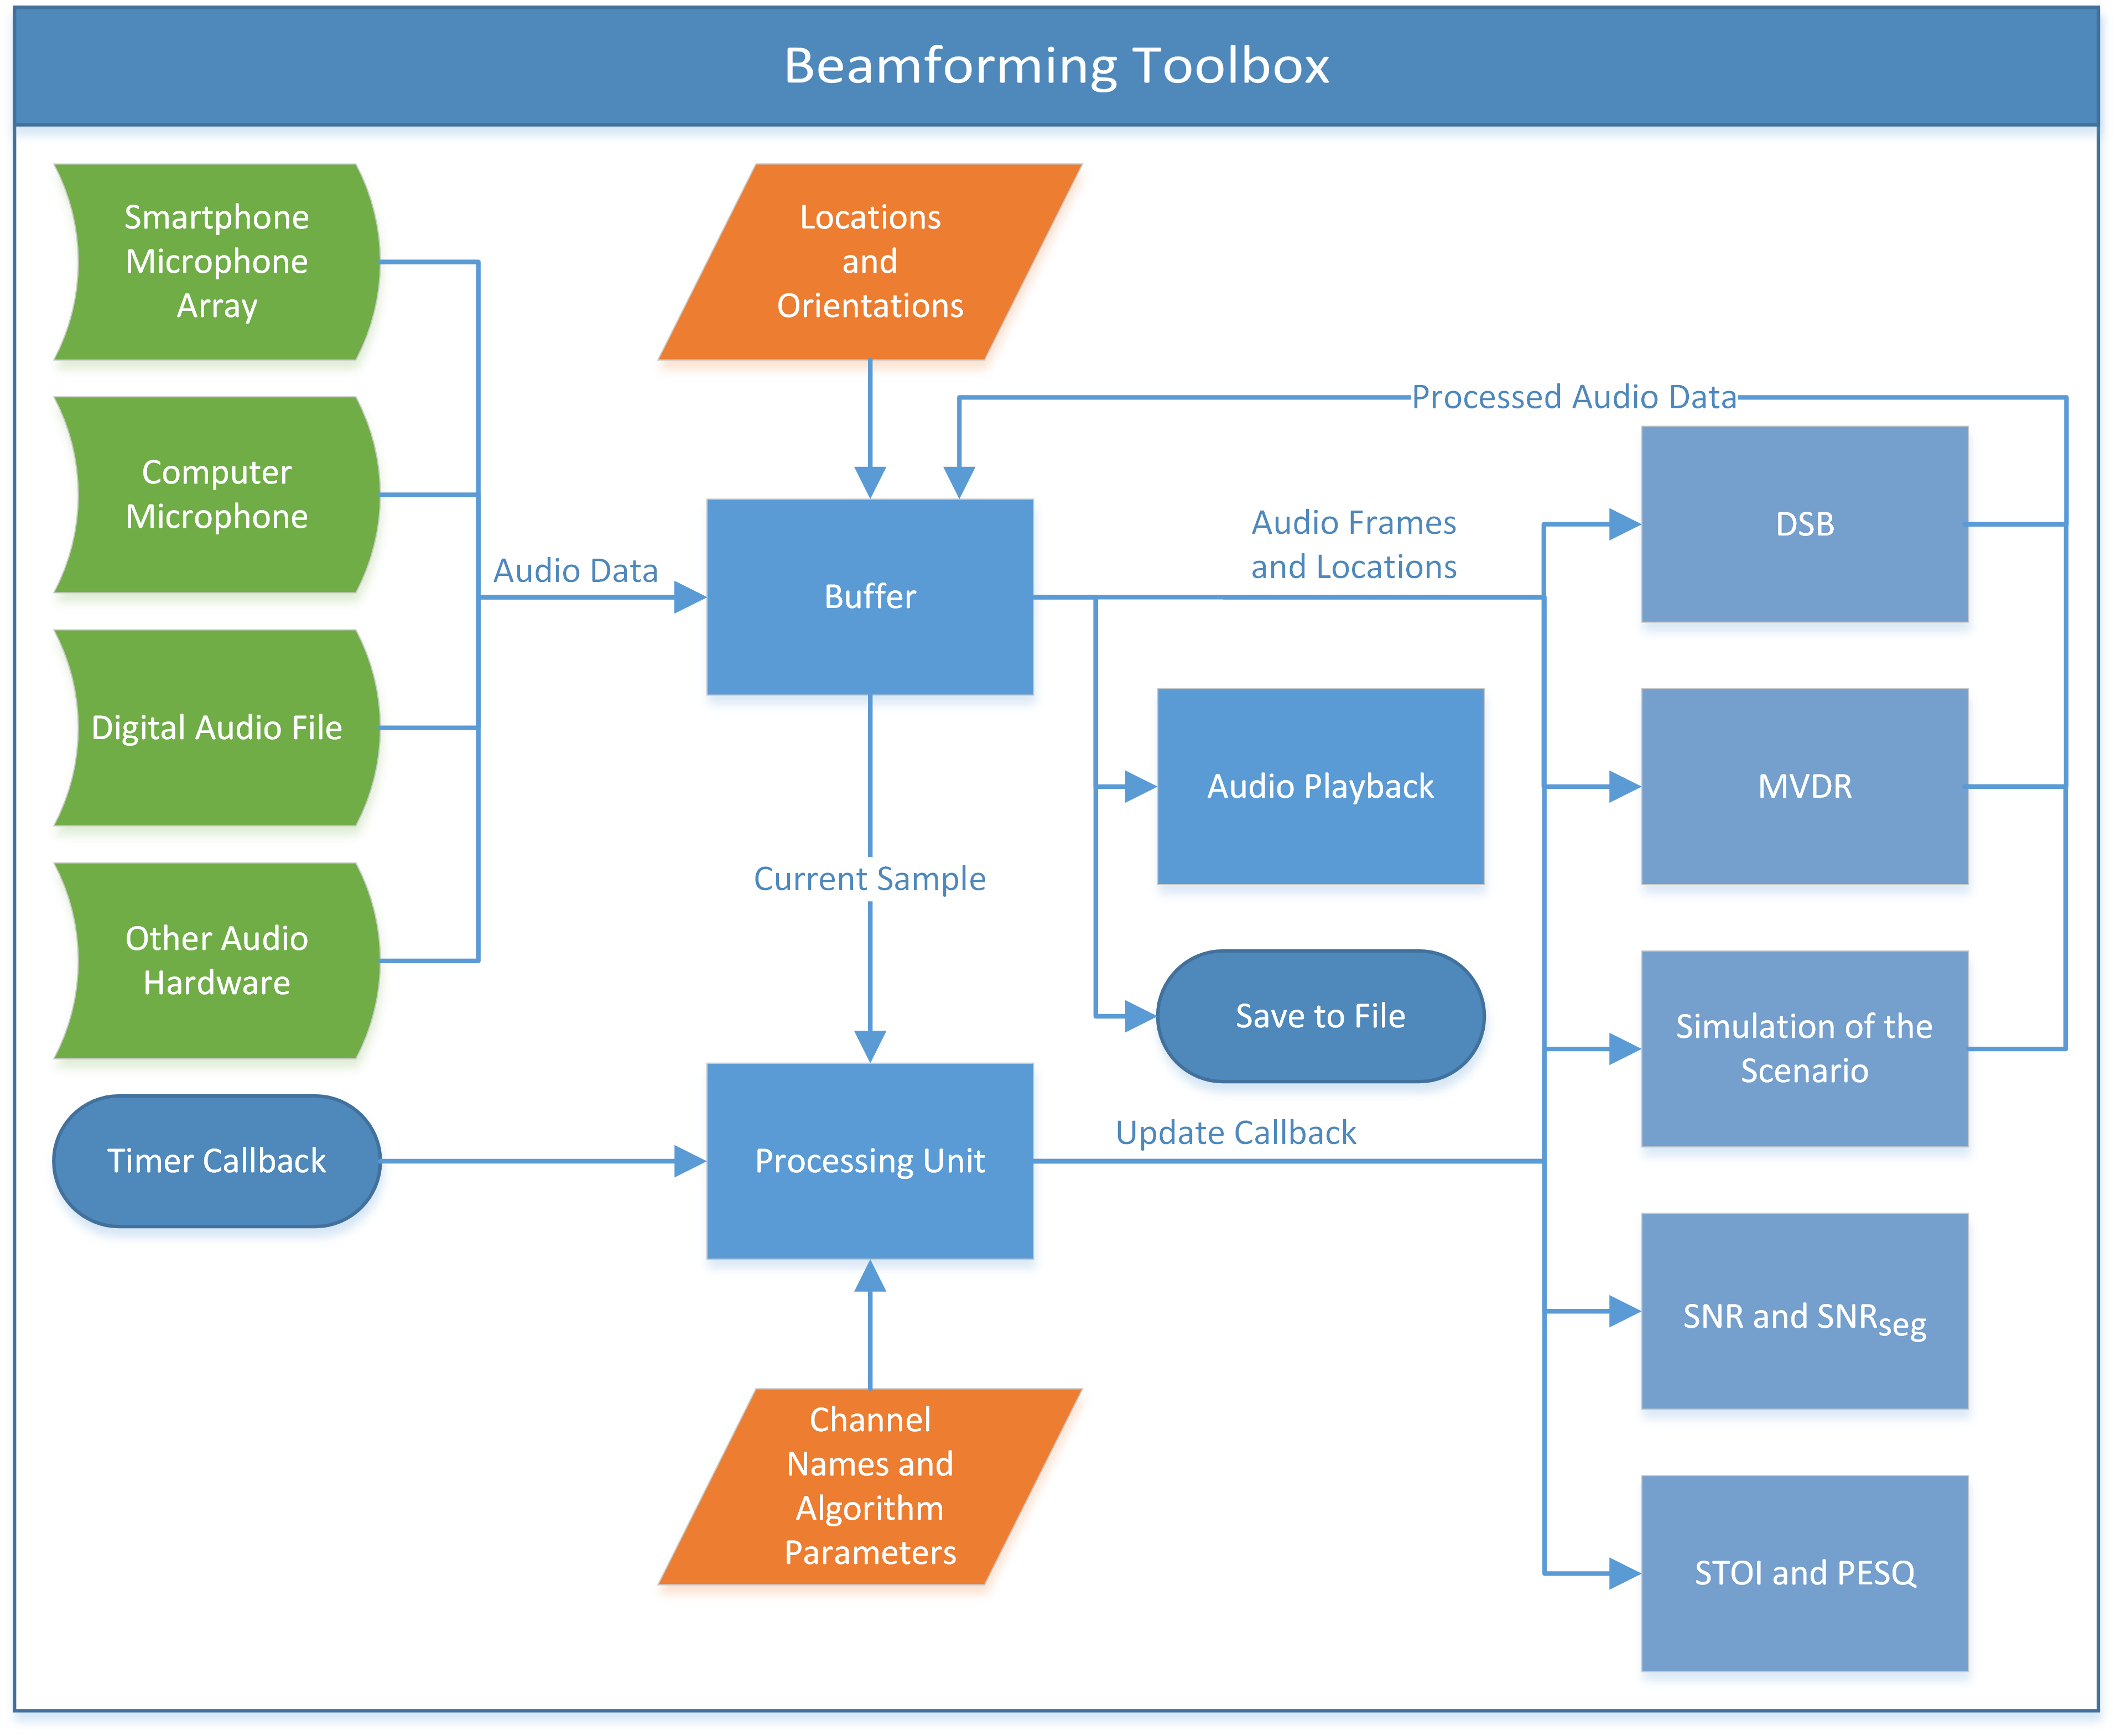
\includegraphics[scale = 0.6, clip = true]{images/beamforming_UI_schemetic.png} % l b r t
    \caption[Beamforming Toolbox flowchart]{Beamforming Toolbox flowchart.}
    \label{fig:UI_schematic}
\end{figure}

%\begin{figure} [b]
%    \centering
%       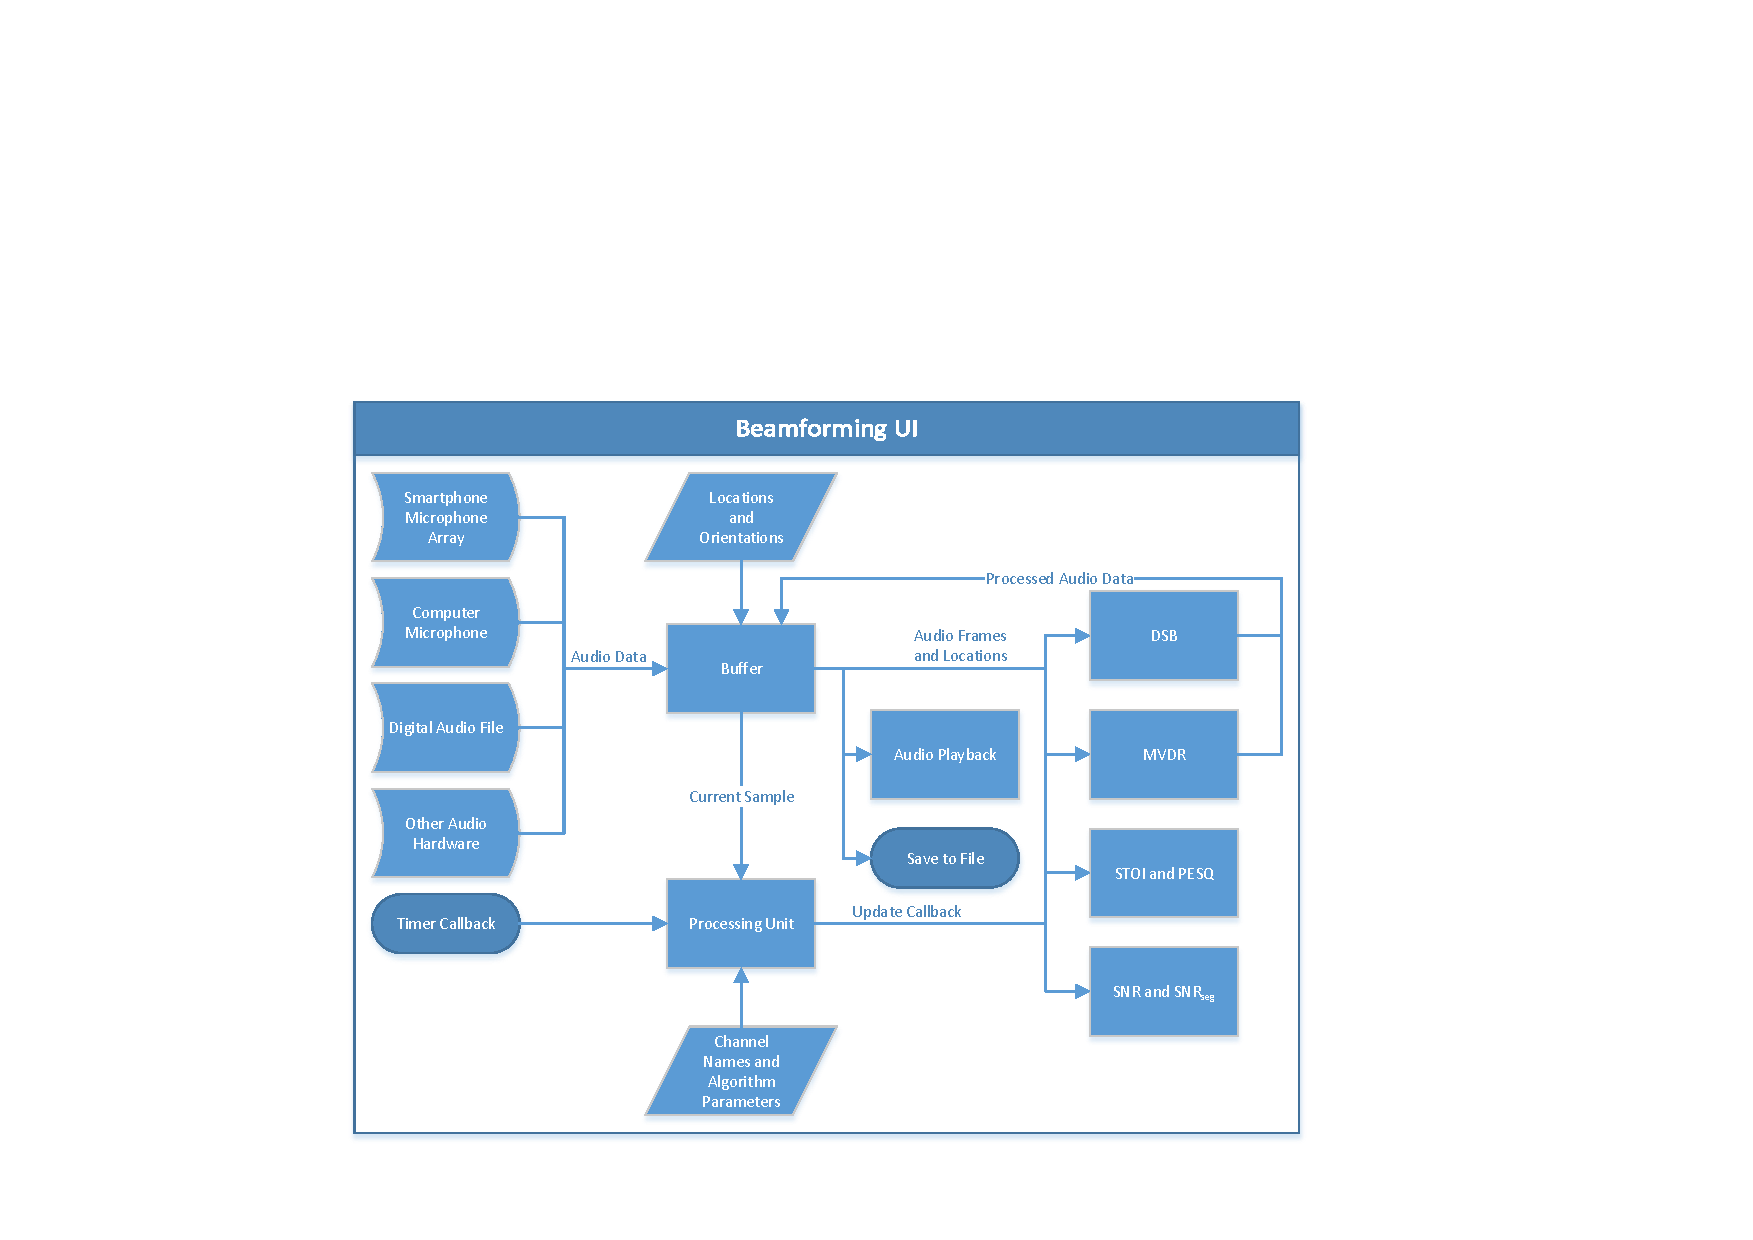
\includegraphics[scale = 1, clip = true, trim=10.5cm 23.3cm 4.5cm 1.5cm]{images/beamforming UI schemetic.pdf} % l b r t
%    \caption[Beamforming UI flowchart]{Beamforming UI flowchart.}
%    \label{fig:UI_schematic}
%\end{figure}

\subsection{Data Acquisition}
\label{sec:des_aqc}
Data inputs can be audio files, computer audio input channels, smartphones that run the Android app or multiple microphone locations can be simulated using different simulation options. Data from files can be loaded at once. The smartphones and computer microphones stream the data in small frames and call an update function when there is new data available. All inputs can be sampled at or resampled to other sample rates, but standard $48000 Hz$ is used. The data is usually sampled with a resolution of $16$ bits per sample, but as many steps in the computation require the data to be in double precision the data is stored in memory in double precision.


%Design process of Graphical user interface
%Erik

\subsection{Buffer}
\label{sec:des_buffer}
A fast data buffer has been implemented that serves as the core of the toolbox. All algorithms access the data so there need not be multiple copies of large data variables in memory. All of the used algorithms process the data in frames and write the processed data back to the buffer. This, in combination with proper memory allocation makes the toolbox run fast on large data sets as well as on smaller ones, as long as there is enough memory available. The buffer was tested with at most an hour of streaming audio from three smartphones, which resulted in about $3 GB$ of memory use. \newline
The properties of the data that are stored in the buffer are:
\begin{itemize}
\item Sample rate, $48000 Hz$
\item Bits per Sample, $16$
\item Number of Channels
\item Channel Name, reserved names are: $^*Mic, ^*Source, ^*Noise, ^*Beamformer$
\item Locations, $[x,y,z,az,el,up]$
\item Current Sample, stores the index of the last sample in the buffer for each channel
\item Total Samples
\item Audio Data, matrix of size Number-of-Channels-by-Total-Samples
\end{itemize}

The locations are stored as vectors with in the first three entries the position in 3D, followed by the azimuth and elevation, and finally a boolean value for up or downward facing of the smartphone (screen). The latter three are only used for directional microphones and the last one is only used for smartphones. 

\subsection{Synchronized Recording}
\label{sec:des_sync}
Because the channels use multiple hardware devices the channels do not start the recording at the same time. A synchronized recording method has been developed to overcome this problem, similar to the method proposed by Bosma and Smeding \cite{BAP:RoySjoerd}.
When synchronized recording is started the computer adds a Maximum Length Sequence (MLS) at the beginning of the source recording. The MLS pulse has many nice properties but the most interesting one here is that the autocorrelation approaches a Kronecker delta \cite{hee2003impulse}. Sufficient time for the synchronization to finish is also added before the source signal starts. The correlation between the MLS pulse in the source channel and the recorded MLS pulse is calculated and the highest value corresponds to the Kronecker delta, at the time offset between the signals.
the time offset. This method is used on all the channels in the buffer to calculate the delay between when the first sample was taken and when the MLS pulse was received. \newline
The TDOAs of all channels, calculated from locations inputted by the user, are substracted from this delay to force the TDOA of the channels to correspond to the locations. \newline
A delayChannel method then shifts the samples in the buffer and the delays are added to the current sample value of the channel to ensure samples arriving in the future are lined up in time.

\subsection{Processing Unit}
\label{sec:des_processing}
Realtime processing of data which is arriving at irregular intervals and in irregular order has been made implicit by having the buffer store current sample values for each channel. The processing units check whether the current sample value of the listening channel plus the size of their frames is larger than the minimum of the current samples of each of the connected input channels. It will then loop over all available frames and put the processed data in their output channel in the buffer. This makes processing large files from the disk go as fast as the computations will allow, and processing streaming data go in realtime for beamformers which don't have too large complexity. The MVDR beamformer complexity increases hugely with the number of input channels. For our purposes realtime means that the incoming and outgoing audiosignals, the beamformed signals and the $SNR$ and $SNR_{seg}$ can be plotted on screen with less than a second delay.

\begin{figure} [h]
    \centering
       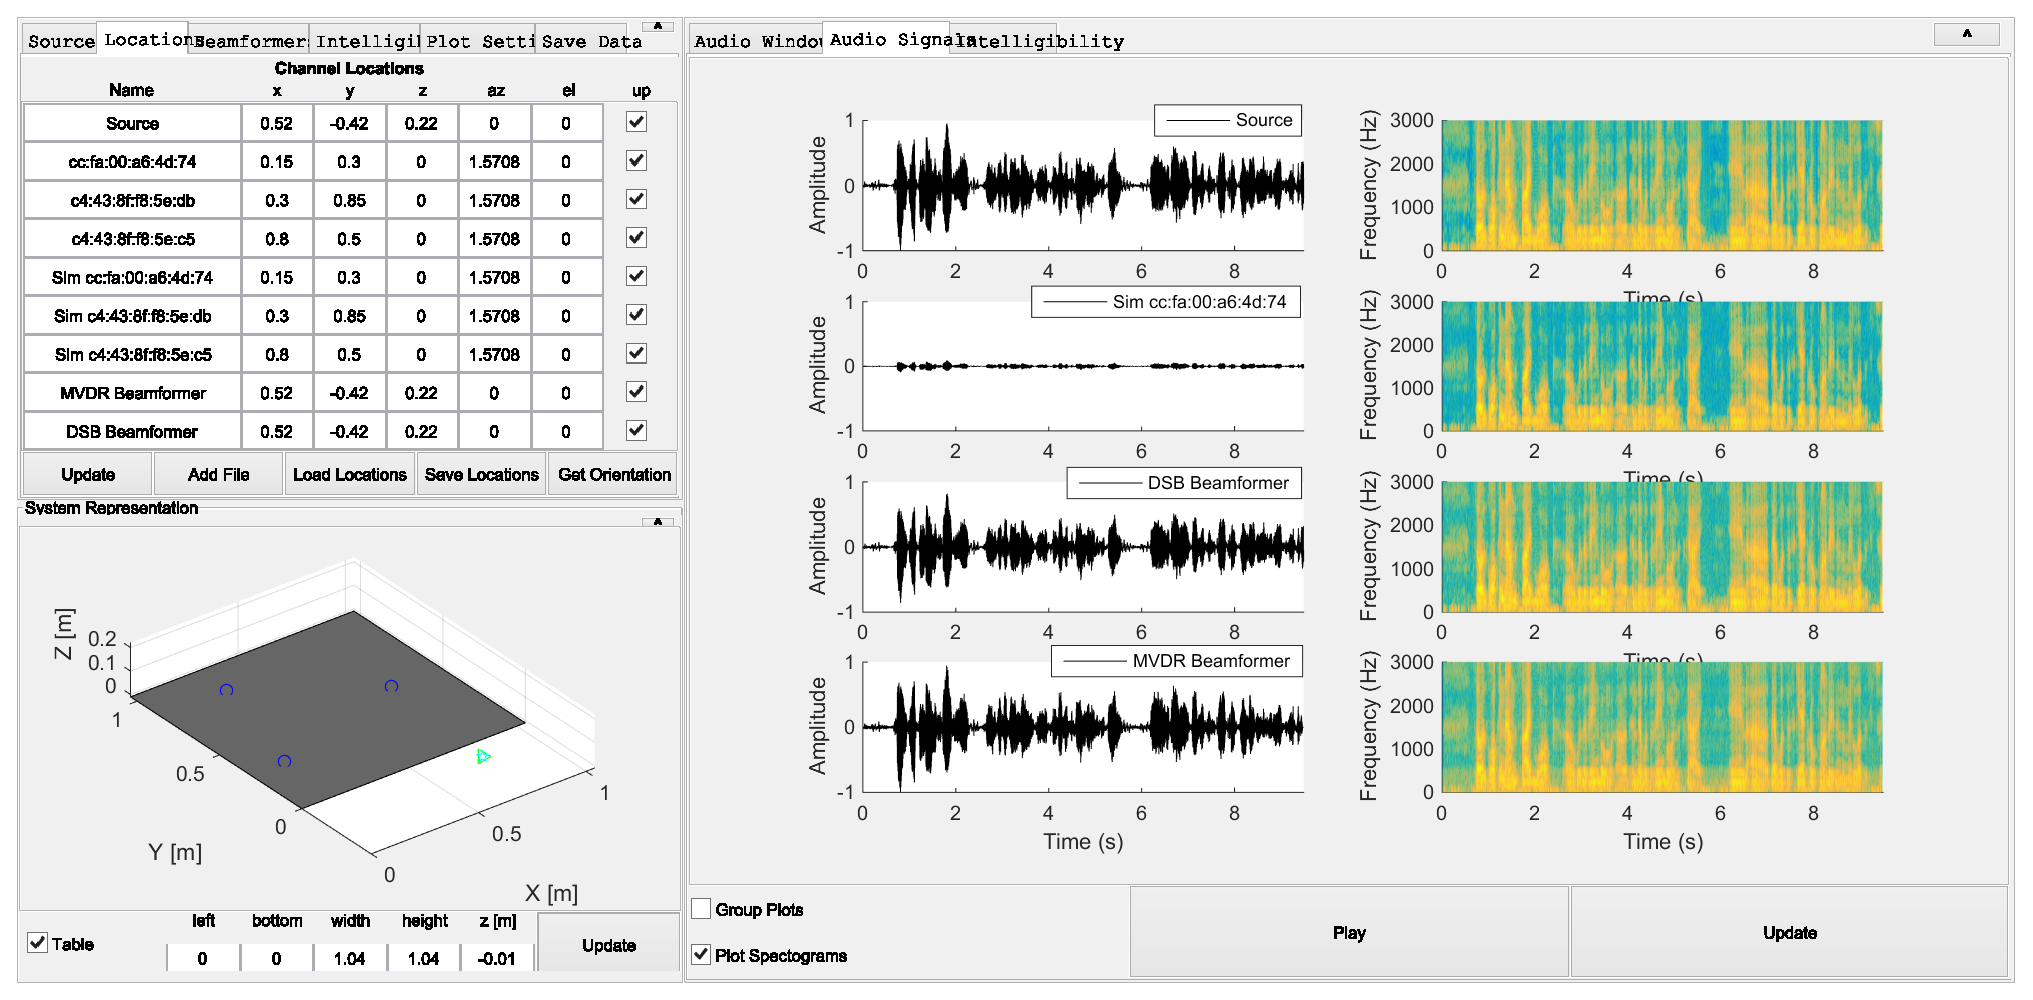
\includegraphics[width = \columnwidth]{GUI_screenshot.eps} % l b r t
    \caption[User interface implemented in \matlab]{Matlab Realtime Beamforming Toolbox GUI}
    \label{fig:GUI}
\end{figure}

\subsection{User Interface (UI)}
\label{sec:des_realtime}
The UI has been build with a modular design. Every UI panel can run individually, or they can be connected with a main object that has multiple UI panels. There is a panel where frames from the buffer can be plotted in realtime and one where the whole channel can be plotted. These can also be used to easily playback (part of) the data and to plot the frequency spectrum against time. There is a panel where the intelligibility metric outputs are shown. Each of the inputs has its own panel with buttons to start or stop streaming or several others. There is a panel which can be used to save data to multiple audio formats, with the locations stored in the meta-data of the audio file, or as \matlab .mat files, with all relevant labels saved. Each of the beamformers has a panel to change their parameters and to enable them, or to process data at once. The intelligibility metrics have a similar panel and a separate panel where the metrics are shown, and the output of the $SNR$ algorithm is plotted against time. There is a standard selector panel which is used in multiple places to connect inputs to processing units. All the locations can be entered in the locations panel. Lastly there is a system representation tab which plots the locations of the channels in the buffer on an axis and can also draw a tabletop surface. This makes it easy to compare modeled scenario with the real scenario.

\chapter{Results}
\label{chap:results}

There are two implemented MVDR algorithms, one assuming uniform microphone directivity and one including the directivities of the used microphones. Comparing these two gives an indication of what the influence of including the directivities are, since the directivities are the only difference between the two algorithms. It is expected that compensating for these directivities should lead to an increase in performance of the beamforming algorithm. This section covers the results of these experiments and simulations. These results are put in tables to give a clear overview of the results. 

\section{Measurement Scenario}

% \vspace{\baselineskip}
A set of experiments have been done to demonstrate the effect of the different beamformers on recorded audio. Experiments excluding and including the directivities of the microphones have been done to determine the impact including directivities has on the beamforming algorithms. In this research, the DSB, the MVDR beamformer excluding directivities and the MVDR beamformer including directivities have been investigated. 

There are two kinds of experiments conducted. The first are measurements were done in the anechoic chamber in the applied physics building at TU Delft. The other experiments are performed in an office room with dimensions $6.60m$ x $3.90m$ x $3.15m$, $[x,y,z]$.


\subsection{Anechoic Chamber experiments}

Measurements have been done in the anechoic chamber to measure recorded audio without the presence of reverberations. Two Speakers and three smartphones were used during these measurements, as illustrated in figure \ref{fig:anechoic_setup}. In this figure, the distances between the different objects are given.

\begin{figure}[h!]
	\centering  
	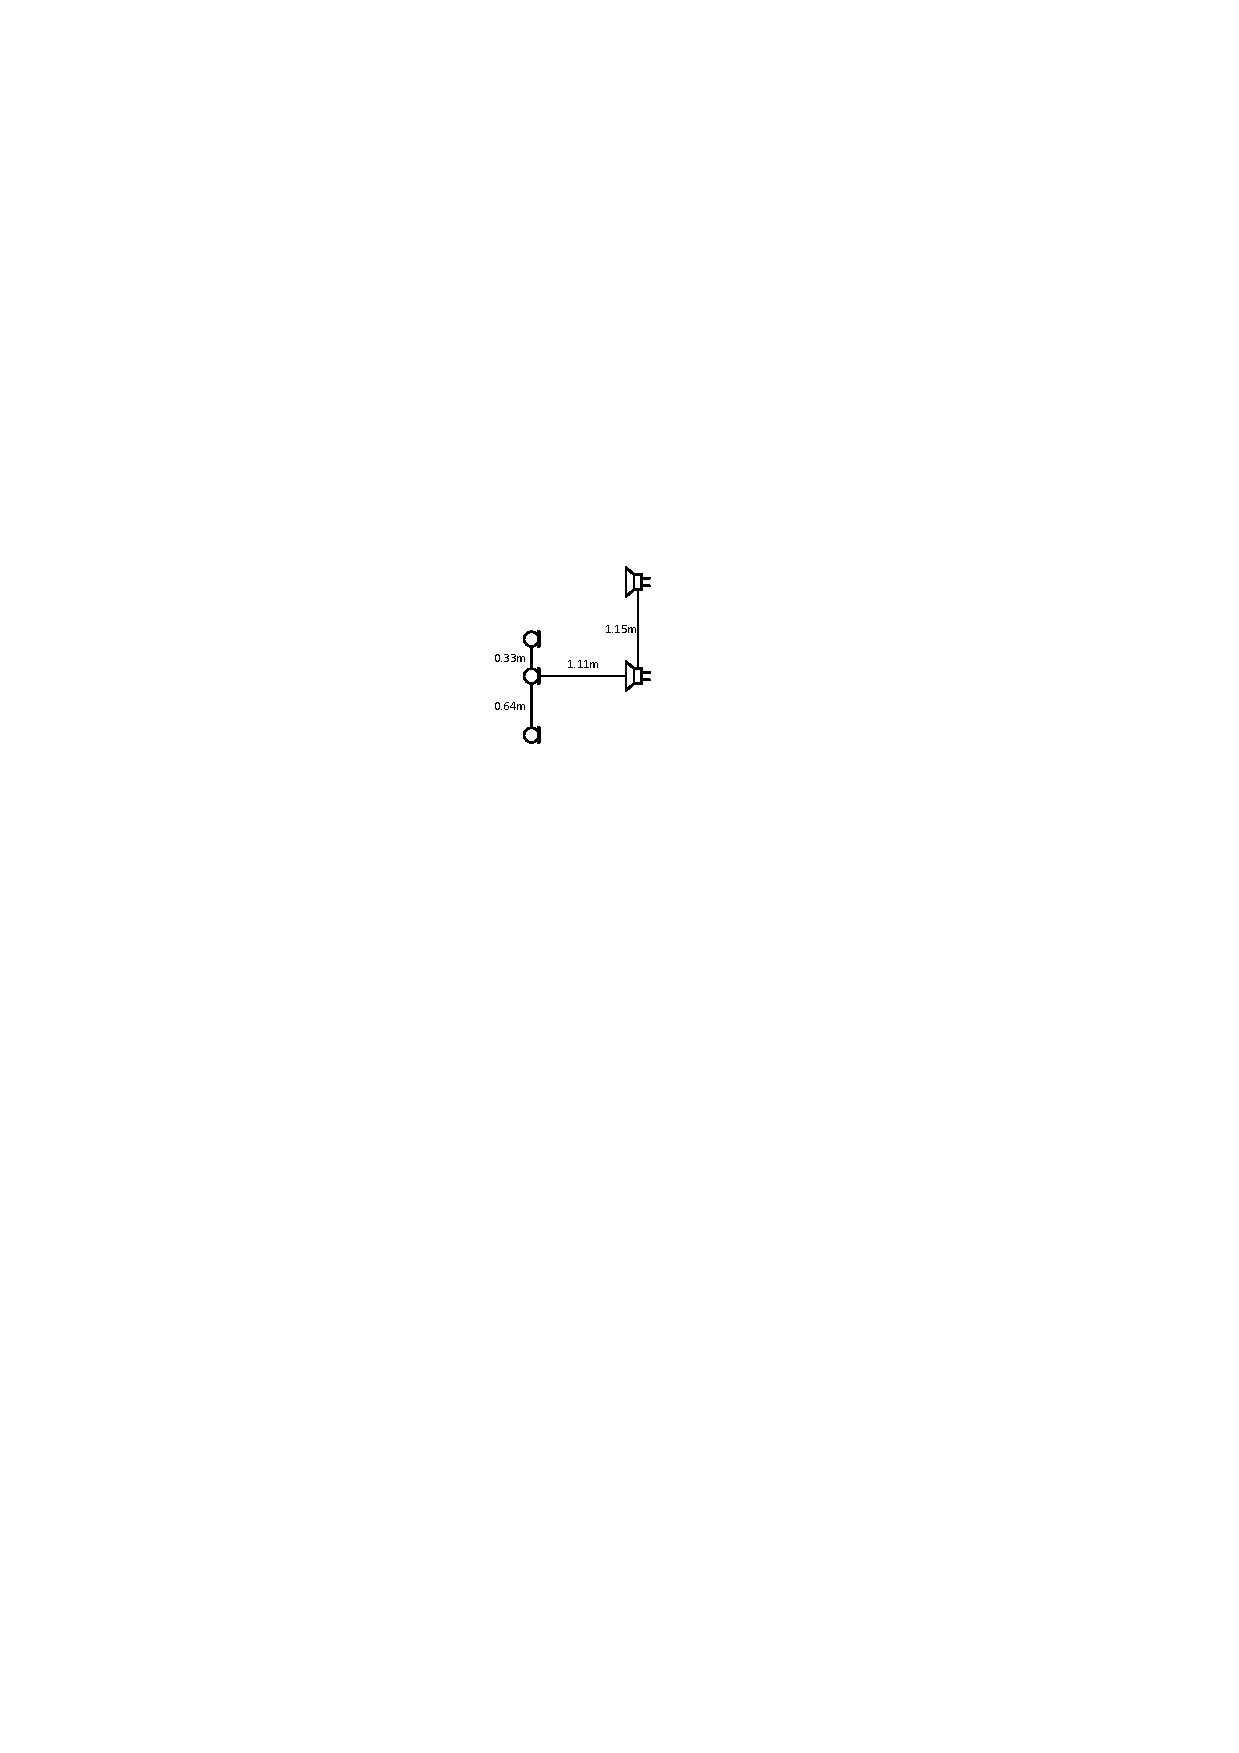
\includegraphics[scale=1.5, clip=true, trim = 8.25cm 17cm 10cm 9.5cm] {anechoic_setup.pdf} % l b r t]
	\caption[Setup of the measurements in the anechoic room]{Anechoic setup} 
	\label{fig:anechoic_setup}
\end{figure}

Beamforming has been performed on the recorded audio to determine the performance of the beamforming algorithms in a real room without reverberations. De audio signals and spectrograms of the source, the closest microphone and the different beamforming algorithms have been plotted in \ref{fig:anechoic_results}.
\begin{figure}[h!]
	\centering  
	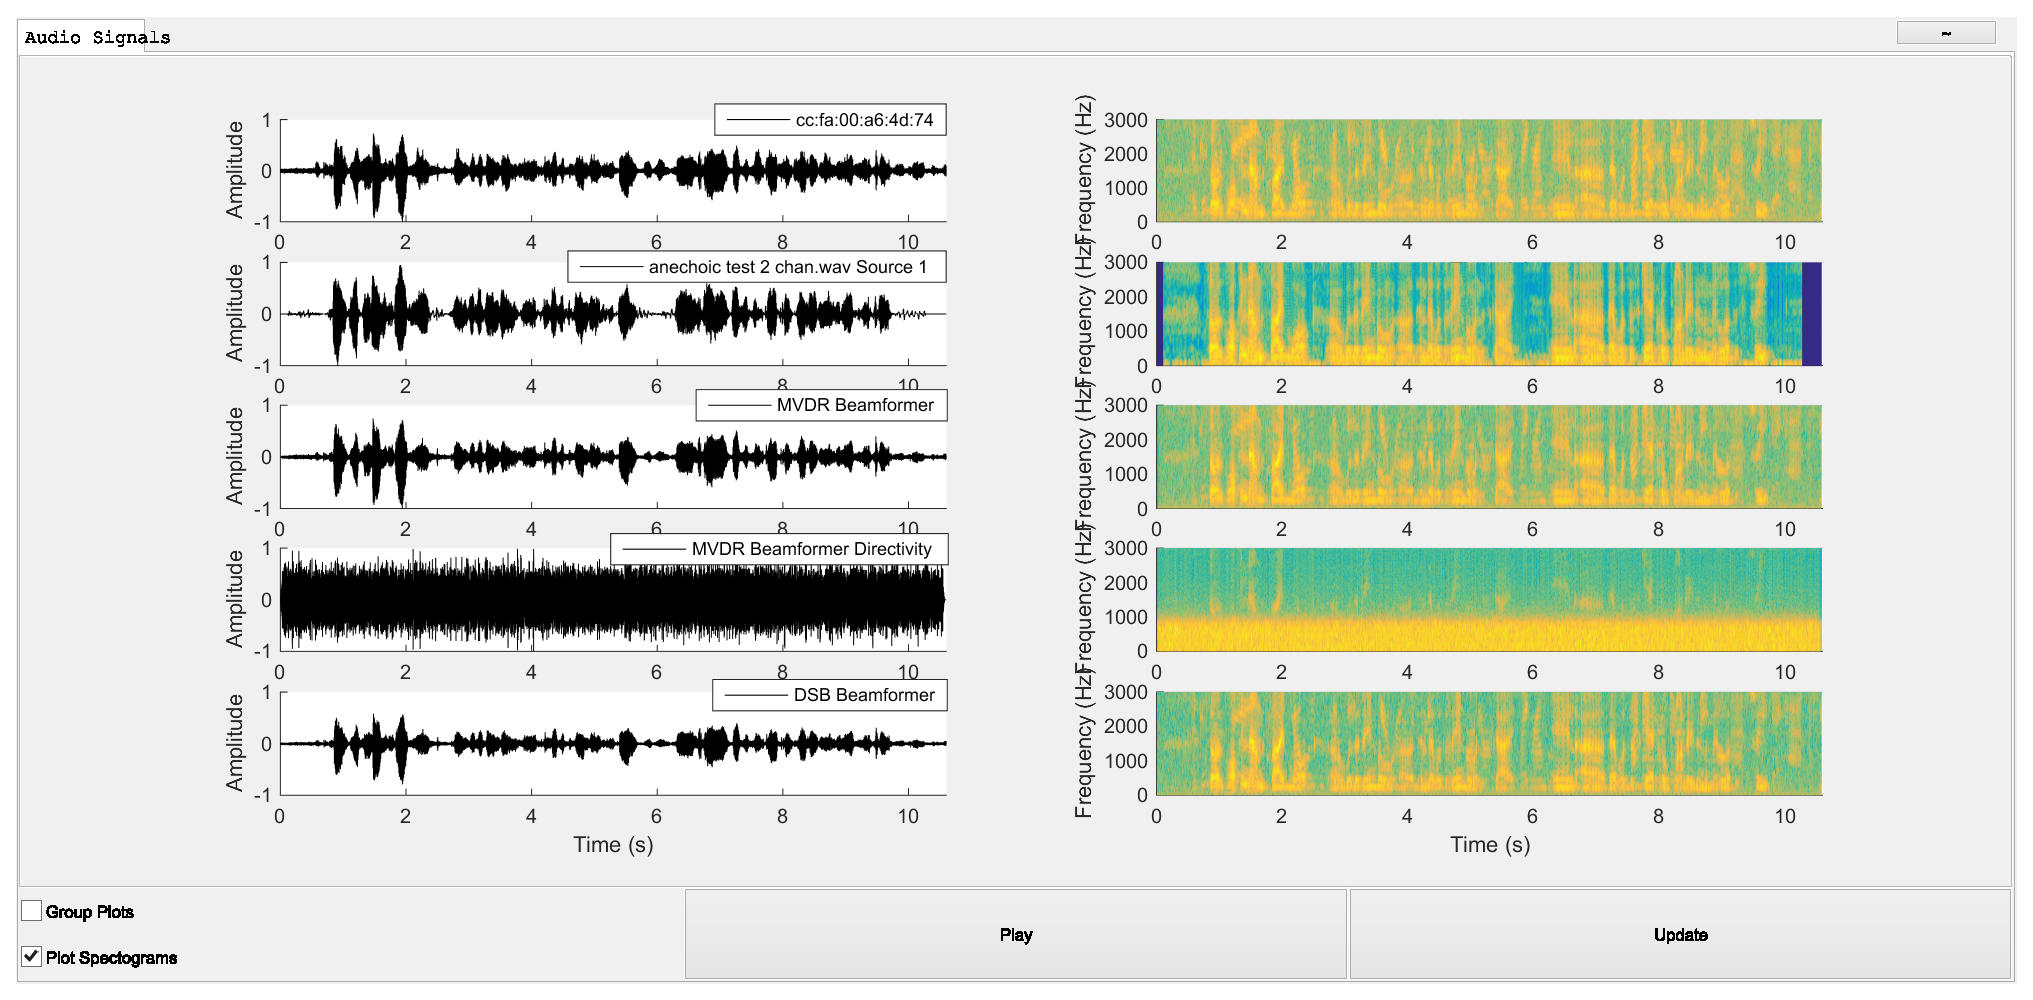
\includegraphics[width = 0.9\columnwidth] {plot_anechoic_results_with_spectogram} % l b r t]
	\caption[Audio signals and spectrogram anechoic chamber experiment 1: With an interfering audio source]{Audio signals and spectrogram anechoic chamber experiment 1: With an interfering audio source} 
	\label{fig:anechoic_results}
\end{figure}

These audio signals are used to calculate the intelligibility measures. The results of these intelligibility calculation are plotted in \ref{fig:anechoic_intelligibility} 

\begin{figure}[h!]
	\centering  
	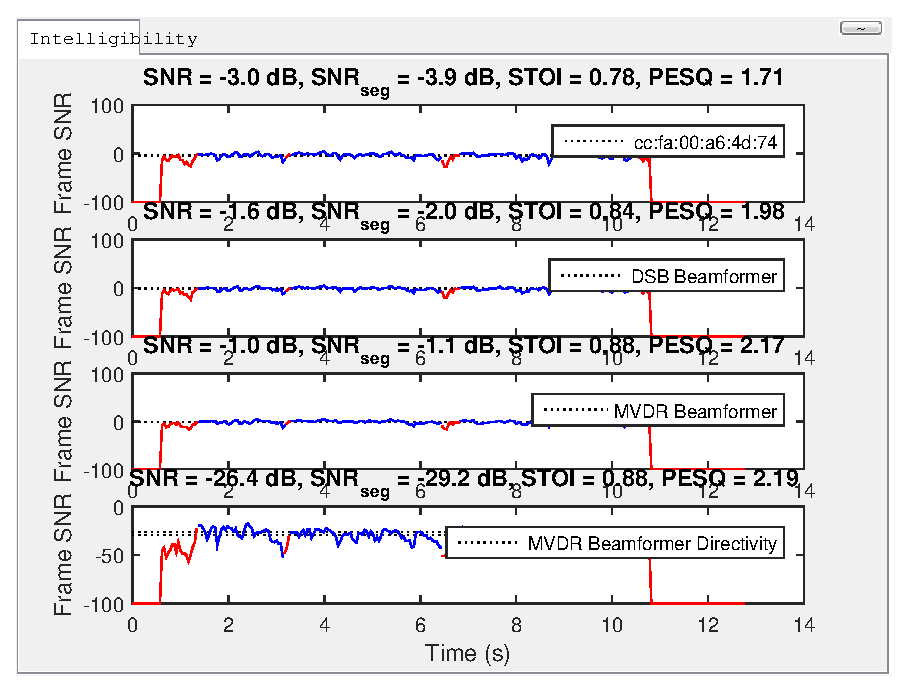
\includegraphics[width = 0.8\columnwidth] {Screenshots_experimenten/Intelligibility/anechoic} % l b r t]
	\caption[Intelligibility anechoic chamber experiment 1: With an interfering audio source]{Intelligibility anechoic chamber experiment 1: With an interfering audio source} 
	\label{fig:anechoic_intelligibility}
\end{figure}

Finally the results have been put in table \ref{tab:anechoic_res}. The results have also been put in table \ref{tab:expRes}, which is a large table at the end of the chapter with the anechoic chamber results as well as results from office room experiments. This table makes the different experimental results easily comparable.

\newpage

\begin{table}[h]
\centering
\begin{tabular}{|c|c|c|c|c|} \hline
								
								& \multicolumn{4}{c|}{Anechoic measurement} \\ \hline
								
Beamformer						& Closest  	& DSB 	& MVDR 	& MVDR+ 	\\ \hline
														
Performance measure 			&			&		&		&			\\
																						
SNR 							& -3.0		& -1.6	& -1.0	& -26.4		  \\
																						
$\text{SNR}_\text{seg}$ 		& -3.9		& -2.0	& -1.1	& -29.2		  \\
																						
STOI    						& 0.78		& 0.84	& 0.88	& 0.88		  \\
																					
PESQ  							& 1.71		& 1.98	& 2.17	& 2.19		  \\
																
White noise gain 				&			& -4.65	& 56.85	& 102.05		 \\ \hline

\end{tabular}
\caption{Experimental results of the anechoic chamber measurement}
\label{tab:anechoic_res}
\end{table}




\subsection{Office room experiments}
During the office room experiments the sound is recorded with a sampling frequency of $48000 Hz$ by smartphone microphones. This sound is used to perform the beamforming algorithms on. 

During the office room experiments, the following procedure has been followed:

\begin{itemize}
\item 2 speakers were placed at known locations with English voices, one as interference and one as source.
\item 3 smartphones placed at known locations with known orientations.
\item Both speakers played audio of english voices at the same time.
\item The smartphones streamed the audio data to the \matlab toolbox where it was recorded and synchronized.
\end{itemize}

This configuration is illustrated in figure \ref{fig:configuration}.

\begin{figure} [h!]
	\centering  
	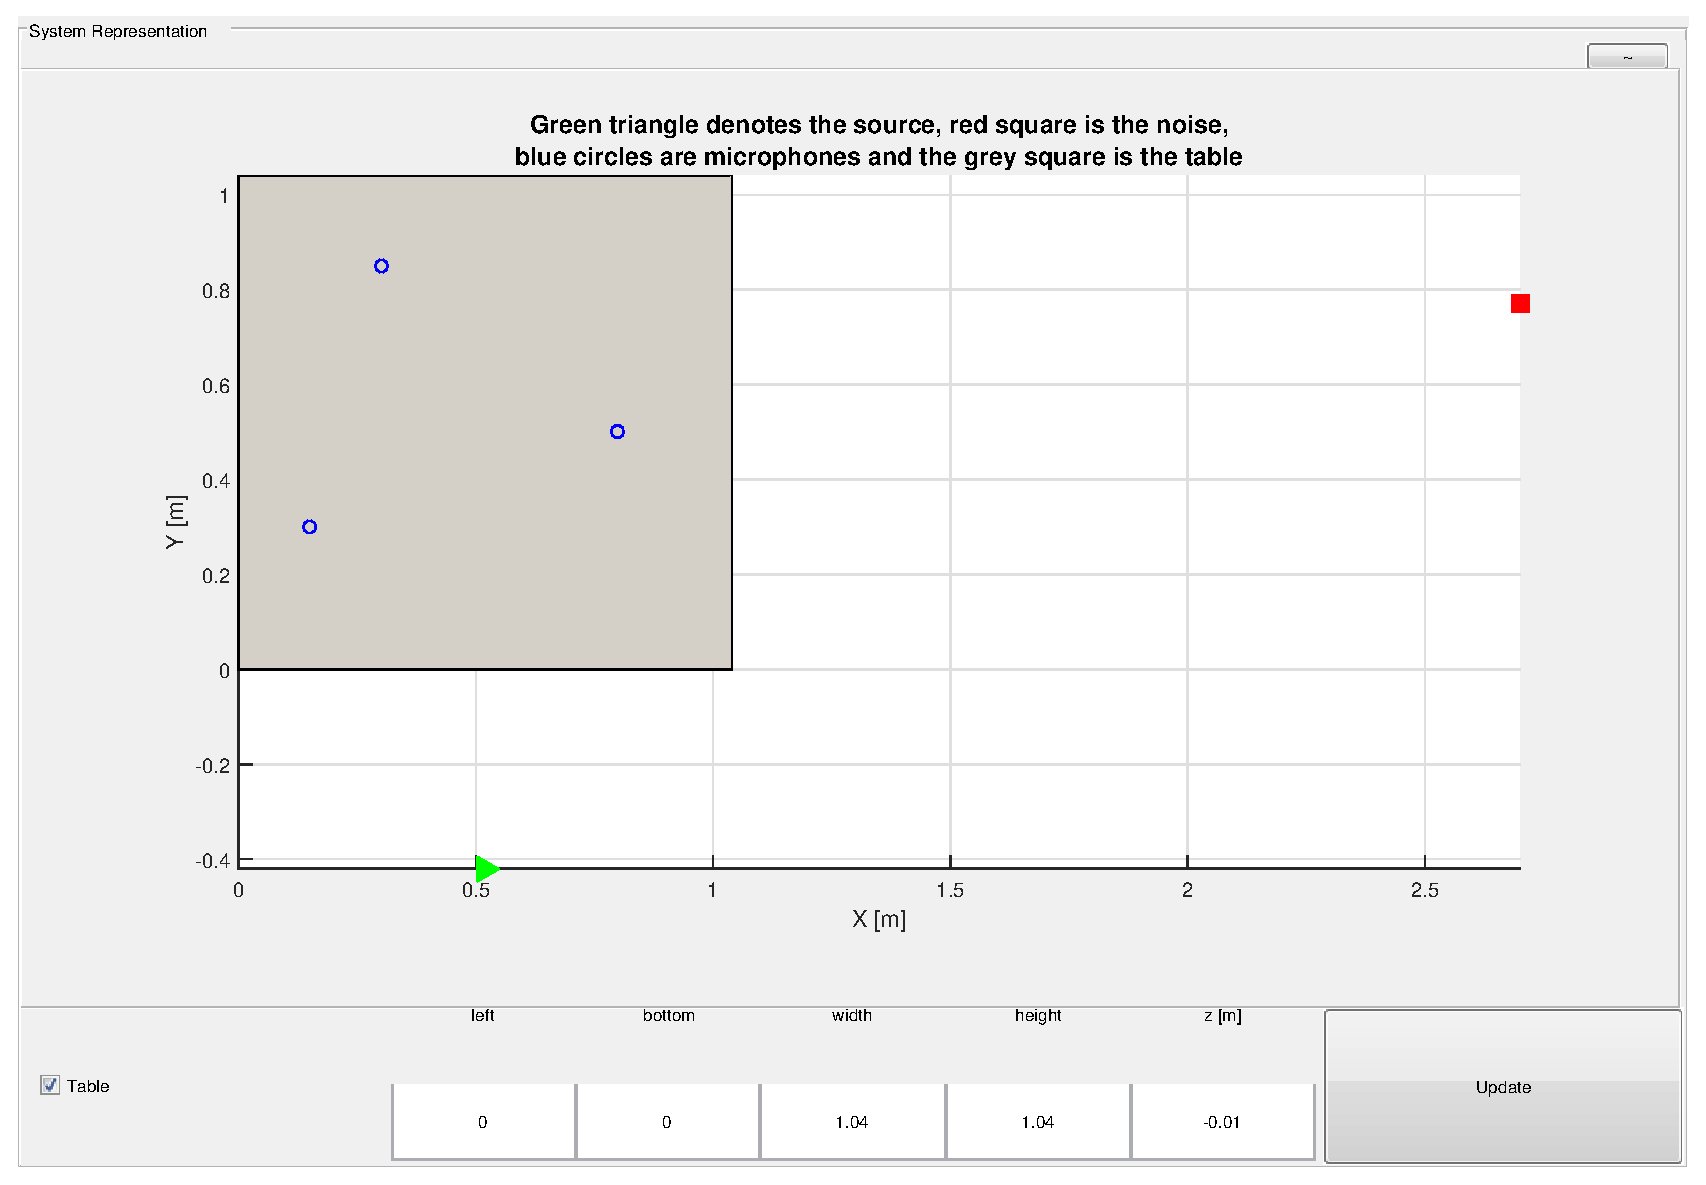
\includegraphics[scale=0.5, clip=true, trim = 2.0cm 3.5cm 1cm 1.5cm] {system_representation.eps} % l b r t]
	\caption[System configuration during the office room experiments]{Office room experiment configuration. Microphone Locations: $(0.15,0.3 , 0)$, $(0.8 , 0.5 , 0)$, $(0.3 , 0.85 , 0)$, Source Location: $(0.52 , -0.42 , 0.22)$, Interferer Location: $(2.7 , 0.77 , -0.2)$} 
	\label{fig:configuration}
\end{figure}


\subsection{Simulations of the office room experiments}

Simulations of the same microphone setup as during the office room experiments have been done to see how much the conducted experiments differ from these simulated scenario. During the simulations, the parameters as described in section \ref{sec:des_simulation} have been varied to investigate the sensitivity of the beamforming algorithms to each of the parameters. The simulated scenarios are as follows:

\newpage

\begin{table}[h!]
\centering
\begin{tabular}{|c|c|c|c|} \hline
Simulation 		& reverberations 		& Added white noise at SNR [dB] 	& Standard deviation of position errors \\ \hline
1 				& Excluded  			& 60						 		& 0 \\
2 				& Included 				& 60						 		& 0 \\
3 				& Excluded  			& 40						 		& 0 \\
4 				& Included 				& 40						 		& 0 \\
5 				& Excluded 				& 60						 		& 0.05 \\
6 				& Included  			& 60						 		& 0.05 \\ \hline
\end{tabular}
\caption{The simulated scenarios}
\label{tab:sim_scenarios}
\end{table}

A perfect match cannot be expected since the simulated microphones are omnidirectional which is not the case for smartphone microphones. However, These simulations can determine if the beamforming algorithms perform in a simulated scenario and how sensitive the beamformers are to the different parameters.

For both the DSB and MVDR beamformer, the results of the simulations are put in table \ref{tab:simRes}. For the fifth and sixth simulation, the SNR of the closest microphone has a negative value (in decibels). In this case, it is not representative for the performance of the beamformer to use the array-gain. This is because a positive SNR after a beamforming algorithm results in a negative array-gain and, in general, a negative array-gain indicates a poor performing beamforming algorithm. Therefore the entries in the table for the array gain are left blank for both these simulations.

\subsection{Results of the office room experiment}

During the conducted office room experiments, the orientation of the microphones have been varied for the microphone setup earlier illustrated in fig \ref{fig:configuration}. The investigated orientations are :

\begin{itemize}
\item $\theta = -90\degree$ (microphones facing the source)
\item $\theta = 0\degree$ (microphones facing the interfering sound source)
\item $\theta = 90\degree$ (microphones directed away from the source
\item Each microphone in a different orientation.
\end{itemize}

Where $\theta = 0\degree$ is taken in the direction of the positive x-axis and the angle increases in the counterclockwise direction. In the remainder of this section, the microphone locations are denoted by their (x,y,z) location as illustrated in figure \ref{fig:configuration}. 

A scenario with different orientations was investigated since the aim of this thesis was to research beamforming algorithms with ad-hoc microphone arrays. The orientations of the microphones in an ad-hoc microphone array will also be different for each microphone. During this experiment, the microphone located at (0.3,0.85,0) was orientated at $\theta = -90\degree$, the microphone located at (0.8,0.5,0) was orientated at $\theta = 0\degree$ and the microphone located at (0.15,0.3,0) was oriented $\theta = 90\degree$. 

The last office room experiment that has been conducted was with a linear array to compare the results of this array to the earlier ad-hoc arrays. The different microphones were located at different  with the same y-coordinate. To be exact, the locations of the microphones were (0.27,0.75,0), (0.52,0.75,0), (0.77,0.75,0).

The office room experiments were once conducted with only the source speaker playing an English voice and once with the source speaker and noise speaker playing English voices. The different performance measures as presented in section \ref{sec:des_evaluation} are calculated for each of the three beamforming algorithms and for the closest microphone. The performance measures of the closest microphone will be used to determine if and how much the signal is enhanced by the beamforming algorithms. With these results it is also possible to compare the result of each beamformimg algorithm and conclude which beamforming algorithm has the best performance. The results of the office room experiments are put in table \ref{tab:expRes}. In this table, MVDR is the standard MVDR algorithm and MVDR+ stands for the MVDR beamforming algorithm with the compensation for the directional gain of the microphones included. The SNR of the closest microphones in each of the cases is negative (in decibels) and therefore the array-gain will not give a good indication about the performance of the beamforming algorithms. For this reason, the array-gain is left out of this table.



% Simulated results
\begin{sidewaystable}[h]
\centering

\caption{Simulated results}
\label{tab:simRes}
  \begin{adjustbox}{max width=\textwidth}
\begin{tabular}{|c|c|c|c|c|c|c|c|c|c|c|c|c|c|c|c|c|}
\hline
%\multicolumn{10}{|c|}{\multirow{2}{*}{With an interfering audio source}} \\ 
%\multicolumn{10}{|l|}{} \\ \hline

 & \multicolumn{3}{c|}{Simulation 1}					& \multicolumn{3}{c|}{Simulation 2} 					& \multicolumn{3}{c|}{Simulation 3} 					\\ 
 & \multicolumn{3}{c|}{Without reverberations}			& \multicolumn{3}{c|}{With reverberations} 				& \multicolumn{3}{c|}{Without reverberations} 			\\ 
 & \multicolumn{3}{c|}{White noise added at 60dB SNR}	& \multicolumn{3}{c|}{White noise added at 60dB SNR} 	& \multicolumn{3}{c|}{White noise added at 40dB SNR} 	\\
 & \multicolumn{3}{c|}{Without position errors}			& \multicolumn{3}{c|}{Without position errors}			& \multicolumn{3}{c|}{Without position errors} 			\\ \hline
 
Beamformer				& Closest  	& DSB 		& MVDR 	& Closest  	& DSB 	& MVDR 	& Closest  	& DSB 	& MVDR \\ \hline

Performance measure 	& 	 		& 	 		& 	 	& 	 	& 		& 		&     &   	 & \\

SNR 					& 6.2		& 12.6		& 34.7 	& 2.9 	& 8.2 	& 8.6 	& 5.2 & 11.6 & 17.1 \\

$\text{SNR}_\text{seg}$	& 4.8		& 10.1		& 28.7 	& -1.3 	& 3.5 	& 5.6 	& 1.5 & 7.5 & 11.4 \\

STOI    				& 0.80		& 0.90		& 0.99 	& 0.77 	& 0.88 	& 0.95 	& 0.78 & 0.89 & 0.93 \\

PESQ  					& 1.82		& 2.29		& 3.66 	& 1.83 	& 2.16 	& 2.92 	& 1.65 & 2.09 & 2.28 \\

Array gain  			& 			& 2.03		& 5.61 	&  		& 2.78 	& 2.93 	& 	 	& 2.22 & 3.27 \\

White noise gain 		& 			& -4.64		& 51.92 & 	 	& -4.64 & 52.69 & 	 	& -4.64 & 50.94  \\ \hline \hline




 & \multicolumn{3}{c|}{Simulation 4} & \multicolumn{3}{c|}{Simulation 5} & \multicolumn{3}{c|}{Simulation 6} \\
 & \multicolumn{3}{c|}{With reverberations}				& \multicolumn{3}{c|}{Without reverberations} 						& \multicolumn{3}{c|}{With reverberations} 									\\ 
 & \multicolumn{3}{c|}{White noise added at 40dB SNR}	& \multicolumn{3}{c|}{White noise added at 60dB SNR} 				& \multicolumn{3}{c|}{White noise added at 60dB SNR} 						\\
 & \multicolumn{3}{c|}{Without position errors}			& \multicolumn{3}{c|}{with position errors with a sigma of 0.05}	& \multicolumn{3}{c|}{with position errors with a sigma of 0.05} 			\\ \hline
 
Beamformer				& Closest  	& DSB 	& MVDR 	& Closest  	& DSB 	& MVDR 	& Closest  	& DSB 	& MVDR \\ \hline

Performance measure 	& 			& 		&  		&  			&  		&  		&  			&  		& 		\\
						
SNR 					& 2.5		& 7.8	& 9.5 	& -2.4 		& 1.6 	& -2.3 	& -3.3 		& -0.1 	&  -0.6 \\
							
$\text{SNR}_\text{seg}$	& -2.1		& 3.0	& 4.9 	& -6.3 		& -3.0	& -6.5 	& -7.3 		& -4.5 	&  -3.3 \\
							
STOI    				& 0.75		& 0.87	& 0.91	& 0.68 		& 0.79 	& 0.85 	& 0.70 		& 0.76 	& 0.86 \\
							
PESQ  					& 1.66		& 2.00	& 2.25 	& 1.55 		& 1.91 	& 2.41 	& 1.75 		& 1.71 	& 2.50 \\
							
Array gain  			& 			& 3.19	& 3.88 	&  			& -0.64	& 0.94	&  			& 		&  		\\
							
White noise gain 		& 			& -4.64	& 50.96	&  			& -4.63	& 50.93	&  			& -4.64 & 51.05 \\


\hline
\end{tabular}
\end{adjustbox}
\end{sidewaystable}







% Experimental results
\begin{sidewaystable}[h]
\centering

\caption{Experimental results}
\label{tab:expRes}
  \begin{adjustbox}{max width=\textwidth}
\begin{tabular}{|c|c|c|c|c|c|c|c|c|c|c|c|c|c|c|c|c|}
\hline
\multicolumn{13}{|c|}{\multirow{2}{*}{Without an interfering audio source}} \\ 
\multicolumn{13}{|c|}{} \\ \hline

						& \multicolumn{4}{c|}{$\theta = -90\degree$}	& \multicolumn{4}{c|}{$\theta = 0\degree$} 	& \multicolumn{4}{c|}{$\theta = -90\degree$} \\ \hline
	
Beamformer				& Closest  	& DSB 	& MVDR 	& MVDR+ 		& Closest  	& DSB 	& MVDR 	& MVDR+ 		& Closest  	& DSB 	& MVDR 	& MVDR+ \\ \hline
				
Performance measure 	& 			& 		&   	&   			& 	 		&   	& 	 	&   			& 			& 		&  		&  \\
				
SNR 					& -6.5		& -5.9	& -9.4 	& -32.1 		& -6.7 		& -6.2 	& -14.3 & -47.3 		& -6.5		& -5.8	& -9.5 	& -33.3 \\
						
$\text{SNR}_\text{seg}$	& -3.0		& -1.8	& -6.4 	& -31.7 		& -7.0 		& -6.0 	& -15.5 & -49.9 		& -6.6		& -5.4	& -10.7	& -35.9 \\
						
STOI   					& 0.73		& 0.81	& 0.73	& 0.74 			& 0.71 		& 0.76 	& 0.50 	& 0.51  		& 0.71		& 0.76	& 0.58 	& 0.57 	\\
						
PESQ  					& 2.45		& 2.68	& 2.18 	& 2.24 			& 2.34 		& 2.53 	& 1.47 	& 1.55  		& 2.36		& 2.54	& 1.78 	& 1.74	\\
						
White noise gain 		& 			& -4.64	& 50.99 & 105.06 		&   		& -4.63 & 52.24 & 96.59 		& 			& -4.64	& 52.21 & 93.80 \\ \hline

						& \multicolumn{4}{c|}{Different orientations}& \multicolumn{4}{c|}{Linear array}  		\\ \cline{1-9}

Beamformer				& Closest  	& DSB 	& MVDR 	& MVDR+ 		& Closest  	& DSB 	& MVDR 		& MVDR+ 	\\ \cline{1-9}
	
Performance measure 	&  			&  		&  		&  				&  			&  		&  			&  			\\
	
SNR 					& -6.4 		& -5.8 	& -9.8 	& -34.7 		& -7.1 		& -8.6 	& -13.0 	& -55.3 	\\
									
$\text{SNR}_\text{seg}$	& -6.3 		& -5.2 	& -10.8 & -37.3 		& -7.0 		& -11.0 & -14.1 	& -57.9 	\\
			
STOI    				& 0.70 		& 0.78 	& 0.58 	& 0.58 			& -13.0 	& 0.51 	& 0.47 		& 0.48 		\\
										
PESQ  					& 2.36 		& 2.59 	& 1.71 	& 1.74 			& -55.3 	& 2.04 	& 1.53 		& 1.70 		\\
	
White noise gain 		&  			& -4.64 & 52.66 & 96.19 		&  			& -4.77 & 54.08 	& 105.10 	\\

\hline \hline 
\multicolumn{13}{|c|}{\multirow{2}{*}{With an interfering audio source}} \\ 
\multicolumn{13}{|l|}{} \\ \hline

						& \multicolumn{4}{c|}{$\theta = -90\degree$} 	& \multicolumn{4}{c|}{$\theta = 0\degree$} 	& \multicolumn{4}{c|}{$\theta = 90\degree$} \\ \hline

Beamformer				& Closest  	& DSB 	& MVDR 	& MVDR+ 		& Closest  	& DSB 	& MVDR 	& MVDR+ 		& Closest  	& DSB 	& MVDR 	& MVDR+  \\ \hline

Performance measure 	& 			& 		&  		&  				&  			&  		&  		&  				&	  		&  		&  		& \\ 

SNR 					& -6.8 & -5.8 & -7.0 & -29.9 & -7.3 & -6.3 & -8.9 & -31.2 & -6.7	& -6.5	& -13.8 & -53 \\ 

$\text{SNR}_\text{seg}$	& -6.7 & -5.0 & -7.8 & -32.5 & -7.8 & -6.1 & -9.7 & -33.8 & -7.3	& -7.6	& -15.7 & -55.6 \\

STOI    				& 0.70 & 0.79 & 0.64 & 0.65 & 0.66 & 0.72 & 0.56 & 0.58 & 0.65	& 0.65	& 0.48 & 0.47 	\\

PESQ  					& 2.32 & 2.54 & 1.81 & 1.89 & 2.10 & 2.37 & 1.72 & 1.83 & 2.06	& 1.97	& 1.29 & 1.39 	\\

White noise gain 		&  	  & -4.64 & 52.82 & 105.08 &   & -4.64 & 52.33 & 96.53 &  		& -4.64	& 51.96 & 93.82 \\ \hline

						& \multicolumn{4}{c|}{Different orientations}& \multicolumn{4}{c|}{Linear array} 	& \multicolumn{4}{c|}{Anechoic measurement} \\ \hline

Beamformer				& Closest  	& DSB 	& MVDR 	& MVDR+ 		& Closest  	& DSB 	& MVDR 	& MVDR+ 	& Closest  	& DSB 	& MVDR 	& MVDR+ 	\\ \hline

Performance measure 	&  			&  		&  		&  				&  			&  		&  		&  			&			&		&		&			\\

SNR 					& -6.8		& -6.0 	& -7.9 	& -28.5 		& -7.1		& -6.2	& -7.2 	& -34.1 	& -3.0		& -1.6	& -1.0	& -26.4		  \\
								
$\text{SNR}_\text{seg}$ & -7.5		& -5.9 	& -8.8 	& -31.1 		& -7.6		& -6.2	& -8.1 	& -36.7 	& -3.9		& -2.0	& -1.1	& -29.2		  \\
								
STOI    				& 0.64		& 0.73 	& 0.58 	& 0.60 			& 0.67		& 0.70	& 0.53 	& 0.54 		& 0.78		& 0.84	& 0.88	& 0.88		  \\
								
PESQ  					& 2.08		& 2.36 	& 1.72 	& 1.81 			& 2.12 		& 2.30	& 1.68 	& 1.80 		& 1.71		& 1.98	& 2.17	& 2.19		  \\
					
White noise gain 		& 			& -4.64 & 52.24 & 98.88 		&  			& -4.77 & 54.56 & 104.99  	&			& -4.65	& 56.85	& 102.05		 \\

\hline
\end{tabular}
\end{adjustbox}
\end{sidewaystable}





% Oude tabellen

%\begin{figure} [h!]
%	\minipage{0.32\textwidth}
%		\fbox{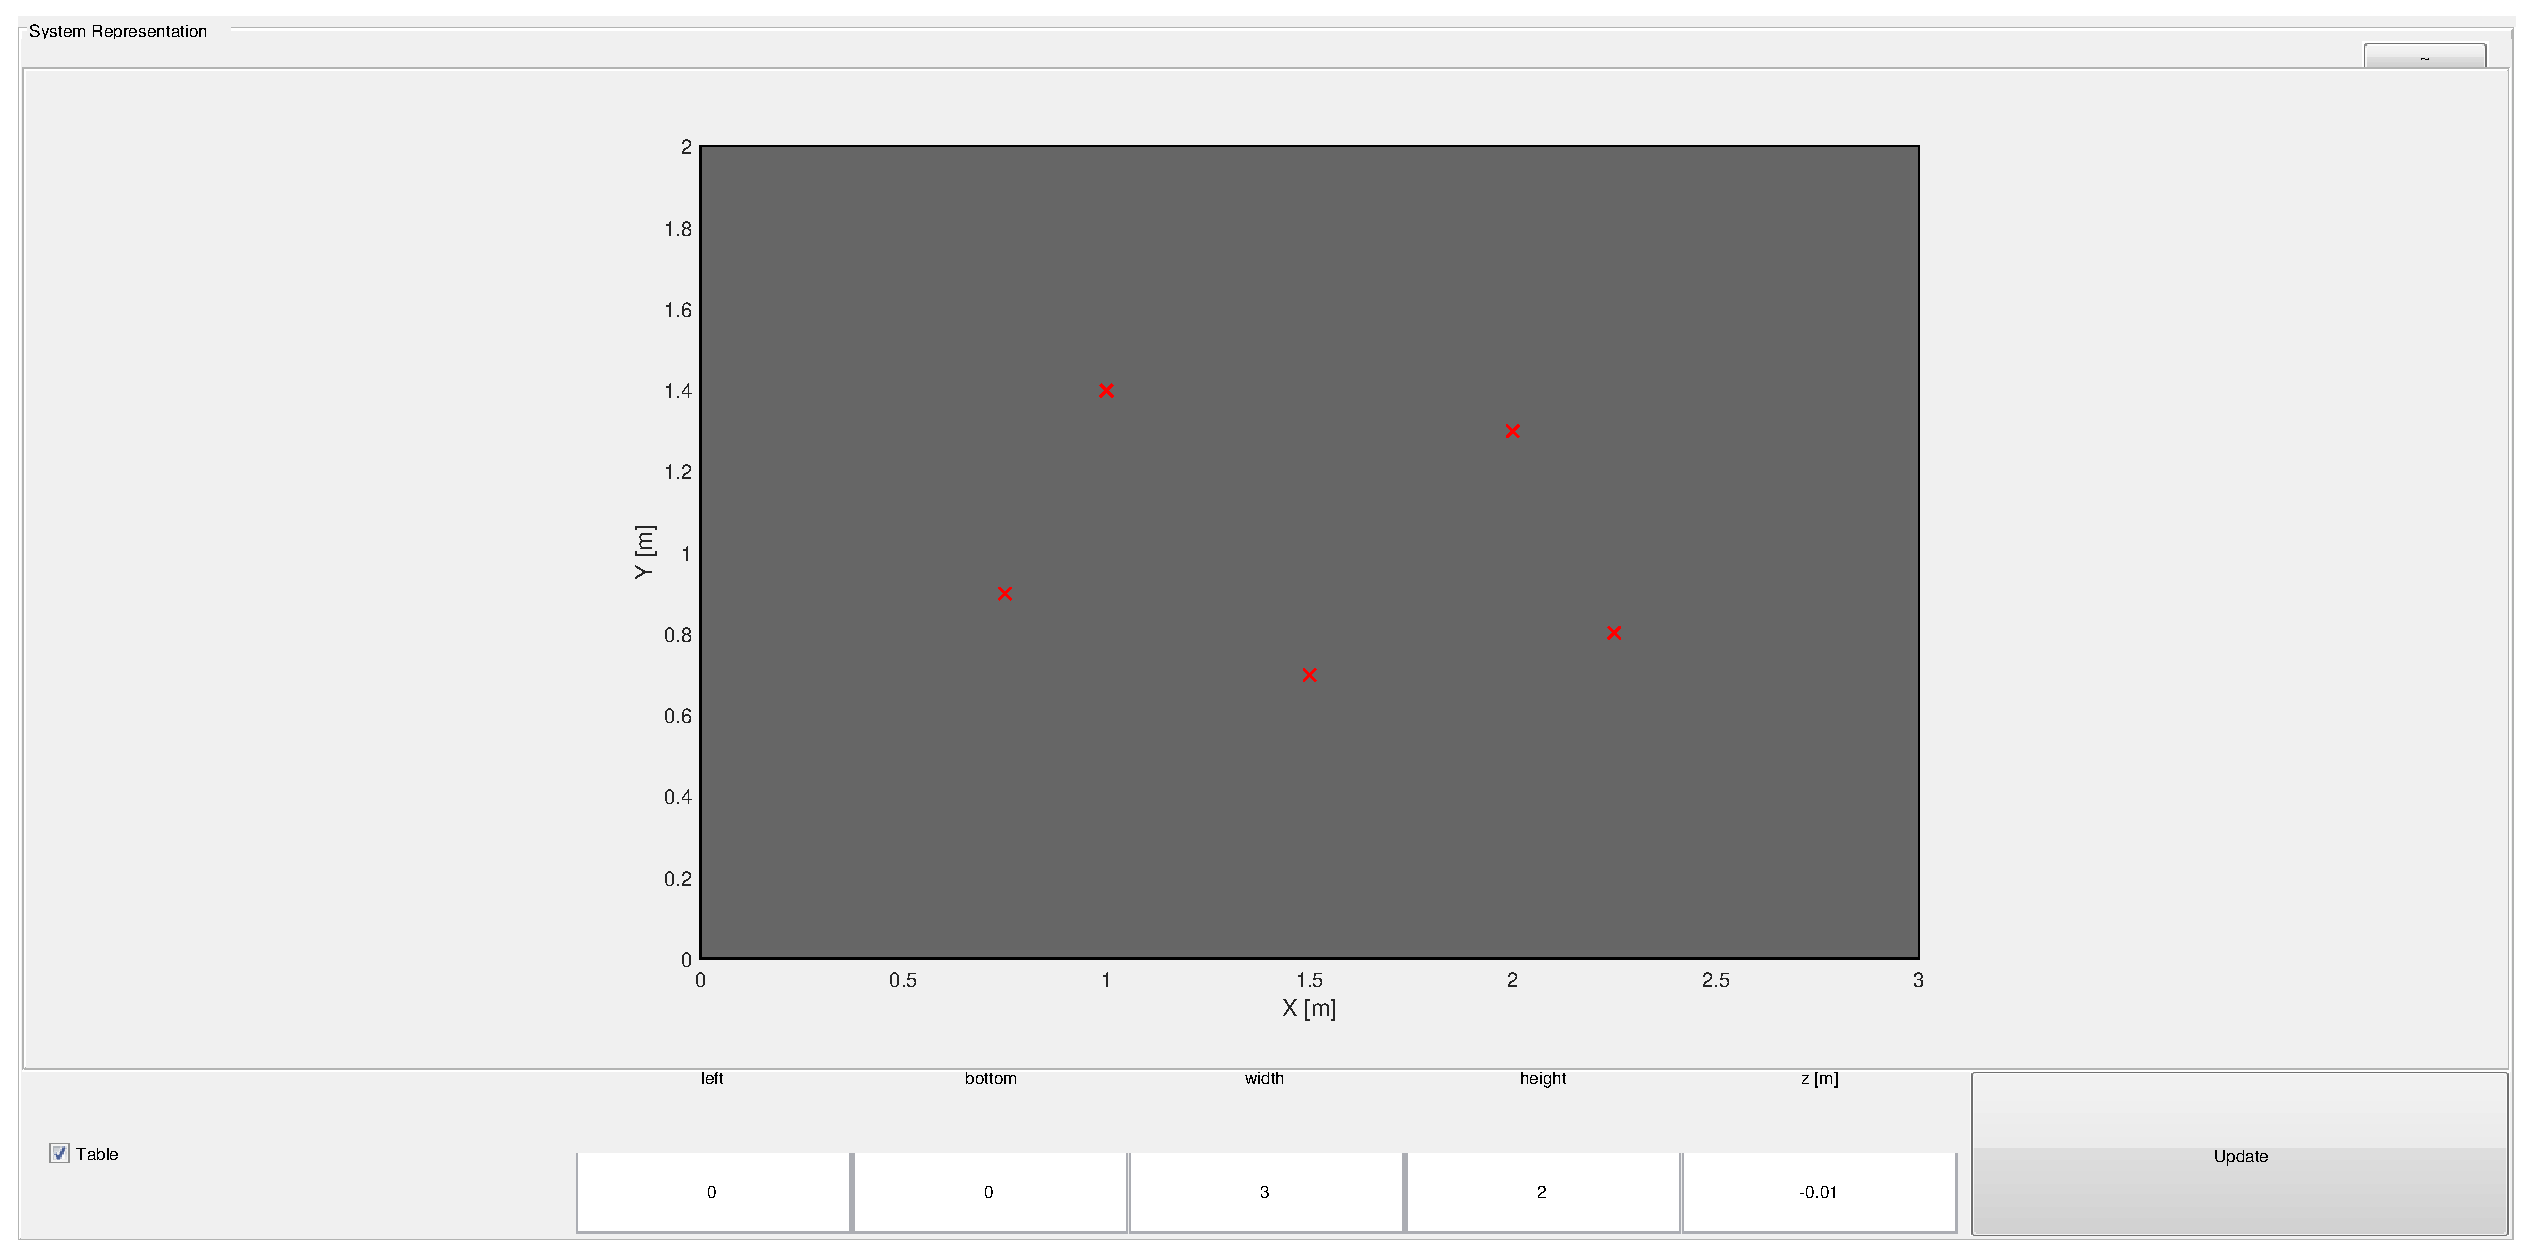
\includegraphics[width = \linewidth, clip=true, trim = 9.75cm 3.25cm 		9.0cm 1.1cm] {mic_array_example}} % l b r t]
%		\caption{EXAMPLE Microphone setup A} 
%		\label{fig:arrayA}
%	\endminipage \hfill
%	\minipage{0.32\textwidth}
%		\fbox{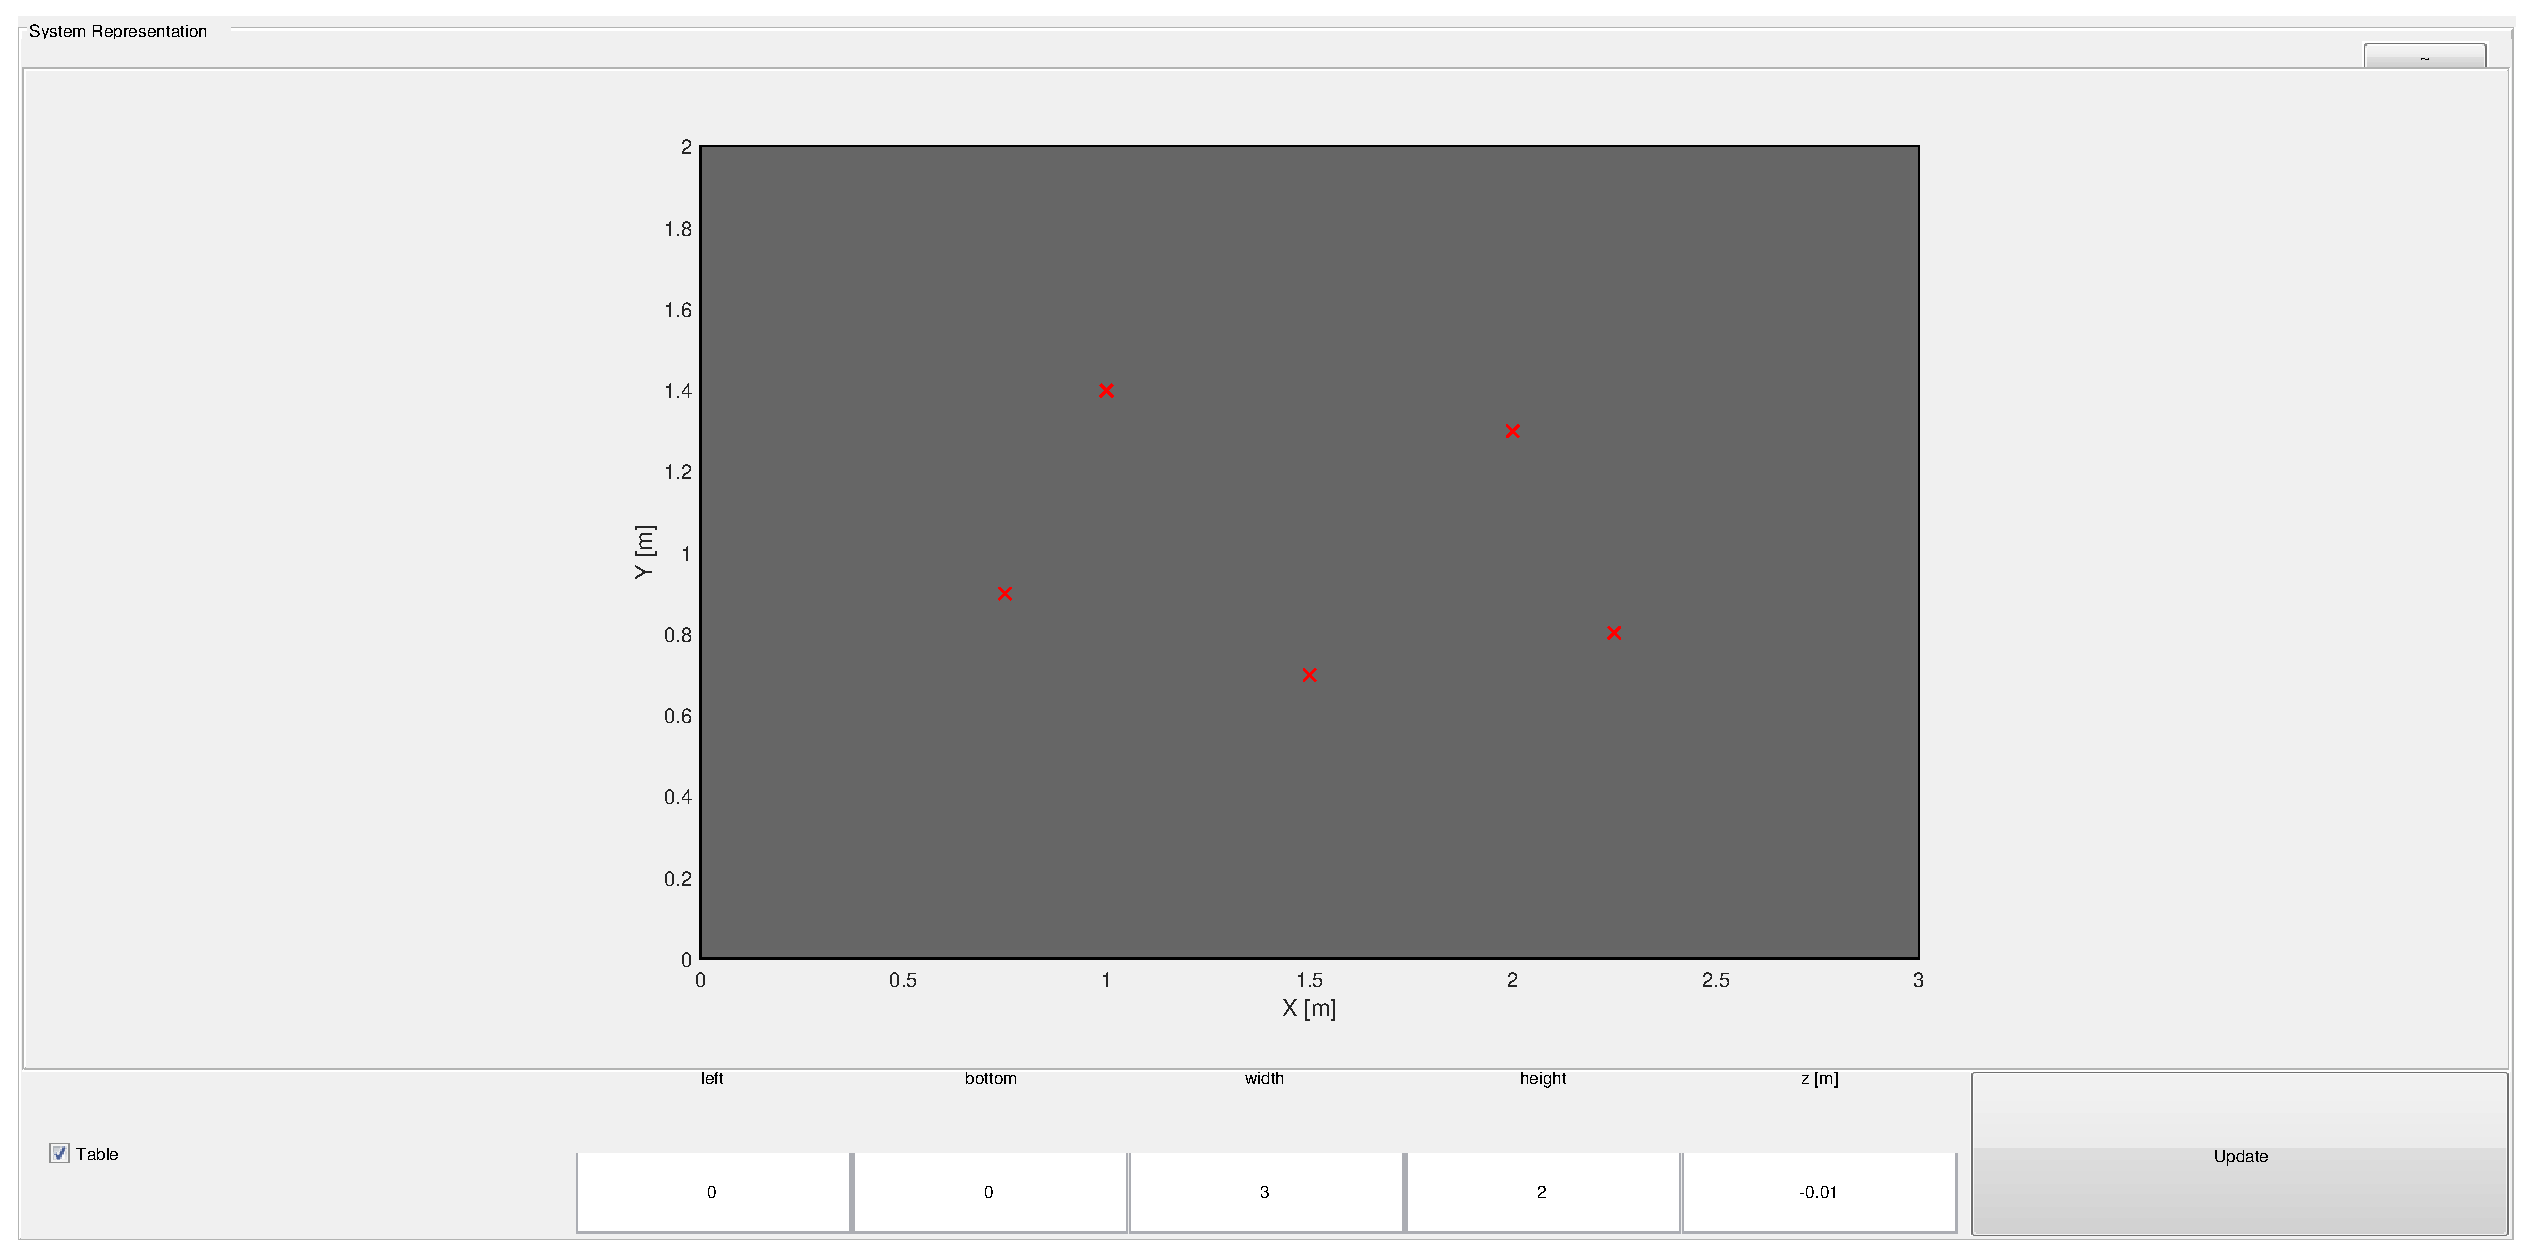
\includegraphics[width = \linewidth, clip=true, trim = 9.75cm 3.25cm 		9.0cm 1.1cm] {mic_array_example}} % l b r t]
%		\caption{EXAMPLE Microphone setup B} 
%		\label{fig:arrayB}
%	\endminipage \hfill
%	\minipage{0.32\textwidth}
%		\fbox{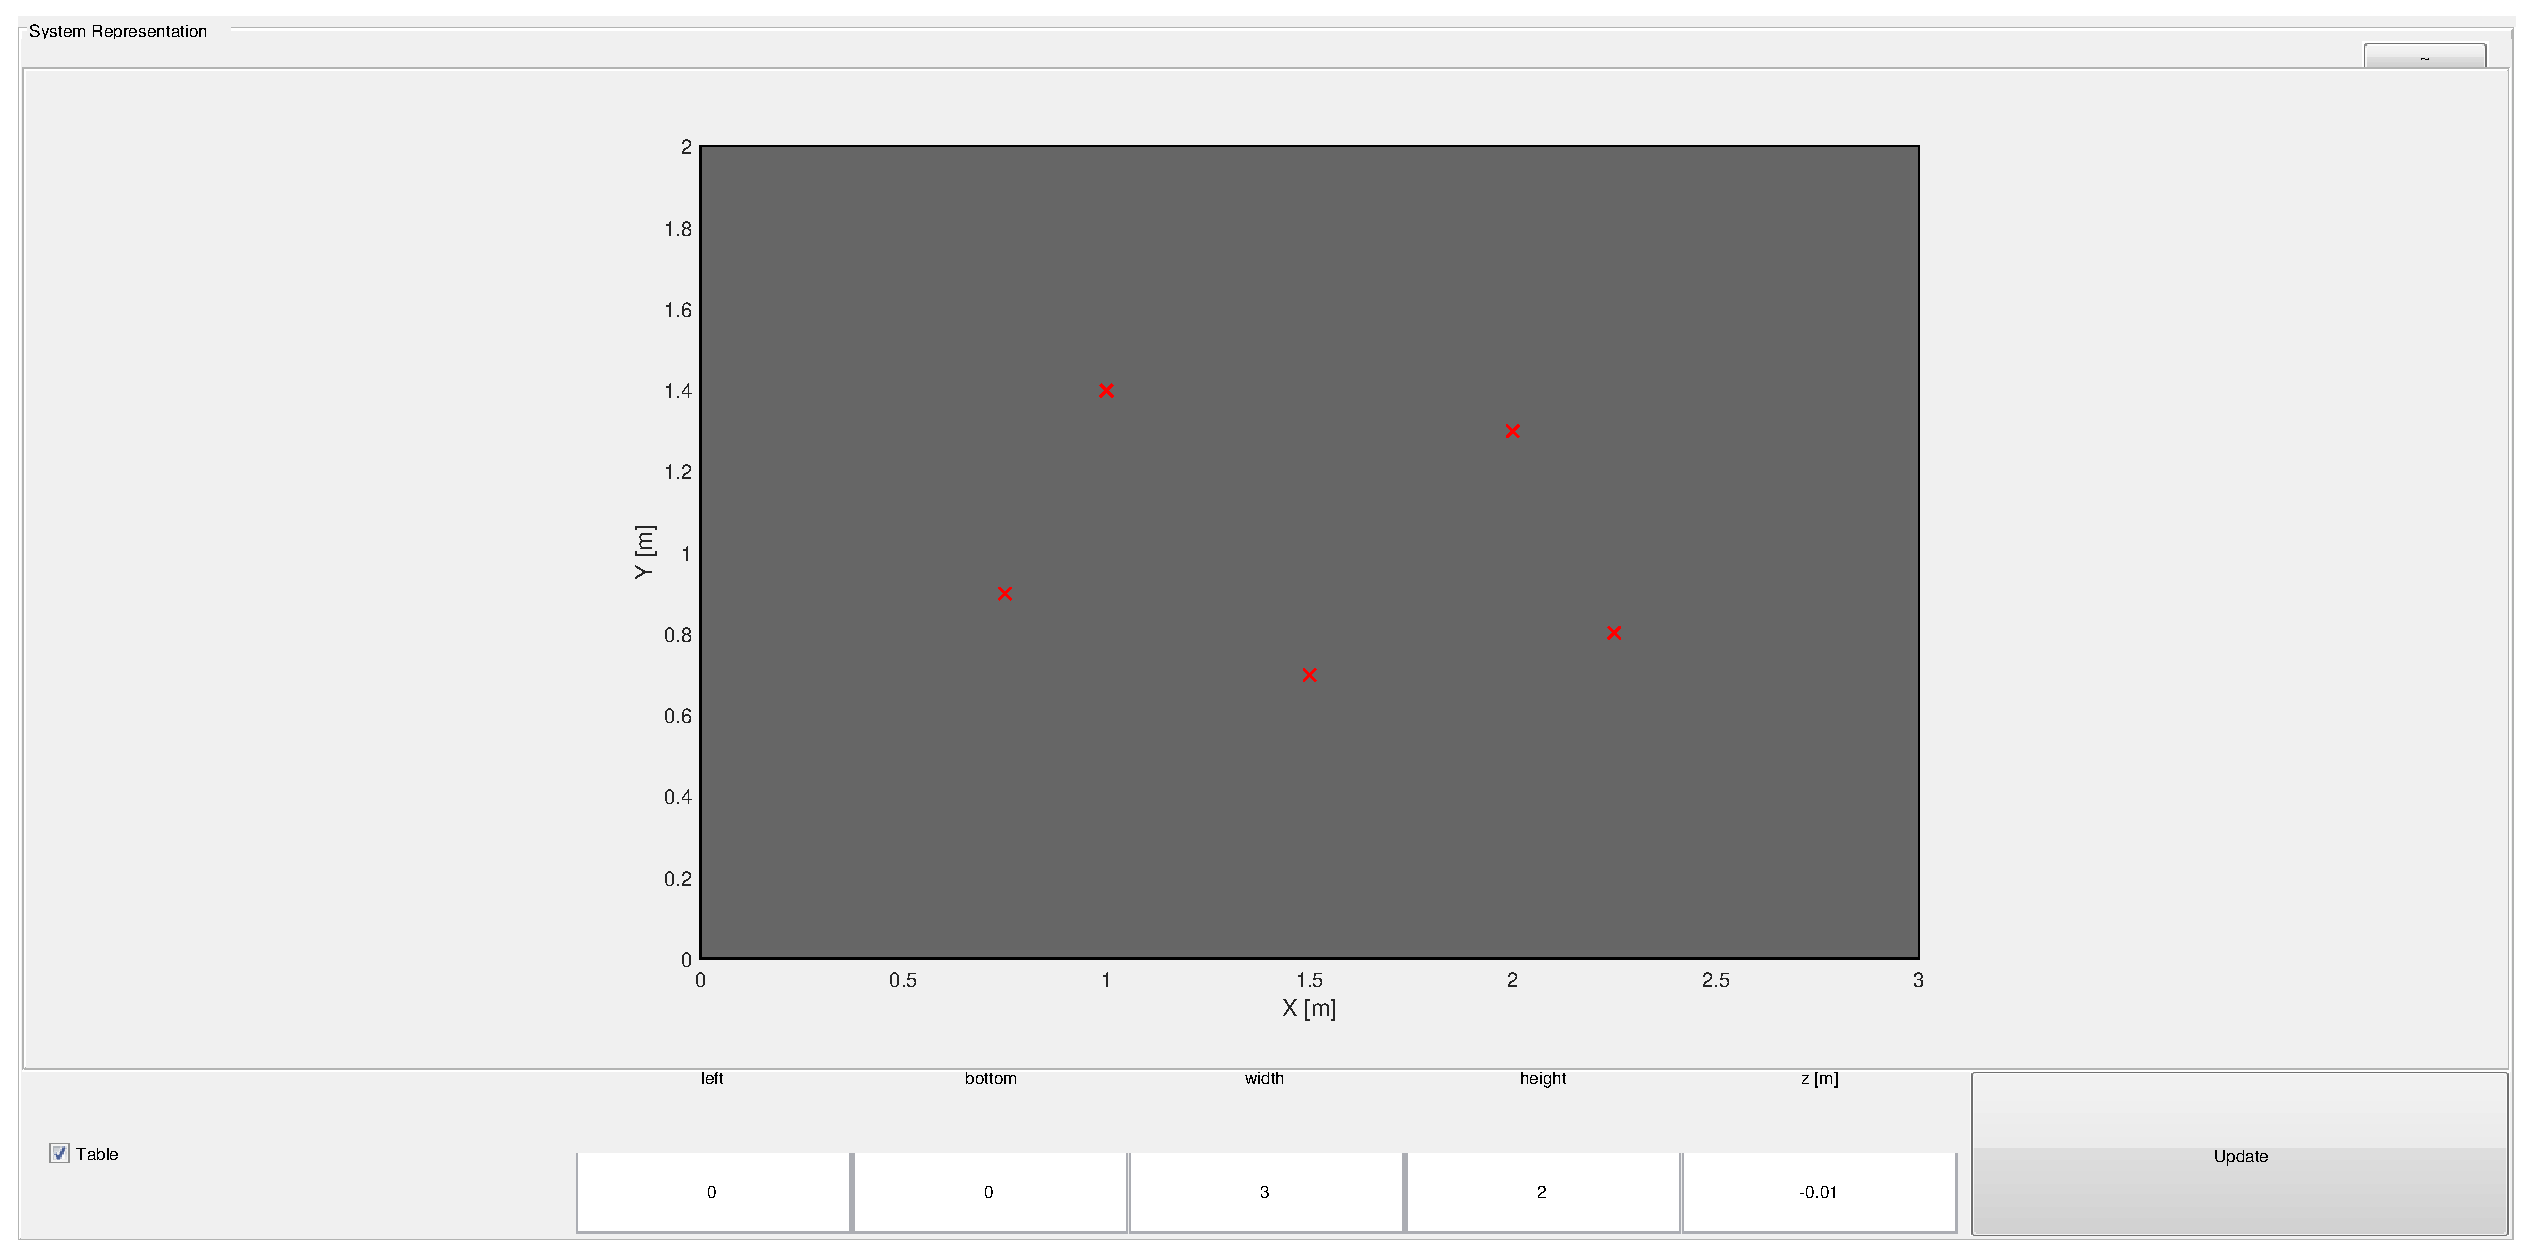
\includegraphics[width = \linewidth, clip=true, trim = 9.75cm 3.25cm 		9.0cm 1.1cm] {mic_array_example}} % l b r t]
%		\caption{EXAMPLE Microphone setup C} 
%		\label{fig:arrayC}
%	\endminipage%
%\end{figure}

%\begin{figure}
%\centering
%\begin{subfigure}{.5\textwidth}
%  \centering
%  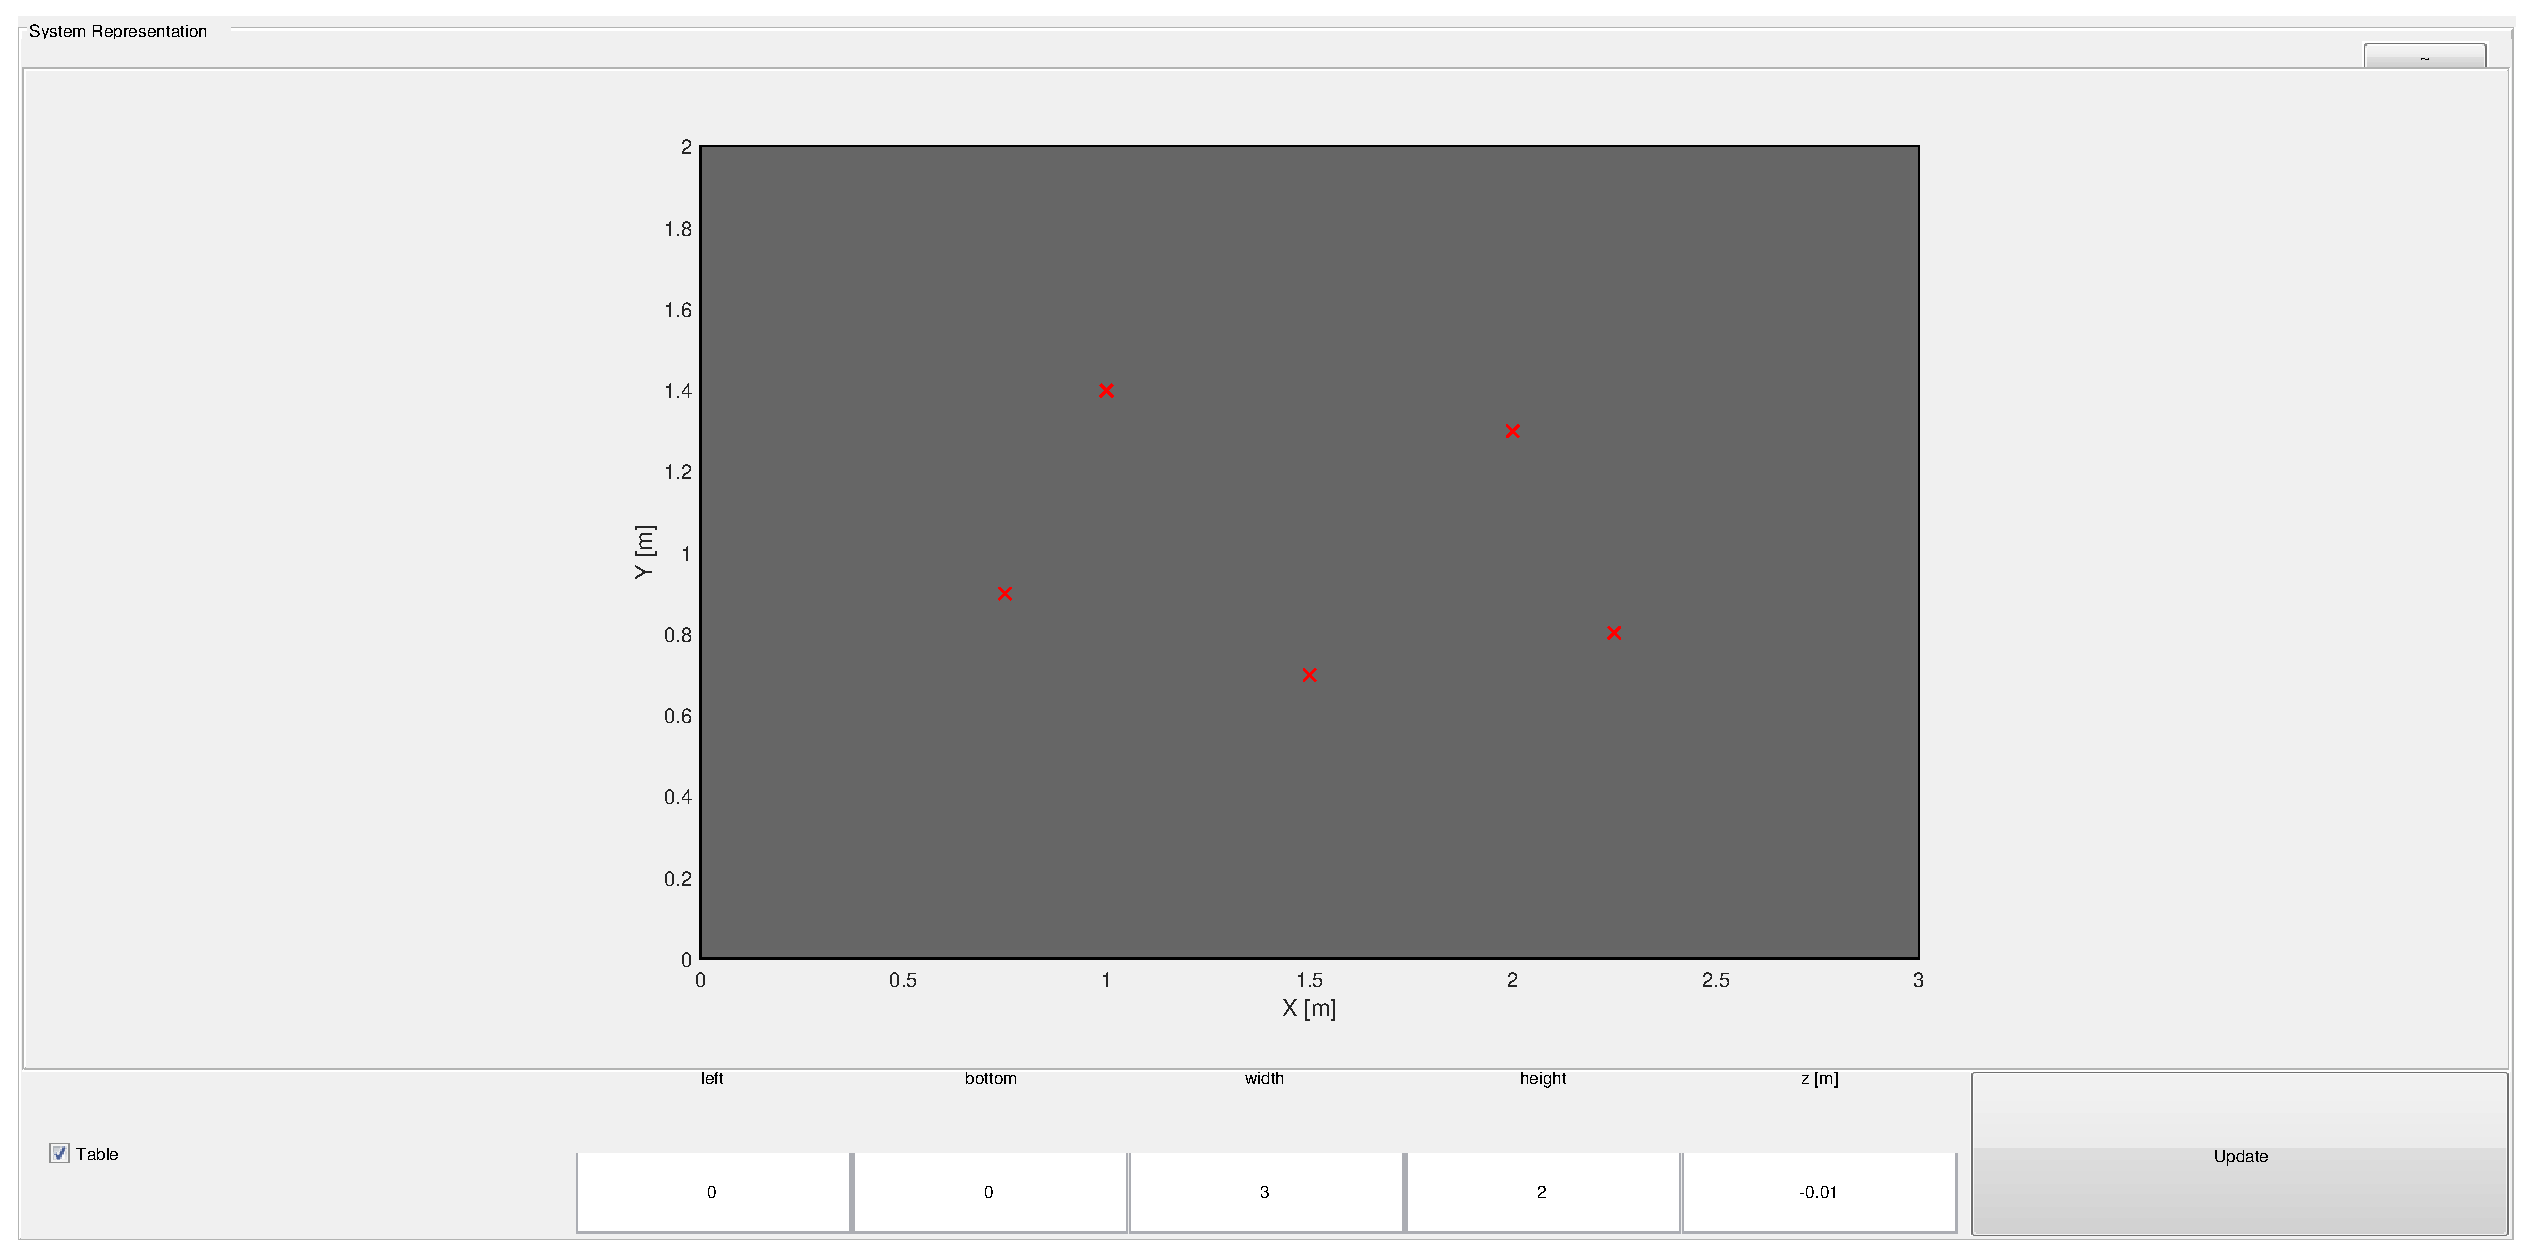
\includegraphics[width = \linewidth, clip=true, trim = 9.75cm 3.25cm 		9.0cm 1.1cm] {mic_array_example}
%  \caption{EXAMPLE Microphone setup A}
%  \label{fig:arrayA}
%\end{subfigure}%
%\begin{subfigure}{.5\textwidth}
%  \centering
%  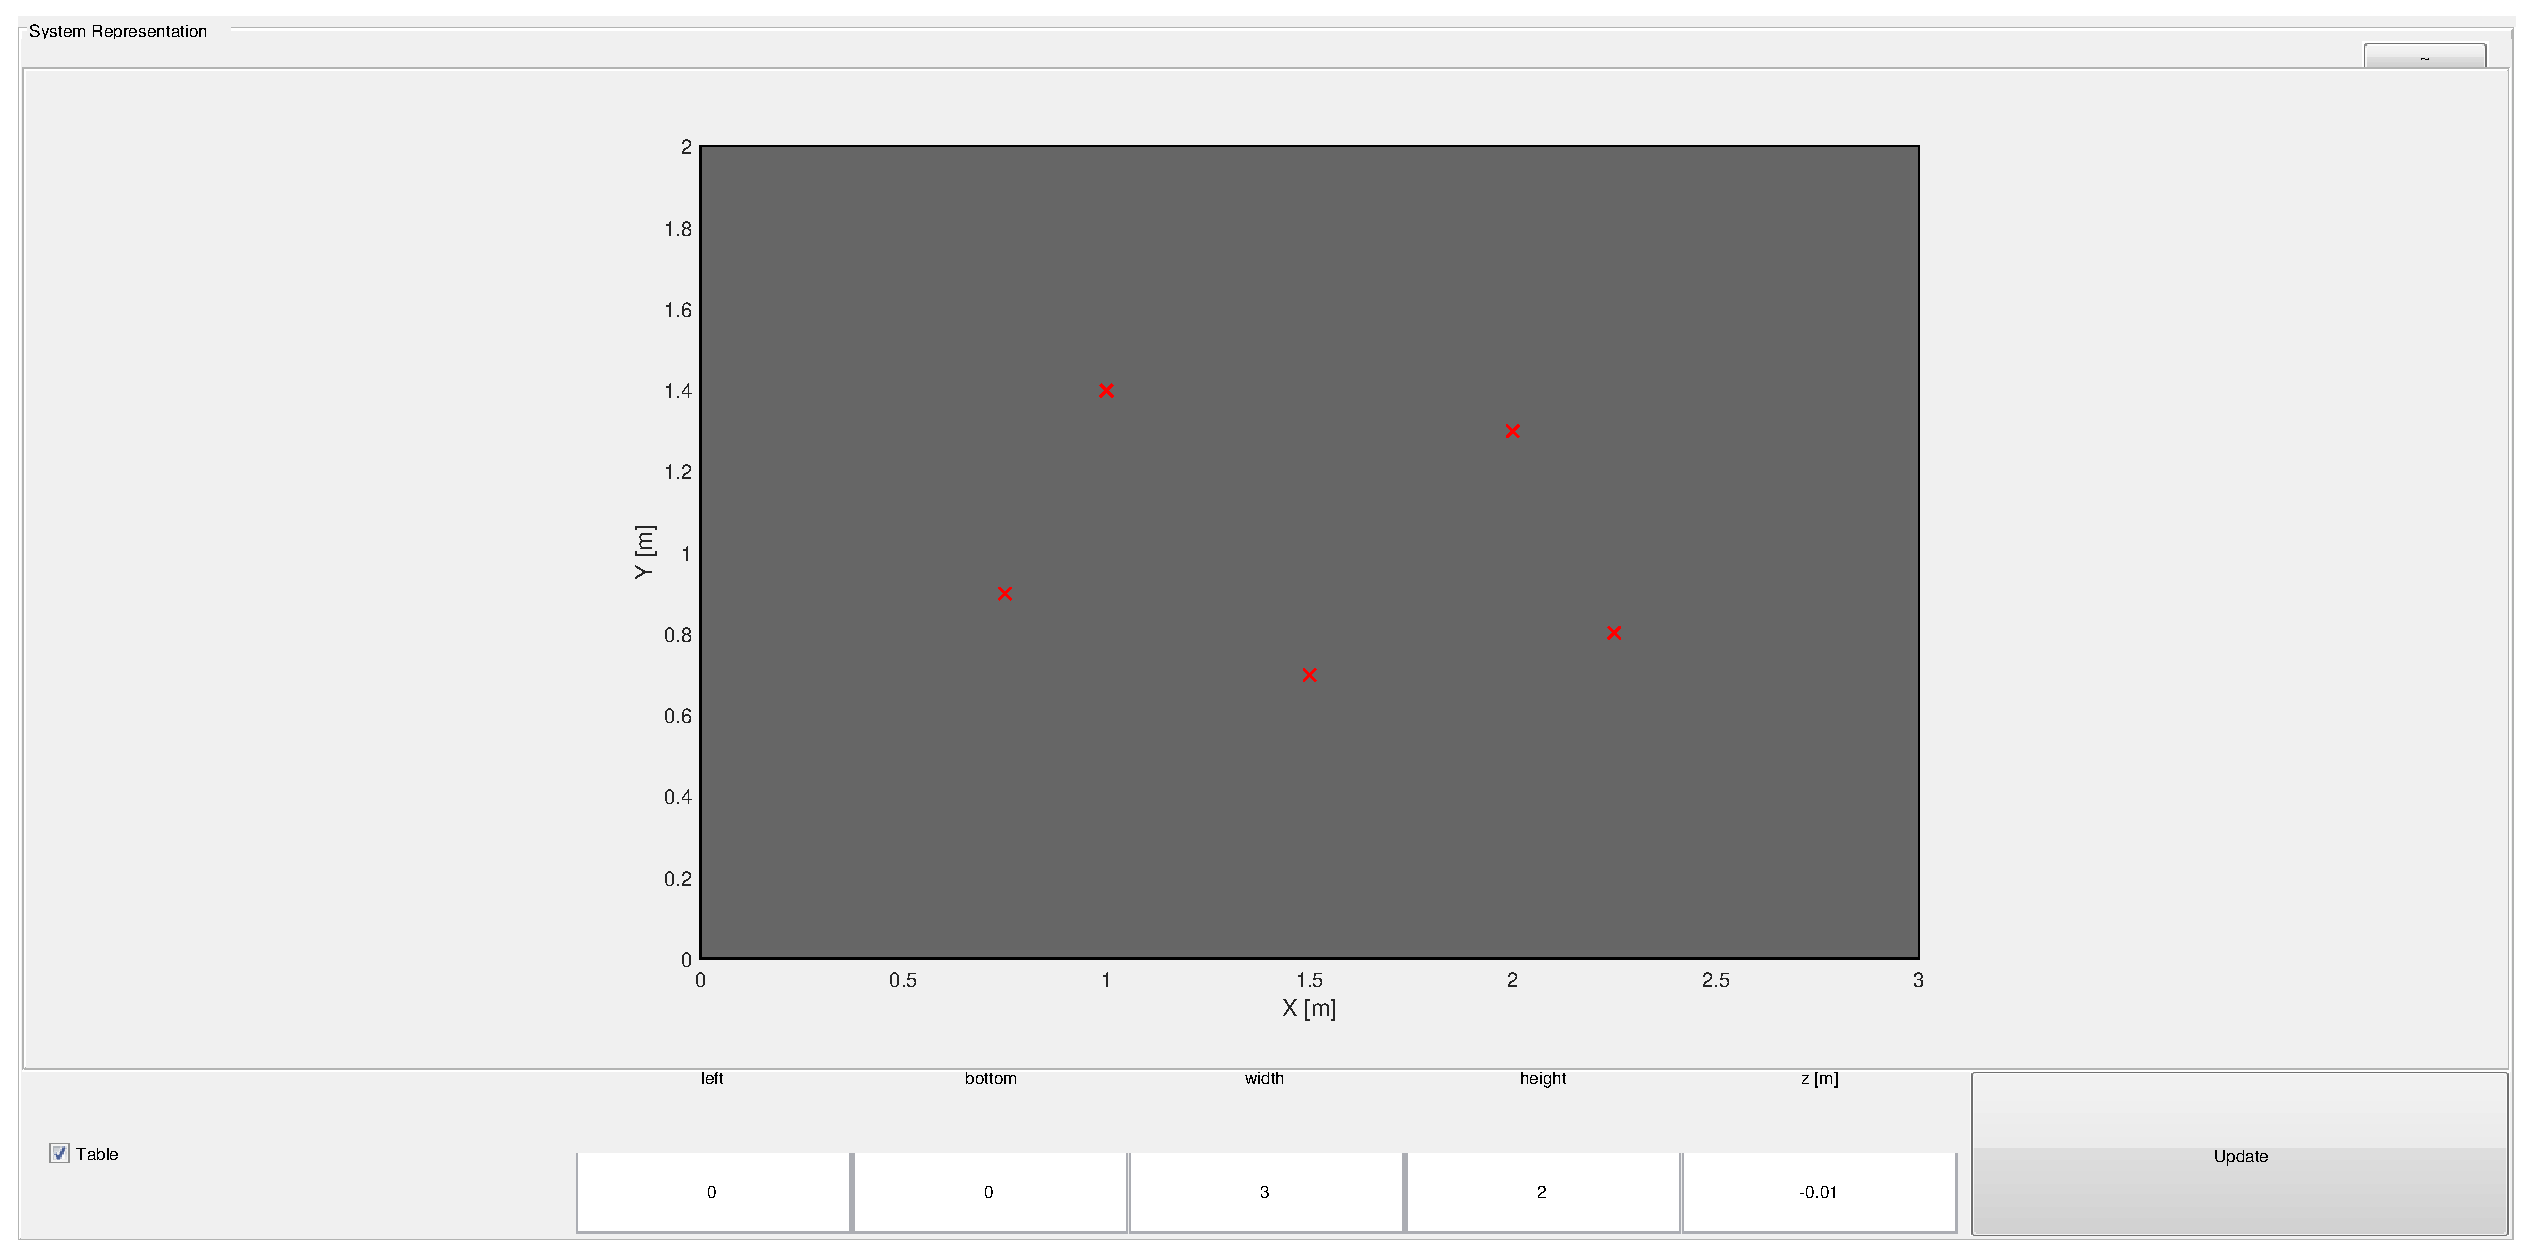
\includegraphics[width = \linewidth, clip=true, trim = 9.75cm 3.25cm 		9.0cm 1.1cm] {mic_array_example}
%  \caption{EXAMPLE Microphone setup B}
%  \label{fig:arrayB}
%\end{subfigure}
%\caption[Microphone setups used during the experiments] {A figure with two subfigures}
%\label{fig:test}
%\end{figure}



%\vspace{\baselineskip}
%{\Huge Possible tables:} \\
%\vspace{\baselineskip}
%\begin{tabular}{|c|c|c|c|c|c|c|}
%\hline 
%• & SNR & SNR seg & WNG & Array Gain & STOI & PESQ \\ 
%\hline 
%Closest Mic & • & • & • & • & • & • \\ 
%\hline 
%DSB & • & • & • & • & • & • \\ 
%\hline 
%MVDR & • & • & • & • & • & • \\ 
%\hline 
%MVDR+ & • & • & • & • & • & • \\ 
%\hline 
%\end{tabular}
%\vspace{\baselineskip}
%Or \\
%\vspace{\baselineskip}
%
%\textit{FOR EXAMPLE}
%The segmental SNR for the different microphone arrays:
%
%\begin{tabular}{|c|c|c|c|c|c|c|}
%\hline 
%Microphone array & Closest Mic & DSB & MVDR & MVDR+ \\ 
%\hline 
%A & • & • & • & • \\ 
%\hline 
%B & • & • & • & • \\ 
%\hline 
%C & • & • & • & • \\ 
%\hline 
%D & • & • & • & • \\ 
%\hline 
%\end{tabular}

%\vspace{\baselineskip}
%
%\begin{sidewaystable}[h]
%\centering
%
%\caption[Experimental results belonging to microphone array A]{Microphone array A}
%\label{tab:resultsA}
%  \begin{adjustbox}{max width=\textwidth}
%\begin{tabular}{|c|c|c|c|c|c|c|c|c|c|c|c|c|c|c|c|c|}
%\hline
%Beamformer 	& \multicolumn{4}{c|}{Simulation} 	& \multicolumn{4}{c|}{$\theta$ = theta1} & \multicolumn{4}{c|}{$\theta$ = theta2} & \multicolumn{4}{c|}{$\theta$ = theta3} \\ \hline
%Performance measure & SNR & $\text{SNR}_\text{seg}$ & STOI & PESQ &	& &	& &	& & & & & & & \\ \hline
%Closest 	& 	$SNR$ Simulation	& $SNR_{seg}$ Simulation& $STOI$ Simulation & $PESQ$ Simulation 	& $SNR$ theta1 & $SNR_{seg}$ theta1 & $STOI$ theta1 & $PESQ$ theta1								& 	$SNR$ theta2		& $SNR_{seg}$ theta2	& $STOI$ theta2 	& $PESQ$ theta2			& $SNR$ theta3 & $SNR_{seg}$ theta3	& $STOI$ theta3	& $PESQ$ theta3 \\
%DSB 		& 	$SNR$ Simulation	& $SNR_{seg}$ Simulation& $STOI$ Simulation & $PESQ$ Simulation 	& $SNR$ theta1 & $SNR_{seg}$ theta1 & $STOI$ theta1 & $PESQ$ theta1								& 	$SNR$ theta2		& $SNR_{seg}$ theta2	& $STOI$ theta2 	& $PESQ$ theta2			& $SNR$ theta3 & $SNR_{seg}$ theta3	& $STOI$ theta3	& $PESQ$ theta3 \\
%MVDR    	& 	$SNR$ Simulation	& $SNR_{seg}$ Simulation& $STOI$ Simulation & $PESQ$ Simulation 	& $SNR$ theta1 & $SNR_{seg}$ theta1 & $STOI$ theta1 & $PESQ$ theta1								& 	$SNR$ theta2		& $SNR_{seg}$ theta2	& $STOI$ theta2 	& $PESQ$ theta2			& $SNR$ theta3 & $SNR_{seg}$ theta3	& $STOI$ theta3	& $PESQ$ theta3 \\
%MVDR+  		& 	$SNR$ Simulation	& $SNR_{seg}$ Simulation& $STOI$ Simulation & $PESQ$ Simulation 	& $SNR$ theta1 & $SNR_{seg}$ theta1 & $STOI$ theta1 & $PESQ$ theta1								& 	$SNR$ theta2		& $SNR_{seg}$ theta2	& $STOI$ theta2 	& $PESQ$ theta2			& $SNR$ theta3 & $SNR_{seg}$ theta3	& $STOI$ theta3	& $PESQ$ theta3 \\ \hline
%\end{tabular}
%\end{adjustbox}
%
%\vspace{\baselineskip}
%
%\caption[Experimental results belonging to microphone array B]{Microphone array B}
%\label{tab:resultsB}
%  \begin{adjustbox}{max width=\textwidth}
%\begin{tabular}{|l|l|l|l|l|l|l|l|l|l|l|l|l|l|l|l|l|}
%\hline
%Beamformer 	& \multicolumn{4}{c|}{Simulation} 	& \multicolumn{4}{c|}{$\theta$ = theta1} & \multicolumn{4}{c|}{$\theta$ = theta2} & \multicolumn{4}{c|}{$\theta$ = theta3} \\ \hline
% & & & & &	& &	& &	& & & & & & & \\
%Closest 	& 	$SNR$ Simulation	& $SNR_{seg}$ Simulation& $STOI$ Simulation & $PESQ$ Simulation 	& $SNR$ theta1 & $SNR_{seg}$ theta1 & $STOI$ theta1 & $PESQ$ theta1								& 	$SNR$ theta2		& $SNR_{seg}$ theta2	& $STOI$ theta2 	& $PESQ$ theta2			& $SNR$ theta3 & $SNR_{seg}$ theta3	& $STOI$ theta3	& $PESQ$ theta3 \\
%DSB 		& 	$SNR$ Simulation	& $SNR_{seg}$ Simulation& $STOI$ Simulation & $PESQ$ Simulation 	& $SNR$ theta1 & $SNR_{seg}$ theta1 & $STOI$ theta1 & $PESQ$ theta1								& 	$SNR$ theta2		& $SNR_{seg}$ theta2	& $STOI$ theta2 	& $PESQ$ theta2			& $SNR$ theta3 & $SNR_{seg}$ theta3	& $STOI$ theta3	& $PESQ$ theta3 \\
%MVDR    	& 	$SNR$ Simulation	& $SNR_{seg}$ Simulation& $STOI$ Simulation & $PESQ$ Simulation 	& $SNR$ theta1 & $SNR_{seg}$ theta1 & $STOI$ theta1 & $PESQ$ theta1								& 	$SNR$ theta2		& $SNR_{seg}$ theta2	& $STOI$ theta2 	& $PESQ$ theta2			& $SNR$ theta3 & $SNR_{seg}$ theta3	& $STOI$ theta3	& $PESQ$ theta3 \\
%MVDR+  		& 	$SNR$ Simulation	& $SNR_{seg}$ Simulation& $STOI$ Simulation & $PESQ$ Simulation 	& $SNR$ theta1 & $SNR_{seg}$ theta1 & $STOI$ theta1 & $PESQ$ theta1								& 	$SNR$ theta2		& $SNR_{seg}$ theta2	& $STOI$ theta2 	& $PESQ$ theta2			& $SNR$ theta3 & $SNR_{seg}$ theta3	& $STOI$ theta3	& $PESQ$ theta3 \\ \hline
%\end{tabular}
%\end{adjustbox}
%
%\vspace{\baselineskip}
%
%\caption[Experimental results belonging to microphone array C]{Microphone array C}
%\label{tab:resultsC}
%  \begin{adjustbox}{max width=\textwidth}
%\begin{tabular}{|l|l|l|l|l|l|l|l|l|l|l|l|l|l|l|l|l|}
%\hline
%Beamformer 	& \multicolumn{4}{c|}{Simulation} 	& \multicolumn{4}{c|}{$\theta$ = theta1} & \multicolumn{4}{c|}{$\theta$ = theta2} & \multicolumn{4}{c|}{$\theta$ = theta3} \\ \hline
% & & & & &	& &	& &	& & & & & & & \\
%Closest 	& 	$SNR$ Simulation	& $SNR_{seg}$ Simulation& $STOI$ Simulation & $PESQ$ Simulation 	& $SNR$ theta1 & $SNR_{seg}$ theta1 & $STOI$ theta1 & $PESQ$ theta1								& 	$SNR$ theta2		& $SNR_{seg}$ theta2	& $STOI$ theta2 	& $PESQ$ theta2			& $SNR$ theta3 & $SNR_{seg}$ theta3	& $STOI$ theta3	& $PESQ$ theta3 \\
%DSB 		& 	$SNR$ Simulation	& $SNR_{seg}$ Simulation& $STOI$ Simulation & $PESQ$ Simulation 	& $SNR$ theta1 & $SNR_{seg}$ theta1 & $STOI$ theta1 & $PESQ$ theta1								& 	$SNR$ theta2		& $SNR_{seg}$ theta2	& $STOI$ theta2 	& $PESQ$ theta2			& $SNR$ theta3 & $SNR_{seg}$ theta3	& $STOI$ theta3	& $PESQ$ theta3 \\
%MVDR    	& 	$SNR$ Simulation	& $SNR_{seg}$ Simulation& $STOI$ Simulation & $PESQ$ Simulation 	& $SNR$ theta1 & $SNR_{seg}$ theta1 & $STOI$ theta1 & $PESQ$ theta1								& 	$SNR$ theta2		& $SNR_{seg}$ theta2	& $STOI$ theta2 	& $PESQ$ theta2			& $SNR$ theta3 & $SNR_{seg}$ theta3	& $STOI$ theta3	& $PESQ$ theta3 \\
%MVDR+  		& 	$SNR$ Simulation	& $SNR_{seg}$ Simulation& $STOI$ Simulation & $PESQ$ Simulation 	& $SNR$ theta1 & $SNR_{seg}$ theta1 & $STOI$ theta1 & $PESQ$ theta1								& 	$SNR$ theta2		& $SNR_{seg}$ theta2	& $STOI$ theta2 	& $PESQ$ theta2			& $SNR$ theta3 & $SNR_{seg}$ theta3	& $STOI$ theta3	& $PESQ$ theta3 \\ \hline
%\end{tabular}
%\end{adjustbox}
%\end{sidewaystable}

%\begin{sidewaystable}[h]
%\centering
%
%\caption[]{Experimental results including interference}
%\label{tab:resultsA}
%  \begin{adjustbox}{max width=\textwidth}
%\begin{tabular}{|c|c|c|c|c|c|c|c|c|c|c|c|c|c|c|c|c|}
%\hline
%• & \multicolumn{4}{c|}{Simulation}	& \multicolumn{4}{c|}{$\theta$ = theta1} & \multicolumn{4}{c|}{$\theta$ = theta2}  \\ \hline
%
%Beamformer				& Closest  	& DSB 	& MVDR 	& MVDR+ & Closest  	& DSB 	& MVDR 	& MVDR+ & Closest  	& DSB 	& MVDR 	& MVDR+ \\ \hline
%
%Performance measure 	& •	& •& • & • & • & • & • & • & • & • & • & •  \\
%
%$SNR$ 					& •	& •& • & • & -6.8 & -5.8 & -7.0 & -29.9 & -7.3 & -6.3 & -8.9 & -31.2  \\
%
%$SNR_{seg}$ 			& •	& •& • & • & -6.7 & -5.0 & -7.8 & -32.5 & -7.8 & -6.1 & -9.7 & -33.8 \\
%
%$STOI$    				& •	& •& • & • & 0.70 & 0.79 & 0.64 & 0.65 & 0.66 & 0.72 & 0.56 & 0.58 \\
%
%$PESQ$  				& •	& •& • & • & 2.32 & 2.54 & 1.81 & 1.89 & 2.10 & 2.37 & 1.72 & 1.83 \\
%
%$Array gain$  			& •	& •& • & • &      & 0.86 & 1.03 & 4.39 & 	  & 0.86 & 1.22 & 4.25 \\
%
%$White noise gain$ 		& •	& •& • & • &  	  & -4.64 & 52.82 & 105.08 &   & -4.64 & 52.33 & 96.53 \\ \hline
%
%• & \multicolumn{4}{c|}{$\theta$ = theta3} & \multicolumn{4}{c|}{$\theta$ = theta4} & \multicolumn{4}{c|}{Linear array} \\ \hline
%
%Beamformer				& Closest  	& DSB 	& MVDR 	& MVDR+ & Closest  	& DSB 	& MVDR 	& MVDR+ & Closest  	& DSB 	& MVDR 	& MVDR+ \\ \hline
%
%Performance measure 	& •	& •& • & • & • & • & • & • & • & • & • & •  \\
%
%$SNR$ 					& -6.7	& -6.5	& -13.8 & -53 	& -6.8	& -6.0 & -7.9 & -28.5 & -7.1	& -6.2& -7.2 & -34.1   \\
%
%$SNR_{seg}$ 			& -7.3	& -7.6	& -15.7 & -55.6 & -7.5	& -5.9 & -8.8 & -31.1 & -7.6	& -6.2& -8.1 & -36.7   \\
%
%$STOI$    				& 0.65	& 0.65	& 0.48 & 0.47 	& 0.64	& 0.73 & 0.58 & 0.60 & 0.67		& 0.70& 0.53 & 0.54   \\
%
%$PESQ$  				& 2.06	& 1.97	& 1.29 & 1.39 	& 2.08	& 2.36 & 1.72 & 1.81 & 2.12 	& 2.30& 1.68 & 1.80   \\
%
%$Array gain$  			&  		& 0.96 	& 2.05 & 7.86 	& 		& 0.88	& 1.16 & 4.20 &  		& 0.86& 1.01 & 4.78   \\
%
%$White noise gain$ 		&  		& -4.64	& 51.96 & 93.82 & 		& -4.64 & 52.24 & 98.88 &  		& -4.77 & 54.56 & 104.99   \\
%
%
%\end{tabular}
%\end{adjustbox}
%\end{sidewaystable}






%\hline \hline 
%\multicolumn{13}{|c|}{\multirow{2}{*}{With an interfering audio source}} \\ 
%\multicolumn{13}{|l|}{} \\ \hline
%
%• & \multicolumn{4}{c|}{Simulation}	& \multicolumn{4}{c|}{$\theta$ = theta1} & \multicolumn{4}{c|}{$\theta$ = theta2}  \\ \hline
%
%Beamformer				& Closest  	& DSB 	& MVDR 	& MVDR+ & Closest  	& DSB 	& MVDR 	& MVDR+ & Closest  	& DSB 	& MVDR 	& MVDR+ \\ \hline
%
%Performance measure 	& •	& •& • & • & • & • & • & • & • & • & • & •  \\
%
%$SNR$ 					& •	& •& • & • & -6.8 & -5.8 & -7.0 & -29.9 & -7.3 & -6.3 & -8.9 & -31.2  \\
%
%$SNR_{seg}$ 			& •	& •& • & • & -6.7 & -5.0 & -7.8 & -32.5 & -7.8 & -6.1 & -9.7 & -33.8 \\
%
%$STOI$    				& •	& •& • & • & 0.70 & 0.79 & 0.64 & 0.65 & 0.66 & 0.72 & 0.56 & 0.58 \\
%
%$PESQ$  				& •	& •& • & • & 2.32 & 2.54 & 1.81 & 1.89 & 2.10 & 2.37 & 1.72 & 1.83 \\
%
%$Array gain$  			& •	& •& • & • &      & 0.86 & 1.03 & 4.39 & 	  & 0.86 & 1.22 & 4.25 \\
%
%$White noise gain$ 		& •	& •& • & • &  	  & -4.64 & 52.82 & 105.08 &   & -4.64 & 52.33 & 96.53 \\ \hline
%
%• & \multicolumn{4}{c|}{$\theta$ = theta3} & \multicolumn{4}{c|}{$\theta$ = theta4} & \multicolumn{4}{c|}{Linear array} \\ \hline
%
%Beamformer				& Closest  	& DSB 	& MVDR 	& MVDR+ & Closest  	& DSB 	& MVDR 	& MVDR+ & Closest  	& DSB 	& MVDR 	& MVDR+ \\ \hline
%
%Performance measure 	& •	& •& • & • & • & • & • & • & • & • & • & •  \\
%
%$SNR$ 					& -6.7	& -6.5	& -13.8 & -53 	& -6.8	& -6.0 & -7.9 & -28.5 & -7.1	& -6.2& -7.2 & -34.1   \\
%
%$SNR_{seg}$ 			& -7.3	& -7.6	& -15.7 & -55.6 & -7.5	& -5.9 & -8.8 & -31.1 & -7.6	& -6.2& -8.1 & -36.7   \\
%
%$STOI$    				& 0.65	& 0.65	& 0.48 & 0.47 	& 0.64	& 0.73 & 0.58 & 0.60 & 0.67		& 0.70& 0.53 & 0.54   \\
%
%$PESQ$  				& 2.06	& 1.97	& 1.29 & 1.39 	& 2.08	& 2.36 & 1.72 & 1.81 & 2.12 	& 2.30& 1.68 & 1.80   \\
%
%$Array gain$  			&  		& 0.96 	& 2.05 & 7.86 	& 		& 0.88	& 1.16 & 4.20 &  		& 0.86& 1.01 & 4.78   \\
%
%$White noise gain$ 	&  		& -4.64	& 51.96 & 93.82 & 		& -4.64 & 52.24 & 98.88 &  		& -4.77 & 54.56 & 104.99   \\
\chapter{Discussion}
\label{chap:discussion}
%Vergelijking met related research en onze resultaten, specifiek overeenkomsten en verschillen

Different experiments and simulations have been done to investigate the performance of the beamforming algorithms. The DSB is a simple beamforming algorithm compared to the MVDR beamforming algorithm and as discussed in section \ref{chap:related}, the DSB algorithm is optimal for spatially white noise. The delay-and-sum beamforming algorithm can be used as comparison for the other two beamforming algorithms. The MVDR algorithm was expected to perform well in the presence of coherent noise. Therefore it was expected that the MVDR algorithm would be the best performing beamformer in an office room scenario.

\section{Performance of the Beamforming Algorithms}
The simulated scenarios confirm the expectation that the MVDR beamforming algorithm has the best performance, but the conducted experiments lead to unexpected results. The DSB algorithm slightly enhanced the quality of the audio in the simulated scenarios and in the office room experiments but the MVDR only improved the sound quality in the simulated scenarios and in the anechoic scenario. A possible explanation for this could be the high white noise gain of the MVDR beamforming algorithm. In all the simulations and all the conducted measurements, the white noise gain for the MVDR beamformer was above $50dB$. A high white noise gain causes the beamforming algorithm to have a poor $SNR$ due to white noise contributions as explained in chapter \ref{chap:related}. The MVDR has a tendency to converge to the DSB when the white noise level is high \cite{gannot2010}.
Another reason could be the sensitivity of the MVDR to position errors. As proven in the simulations, the MVDR is highly sensitive to position errors. Inaccurately measured locations during the office room experiments could reduce the performance of the MVDR beamformer. Also inacuracy in speed of sound could be a factor in the performance decrease. The speed of sound varies with temperature and humidity, and this variation was not considered in the measurements.

%The segmental SNR was in all of the simulated scenarios lower than the global SNR...

%It is expected that an improvement in SNR results in an improvement in MOS and in our results...






\section{Possible improvements}
Localization and distributed calculation of the beamforming algorithms are not in the scope of this thesis, but are still closely related topics. The source and microphone locations are essential for the performance of a beamforming algorithm. In this research, there is still a central computer needed to run the beamforming algorithm. Hence it would be an improvement if the calculations of the beamforming algorithm could be done distributed on the smartphones. These distributed calculations could make a central processing unit redundant.

\subsection{Localization}

Brandstein et al. \cite{brandstein2001} divide source localization in three different classes, steered beamformer based locators, high resolution spectral estimation locators and time difference of arrival (TDOA) locators. Steered beamformer based locators scan the region to find the region which produces the highest output energy. High-resolution spectral estimation locators use a spectral phase correlation matrix to find the best fit for source localization. TDOA locators use the delay of the sound between microphones to calculate the location of the source. 

The locations of the microphones are, besides the location of the source, also of importance to the performance of the beamformer. A possible solution for this problem is the use of self-localization with high accuracy to find out the locations of the microphones \cite{hennecke2011}.

\subsection{Distributed algorithm}

A distributed algorithm for the DSB for wireless acoustic sensor networks, is proposed by Zeng et al. \cite{zeng2013, zeng2014}. A distributed MVDR beamformer for wireless acoustic sensor networks based on message passing is proposed in \cite{heusdens2012}.

\subsection{Realtime Beamforming Toolbox}
The \matlab toolbox developed for this project was very powerful in conducting the experiments and analyzing the data. The complete process has been automated. Future work on audio enhancement using smartphones could use this toolbox to record audio synchronously on smartphones.\\
Also the opportunity to add more different beamforming algorithms can be explored. There is an example processing class in which they can be included quite easily.








%\section{Remarks (from literature study)}
%The localization of the source is critical for the operation of a beamforming algorithm. Cha Zhang et al. \cite{zhang2008} propose an eMVDR which has good localization in reverberant environments. Instead of improving the localization, one can also make the algorithm less sensitive to a change of the source location \cite{ehrenberg2010}. Localization is generally performed by using time differences of arrival from one source to the multiple microphones. For this calculation, the locations of the microphones are assumed to be known. However, there is also the possibility to use self-localization to find out the locations of the microphones \cite{hennecke2011}.
%
%Differences in sample rate and time references between devices can heavily impact the effectiveness of the beamformer \cite{schm2013}. Possible solutions to this have been outlined in subsection 
%{\Huge ref!} %\ref{subsec:synch}}. 
%In addition, room reverberations can be very hard to invert because the ATF changes with time and with the position of the source \cite{jin2010}.
%
%Different kinds of noise call for different beamforming algorithms. The DSB has the property that it suppresses white noise sources well \cite{brandstein2001}, whereas the MVDR beamformer can suppress coherent noise sources \cite{naylor2010speech} better.
\chapter{Conclusion}
\label{chap:conclusion}

The goal of the research was to compare the performance of existing wide-band near-field beamforming algorithms in enhancing audio from microphone arrays, and the adaptation of directivity patterns in the microphone response. Measurements have been performed both in an anechoic environment and in a typical office environment. Data has been gathered and processed using the beamforming toolbox written for this project. The data was analyzed and compared in both objective and subjective metrics, as is common in the literature about this subject \citep{brandstein2001,gaubitch2014,martinez2015,griffiths1982,kjellson2014sound,ba2007,habets2010,doclo2003}. The objective audio quality measures show very high correlation with each other. They also show high correlation to the power ralated metrics, except when they are used on a very noisy signal. In that case both STOI and PESQ become unreliable.

\section{Simulation}
\label{sec:conc:sim}
The simulations show improvement on all metrics for both DSB and MVDR in the measurement scenario. They also show better intelligibility for MVDR than for DSB in all scenarios, for both STOI and PESQ.\newline
%\subsection{Power metrics}
%\label{sec:conc:sim:snr}
When the scene is simulated with low noise, no reverberations and no error in the locations the MVDR shows huge improvement in the $SNR_{seg}$ of up to $24 dB$. This is expected because the MVDR beamforming algorithm is statistically optimal. The DSB shows a more moderate improvement of about $5 dB$ in the same scenario. When the reverberations are also simulated $SNR_{seg}$ for DSB stays about equal. This is expected because the DSB is good at canceling spatially white noise. The $SNR_{seg}$ of the MVDR will drop down to about the same level as the DSB when reverberations are simulated. When errors in the localization are simulated the performance increase almost vanishes. These results have the same trend as results by Mart\'inez et al. \cite{martinez2015} This means that both beamformers are not robust in localization errors.

%\subsection{Intelligibility}
%\label{sec:conc:sim:intel}

\section{Measurements}
\label{sec:conc:meas}
Measurements on a typical setup for teleconferencing with one English speaking source and an English speaking interferer and office background noise show that in our particular setup the MVDR never beats the performance of the DSB for all the presented scenarios and metrics. 

In general, the results of the DSB show a moderate improvement in both the power related measures and the intelligibility measures. The DSB showed a consistant performance these measurements. In contrary to the DSB, the MVDR did not improve either of the metrics in the measured scenarios. 

The white noise gains for each beamformer is very constant in for all scenarios in both simulations and measurements. The average white noise gain for the DSB is $-4.6 dB$, for the MVDR $52dB$ and MVDR with Directivity $98dB$. These values indicate that the MVDR algorithm will amplify spatially white noise much more than desired. 



%--- hier nog aanvullen ---

\section{Location errors}
\label{sec:conc:loc}
It is a well known fact in literature that the MVDR beamformer performance degrades significantly when there are errors in the estimated locations. The simulations are able to reproduce this effect. The DSB beamformer also shows degradation of the Intelligibility and $SNR$ when there is a simulated normal distributed position error with a standard deviation of $5 cm$ on every coordinate, the MVDR shows irregular results in measurement scenarios. Possibly, this is the reason for the difference in performance between the simulation and the measurement scenarios.

\section{Directivity}
\label{sec:conc:dir}
Because the MVDR without directivity does not show improvement in our measurement scenario, it may be questionable how useful the results about the MVDR with directivity are. And as the simulations do not use microphone directivity responses the performance can not be compared with the simulations. However, we can see that including the directivities as described in section \ref{sec:des_mvdr_dir} delivers mostly noise. There can be multiple reasons for this. It may be that there is an error in the implementation of the algorithm or it may be that the directivity impulse responses are not used in the correct way or the smartphones might have too erratic directivity patterns. This setup unfortunately does not show the same promising results as the literature does on the directivity measurements.


% Use letters for the chapter numbers of the appendices.
\appendix

%\chapter{Schedule of requirements}
\label{schedule}

\section{Introduction}
This design is part of a system which is able to record audio in a room with multiple audio sources. When a user selects one of the sources, by giving in the location, the system must maintain the sound level of that source while suppressing noise. This could, for example, be used to make clear conference calls. One of the main advantages of this system is that it will be specifically designed for the use of microphones from multiple smartphones in the same room. The target group consists of companies since this design needs multiple smartphones.

\section{Requirements concerning the intended use}
[2.1] The system must have the possibility to either select local audio files for simulation or post-processing, or connect to smartphones for real-time calculations. \newline
[2.2] The noise has to be suppressed while maintaining the sound level of the source. \newline
[2.3] The noise source can be located anywhere, except at the target direction. \newline
[2.4] The system must be able to switch between different types of beamformers. \newline
[2.5] The system must be able to compare the received audio from one of the smartphones before and after applying one of the beamformers. \newline
[2.6] The system must calculate and compare the intelligibility metrics to determine the quality of the output for speech purposes. \newline
[2.7] The system must calculate and compare power related metrics to determine the quality of the output. \newline
[2.8] The system must be able record sound using the smartphones. \newline
[2.9] The system must be able to play the beamformed audio over the speakers. \newline
[2.10] The system must be able to connect to the smartphones and handle the received data. \newline
[2.11] All of the requirements should be achieved in situations where the near-field assumptions hold.

%After finishing recording, it has to be possible to save the output of each of the beamformers. 
%The system must be able to save the output of each of the beamformers.

% Consider following requirements
% It should be possible to filter at least 1 punctuated noise source by decreasing its power by at least 10 dB.

% It should be possible to aim a beam with a ’1’ response in an indicated target direction.

% Filtering has to be possible on the spectrum used for human speech, i.e. 300-3400 Hz.



\section{Requirements from an ecological point of view}
There are not any ecological requirements since our product solely consists of software.
%[3.1] \newline
%[3.2]

\section{Requirements concerning the system}


\subsection{Usage characteristics} %Tijdens het gebruik
[4.1.1] The beamforming algorithms can be applied to real-time audio signals or previously recorded files.\newline
[4.1.2] For real-time beamforming, the communications between matlab and the smartphones will be monitored. \newline
[4.1.3] For each smartphone individually the location, orientation and if the smartphone is placed face up or face down on the table can be entered.\newline
[4.1.4] Recording can be started and stopped by pressing a start/stop button.\newline
[4.1.5] The different beamformers can be turned on or of by ticking the corresponding box.\newline
[4.1.6] Each of the different kinds of intelligibility and power related calculations can be selected or deselected. \newline
[4.1.7] While recording, the location(s) of the source(s) and microphone(s) will be plotted on the screen in 3D, which can be selected. \newline
[4.1.8] A comparison between the received signal at one of the microphones and the output of one of the beamformers (the user can select which one) can be made. \newline
[4.1.9] After finishing recording, the output of each of the beamformers can be saved to a file. \newline
[4.1.10] In the non real-time case, the user will be able to select a time frame which will be beamformed and over which the intelligibility and power related measures will be computed.

% [4.1.5] Recording can be paused and resumed by pressing a pause/resume button.\newline
\subsection{Production and commissioning characteristics}
% Voordat deze in gebruik is genomen
% Matlab kan van de code een executble maken
[4.2.1] \matlab Compiler Runtime is needed to use the developed software, this will be included in our product. 

\subsection{Recycling features}
%The product will not be recycled since our product solely consists of software.
Recycling is not an issue to consider since the product solely consists of software.
\section{Requirements regarding the production}
[5.1] The developed software will be implemented in \matlab 2014b.

\section{Requirements concerning the recycling system}
Recycling is not an issue to consider since the product solely consists of software.
%[6.1] \newline
%[6.2]

\section{Requirements from a strategic, marketing and sales point of view}
[7.1] The product becomes available directly after purchasing.
\chapter{Ethical considerations}
\label{app:ethical}
\setheader{Ethical considerations}

This chapter in the thesis is not technically part of the thesis.
It describes some ethical considerations related to (smartphone) microphone arrays and their applications.
This chapter is included in all thesis works of the project group, e.g. also the work of Brinkman and de Rooij \cite{BAP:RosalieTim} and Bosma and Smeding \cite{BAP:RoySjoerd}. This chapter contains \emph{opinions} of the authors and is not a technical document.

\section{The need for ethical discussion}
In creating the beamforming system, we envisioned a single purpose: speech enhancement in ad-hoc teleconference calls. Unfortunately, history teaches us some well-intended inventions turn out to be dangerous to the point where regulation is needed to ban it. Examples are numerous: tetraethyllead was added to gasoline starting in the 1920s but phased out worldwide from the 1970s because of its environmental impact. Radithor is another 1920s example; a ``wonder medicine'' in its heyday, it was subsequently discovered to be extremely toxic to the point that the main marketeer for the drugs' ``jaw fell off''.
Although these examples are very extreme, it is worthwhile examining the potential influence on society of our system-to-be.

\section{Unintentional use cases}
The question we must ask ourselves thus becomes: what are some possible unforeseen use cases of our product? The possibility of a surveillance state (or company) using ad-hoc beamforming techniques to snoop on all its residents springs to mind. The revelations of NSA whistle blower Edward Snowden have documented just how far some American and European states are willing to go to keep tabs on their citizens. Moreover, they have revealed great levels of cooperation from tech-industrial giants such as Google, Facebook, Apple and others.

\section{Beamformer contribution}
But how much would a smartphone beamforming system contribute to any level of mass-surveillance? The truth is that beamformers only work when the locations of smartphones are known to extreme accuracy. Such accuracy is not achievable with sensors fitted on even the latest smartphones. Furthermore, indoor localization of smartphones has thus far always relied on either large, extra hardware (RF beacons) or a sonic beacon. Neither seem appropriate to a state wanting to covertly listen in on conversations.

\section{Applications}
Our prime focus has been with companies deploying the technology in teleconferencing situations. We do not seek out to be the next Skype, Hangouts or appear.in. A company using such software must be fully aware of the consequences of privacy invasion or potential information leakage caused by such software. Our solution would not be connected directly to the internet; it could, for example, serve as a virtual microphone input to the computer. What is done with the recorded audio is completely up to the user. 

\section{Final remarks}
Theoretically, if the technology becomes more mature, it may become a weapon in the arsenal of surveillance states. But the technology is not remotely there yet. Ad-hoc beamforming on smartphones is still relatively uncharted territory and the lack of silent, unnoticable synchronization options kills off a potential to listen in discretely.
We honestly see no potential for abuse of the technology investigated in our research.


\chapter{Detailed Results}
\label{app:res}

\section{Simulation}
\label{app:sim}

\begin{table}[h]
\centering
\begin{tabular}{|c|c|c|c|} \hline
Simulation 		& reverberations 		& Added white noise at SNR [dB] 	& Standard deviation of position errors \\ \hline
1 				& Excluded  			& 60						 		& 0 \\
2 				& Included 				& 60						 		& 0 \\
3 				& Excluded  			& 40						 		& 0 \\
4 				& Included 				& 40						 		& 0 \\
5 				& Excluded 				& 60						 		& 0.05 \\
6 				& Included  			& 60						 		& 0.05 \\ \hline
\end{tabular}
\caption{The simulated scenarios}
\label{my-label}
\end{table}

\newpage



\subsection{Simulation 1}
\label{app:sim1}
\FloatBarrier
\begin{figure}[h!]
	\centering  
	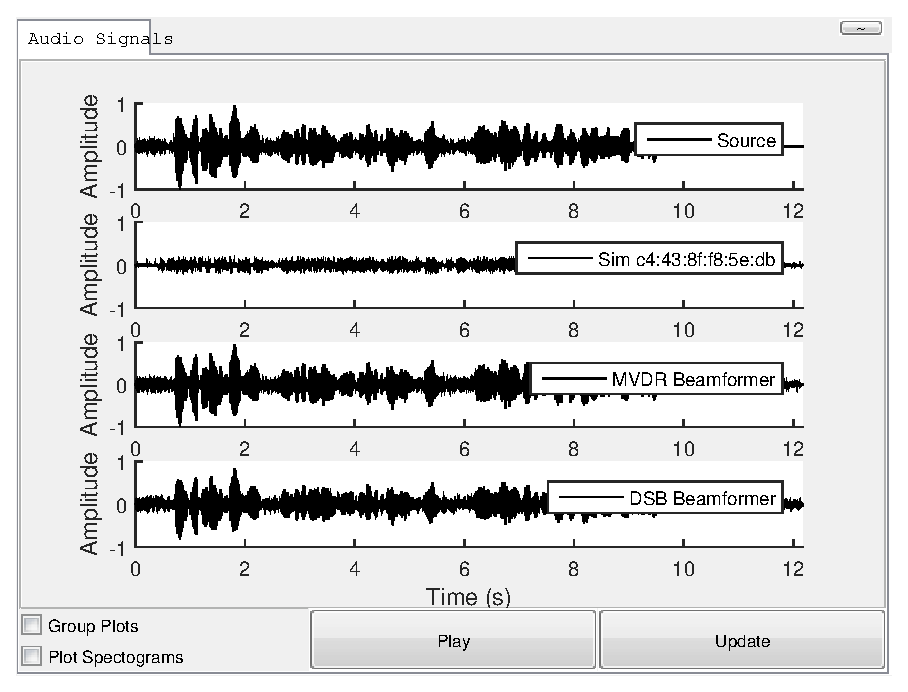
\includegraphics[scale = 0.9] {Screenshots_simulatie/Audio_signals/Signals_sim1} % l b r t]
	\caption[Audio signals simulation 1]{Audio signals simulation 1: Without reverberations, White noise added at 60dB SNR, without position errors} 
	\label{fig:Asim1}
\end{figure}

\begin{figure}[b!]
	\centering  
	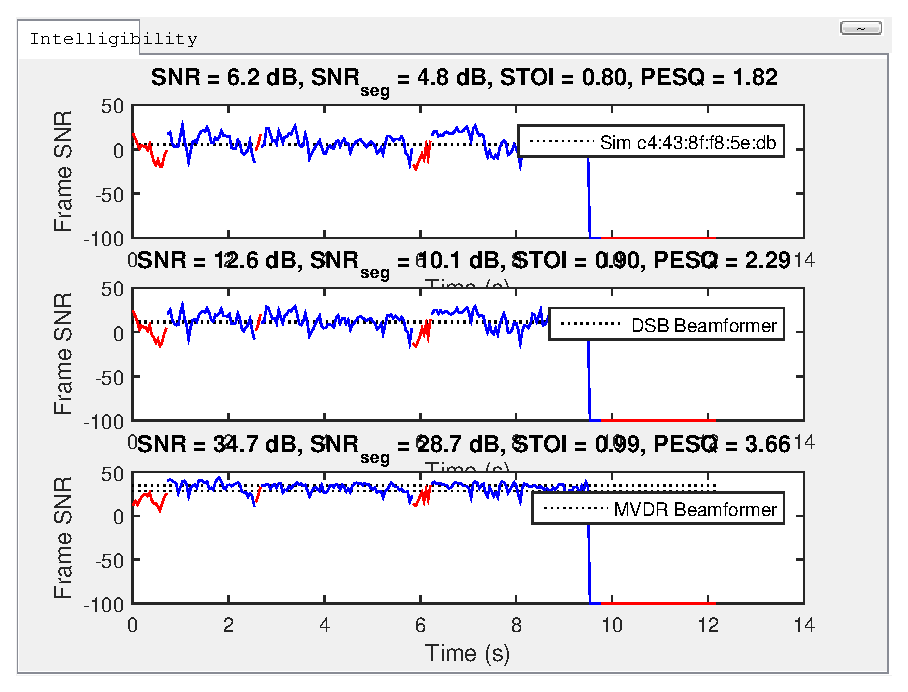
\includegraphics[scale = 0.9] {Screenshots_simulatie/Intelligibility/Simulatie1} % l b r t]
	\caption[Intelligibility simulation 1]{Intelligibility simulation 1: Without reverberations, White noise added at 60dB SNR, without position errors} 
	\label{fig:Isim1}
\end{figure}
\FloatBarrier
\subsection{Simulation 2}
\label{app:sim2}

\begin{figure}[h!]
	\centering  
	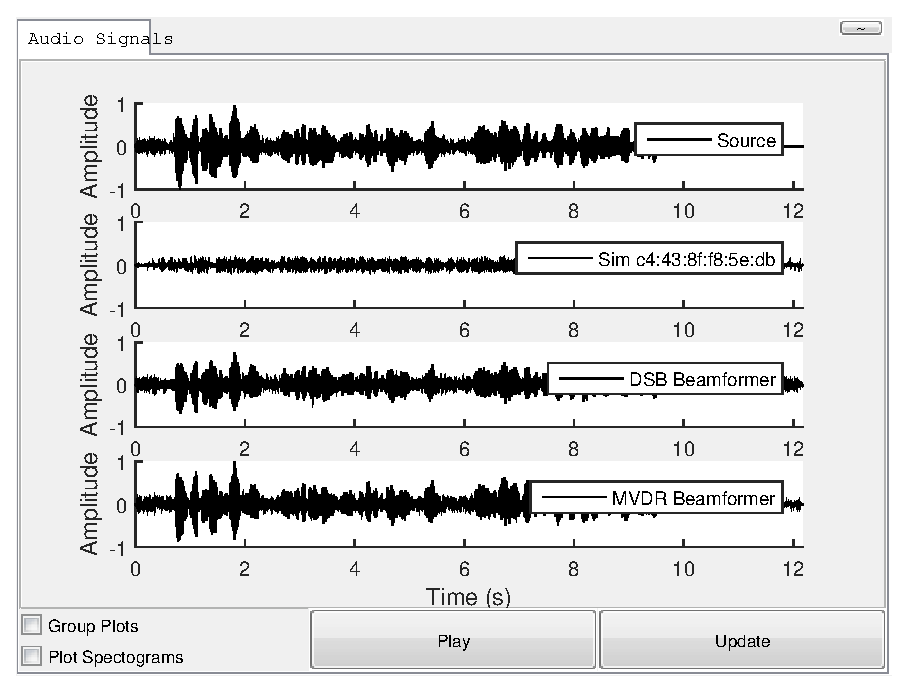
\includegraphics[scale = 0.9] {Screenshots_simulatie/Audio_signals/Signals_sim2} % l b r t]
	\caption[Audio signals simulation 2]{Audio signals simulation 2: With reverberations, White noise added at 60dB SNR, without position errors} 
	\label{fig:Asim2}
\end{figure}

\begin{figure}[b!]
	\centering  
	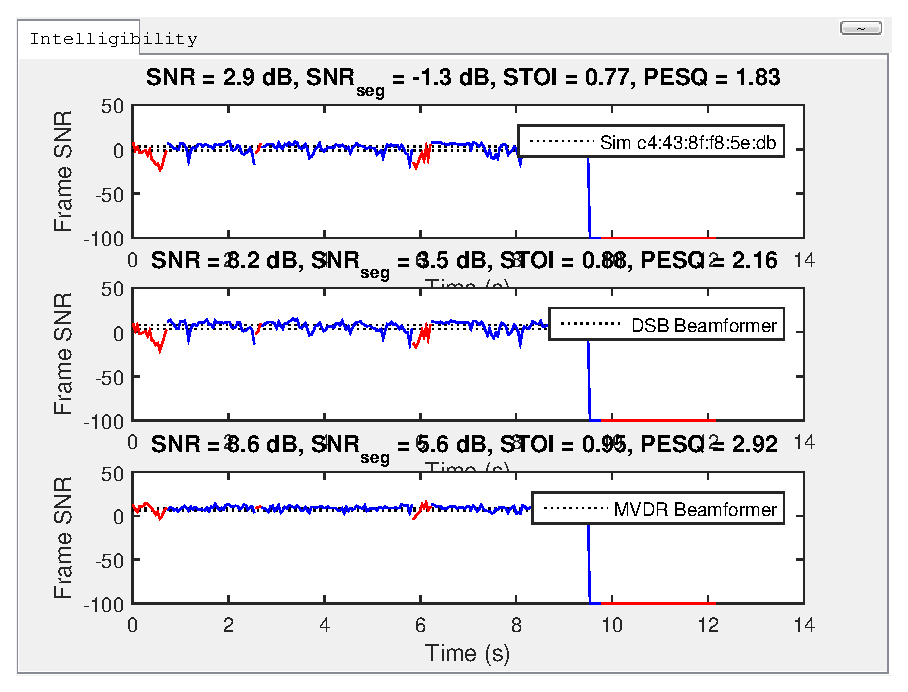
\includegraphics[scale = 0.9] {Screenshots_simulatie/Intelligibility/Simulatie2} % l b r t]
	\caption[Intelligibility simulation 2]{Intelligibility simulation 2: With reverberations, White noise added at 60dB SNR, without position errors} 
	\label{fig:Isim2}
\end{figure}
\FloatBarrier
\subsection{Simulation 3}
\label{app:sim3}

\begin{figure}[h!]
	\centering  
	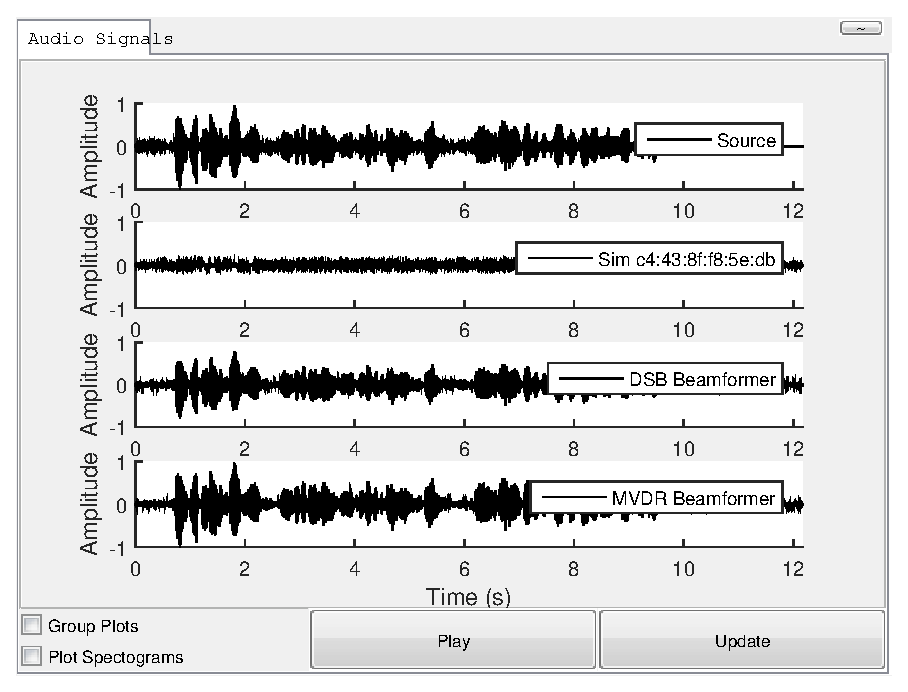
\includegraphics[scale = 0.9] {Screenshots_simulatie/Audio_signals/Signals_sim3} % l b r t]
	\caption[Audio signals simulation 3]{Audio signals simulation 3: Without reverberations, White noise added at 40dB SNR, without position errors} 
	\label{fig:Asim3}
\end{figure}

\begin{figure}[b!]
	\centering  
	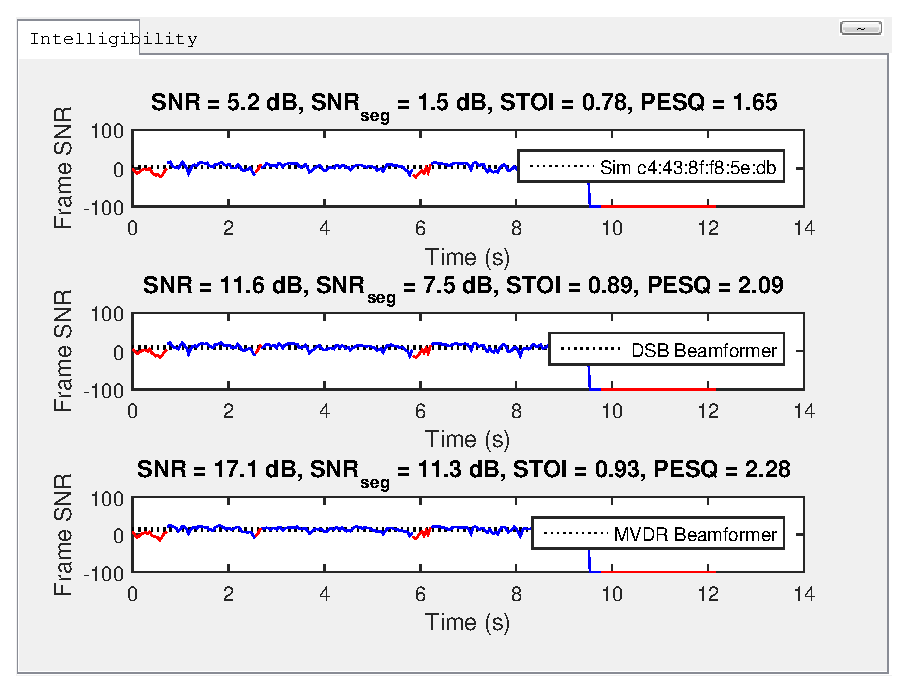
\includegraphics[scale = 0.9] {Screenshots_simulatie/Intelligibility/Simulatie3} % l b r t]
	\caption[Intelligibility simulation 3]{Intelligibility simulation 3: Without reverberations, White noise added at 40dB SNR, without position errors} 
	\label{fig:Isim3}
\end{figure}
\FloatBarrier
\subsection{Simulation 4}
\label{app:sim4}

\begin{figure}[h!]
	\centering  
	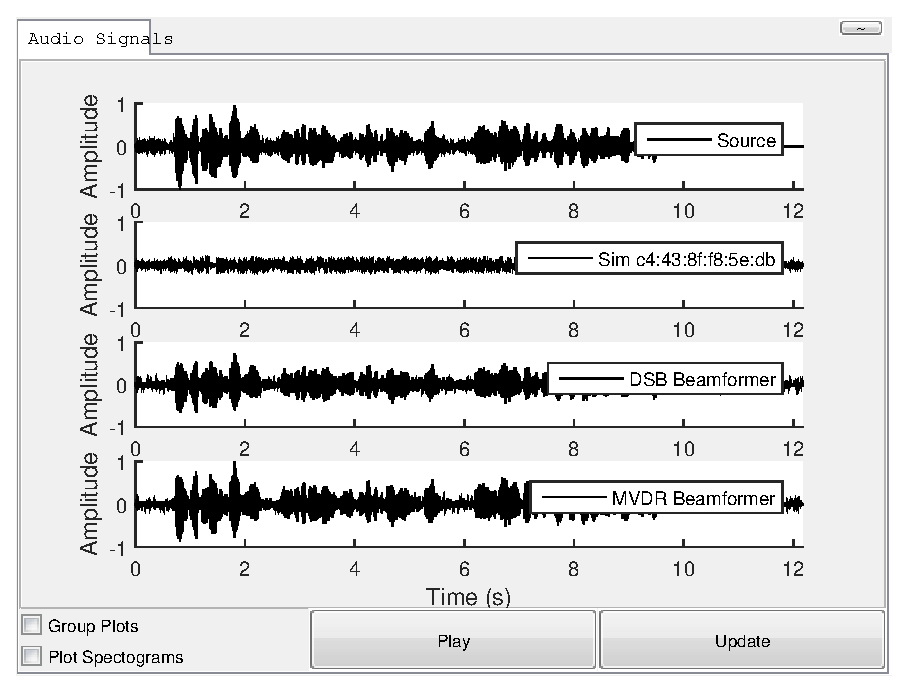
\includegraphics[scale = 0.9] {Screenshots_simulatie/Audio_signals/Signals_sim4} % l b r t]
	\caption[Audio signals simulation 4]{Audio signals simulation 4: Without reverberations, White noise added at 40dB SNR, without position errors} 
	\label{fig:Asim4}
\end{figure}

\begin{figure}[b!]
	\centering  
	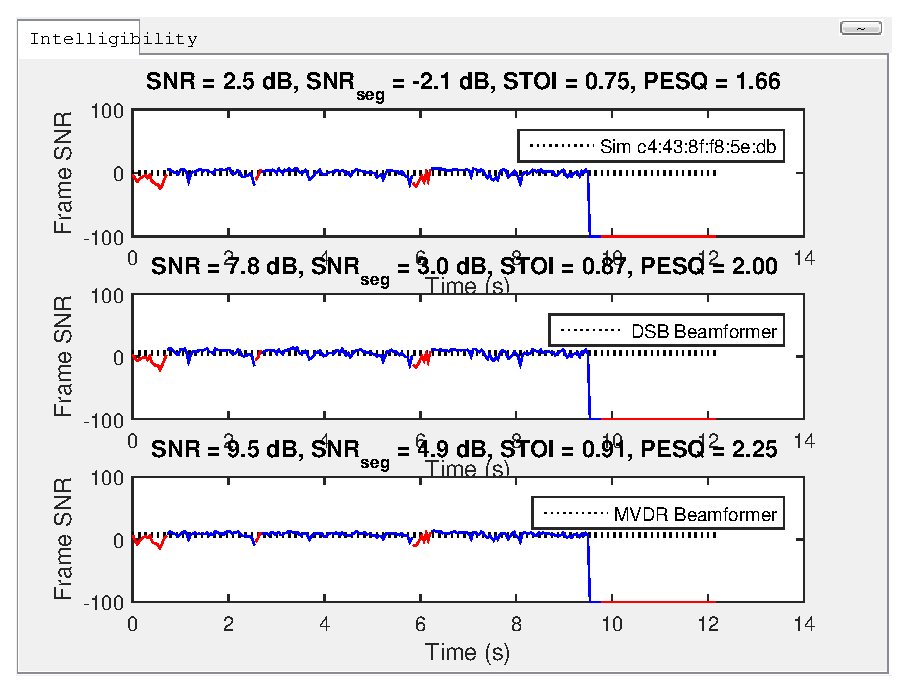
\includegraphics[scale = 0.9] {Screenshots_simulatie/Intelligibility/Simulatie4} % l b r t]
	\caption[Intelligibility simulation 4]{Intelligibility simulation 4: Without reverberations, White noise added at 40dB SNR, without position errors} 
	\label{fig:Isim4}
\end{figure}
\FloatBarrier
%\subsection{Simulation 5}
%\label{app:sim5}
%
%\begin{figure}[h!]
%	\centering  
%	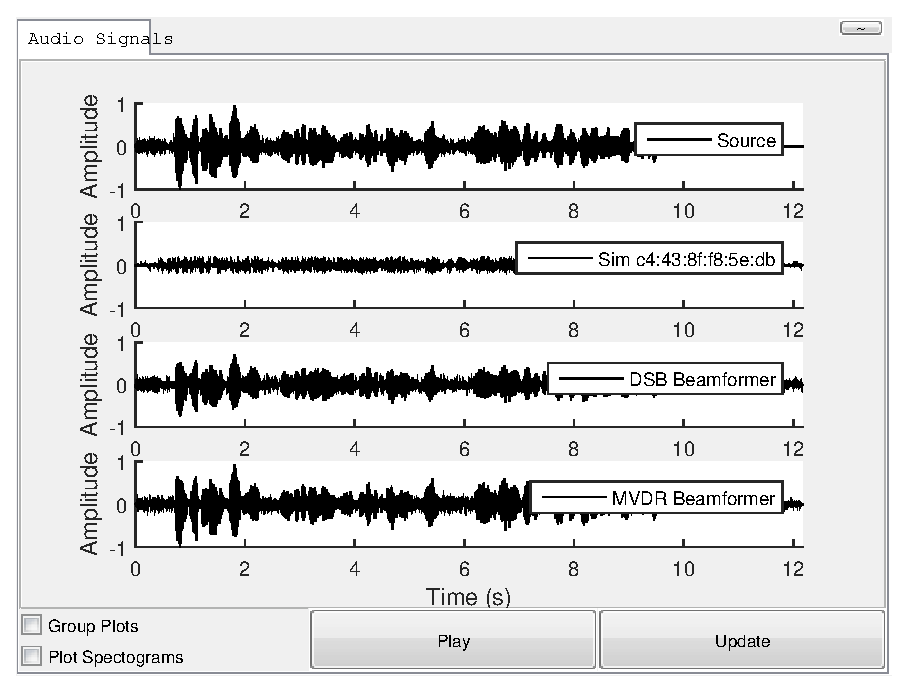
\includegraphics[scale = 0.9] {Screenshots_simulatie/Audio_signals/Signals_sim5} % l b r t]
%	\caption[Audio signals simulation 5: Without reverberations, White noise added at 60dB SNR, with position errors with a standard deviation of $0.05 cm$]{Audio signals simulation 5: Without reverberations, White noise added at 60dB SNR, with position errors with a standard deviation of $0.05 cm$} 
%	\label{fig:Asim5}
%\end{figure}
%
%\begin{figure}[b!]
%	\centering  
%	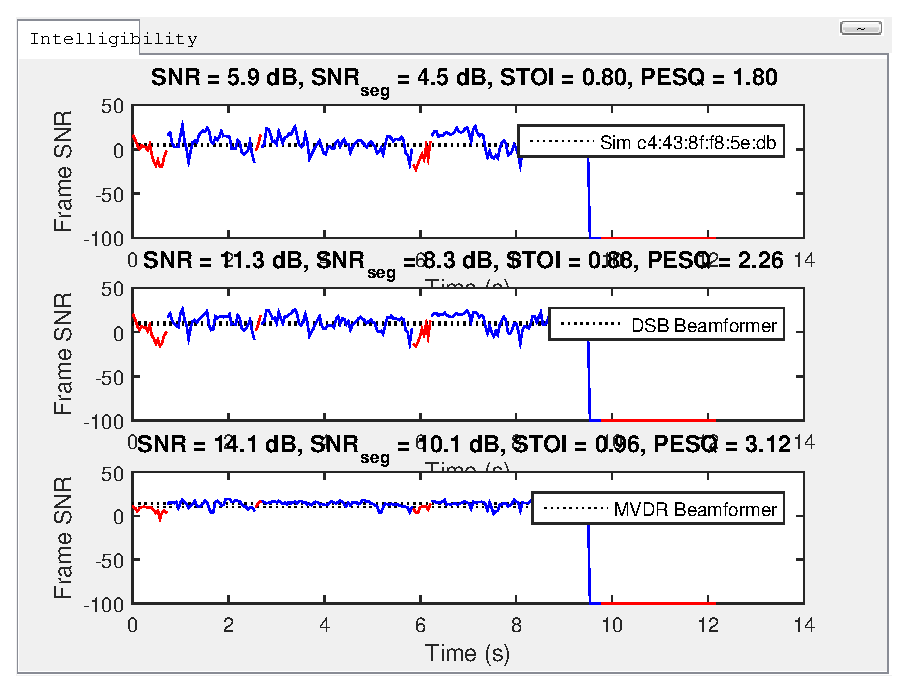
\includegraphics[scale = 0.9] {Screenshots_simulatie/Intelligibility/Simulatie5} % l b r t]
%	\caption[Intelligibility simulation 5: Without reverberations, White noise added at 60dB SNR, with position errors with a standard deviation of $0.05 cm$]{Intelligibility simulation 5: Without reverberations, White noise added at 60dB SNR, with position errors with a standard deviation of $0.05 cm$} 
%	\label{fig:Isim5}
%\end{figure}

\subsection{Simulation 6}
\label{app:sim6}

\begin{figure}[h!]
	\centering  
	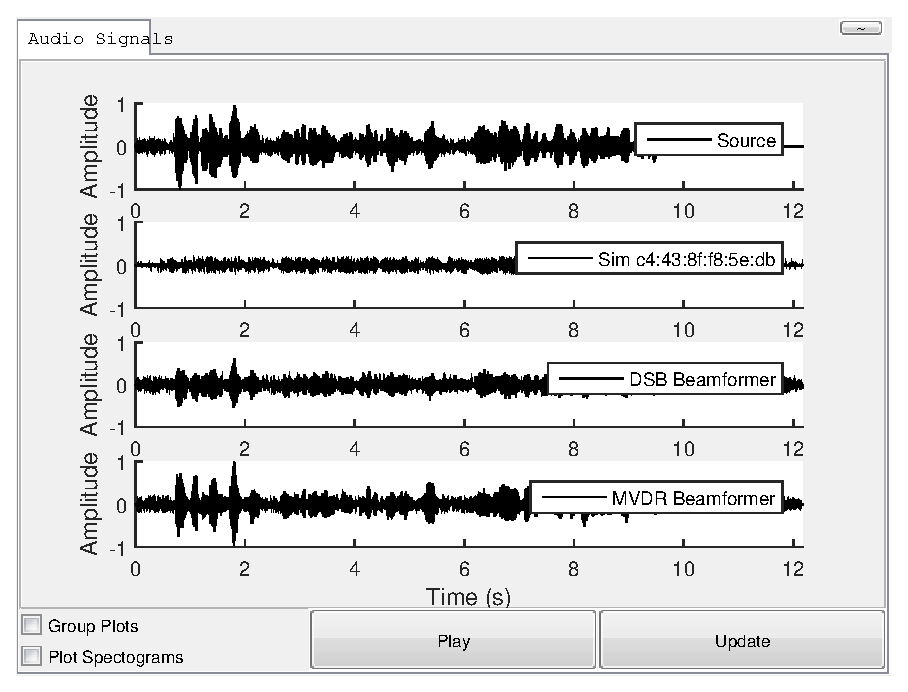
\includegraphics[scale = 0.88] {Screenshots_simulatie/Audio_signals/Signals_sim6} % l b r t]
	\caption[Audio signals simulation 6]{Audio signals simulation 6: With reverberations, White noise added at 60dB SNR, with position errors with a sigma of $0.05 cm$} 
	\label{fig:Asim6}
\end{figure}

\begin{figure}[b!]
	\centering  
	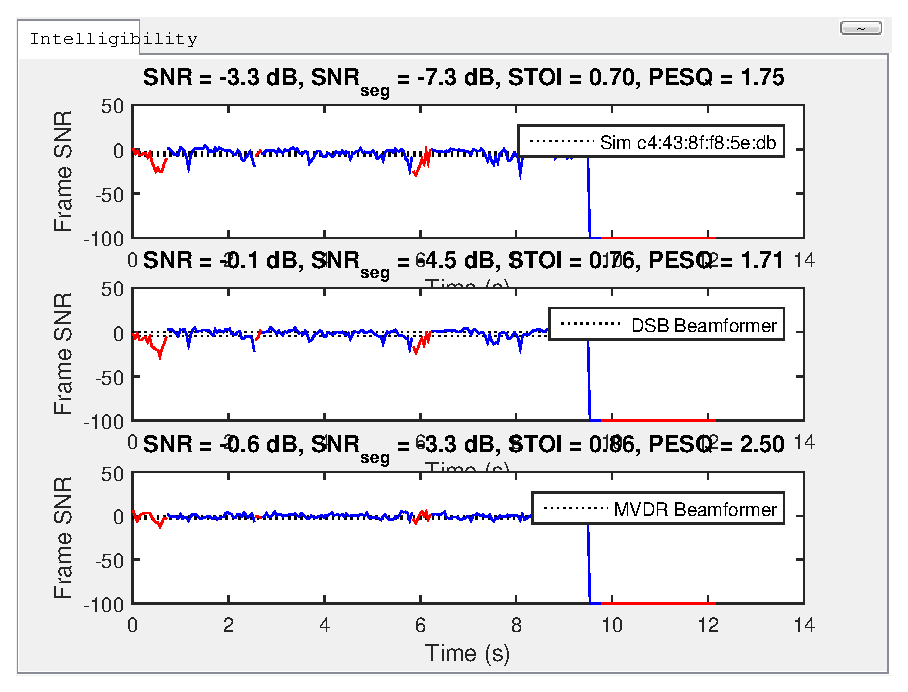
\includegraphics[scale = 0.88] {Screenshots_simulatie/Intelligibility/Simulatie6} % l b r t]
	\caption[Intelligibility simulation 6]{Intelligibility simulation 6: With reverberations, White noise added at 60dB SNR, with position errors with a sigma of $0.05 cm$} 
	\label{fig:Isim6}
\end{figure}
\FloatBarrier
\section{Office room experiments}
\label{app:room}
\FloatBarrier

\subsection{Office room experiment 1}
\label{app:room1}

\begin{figure}[h!]
	\centering  
	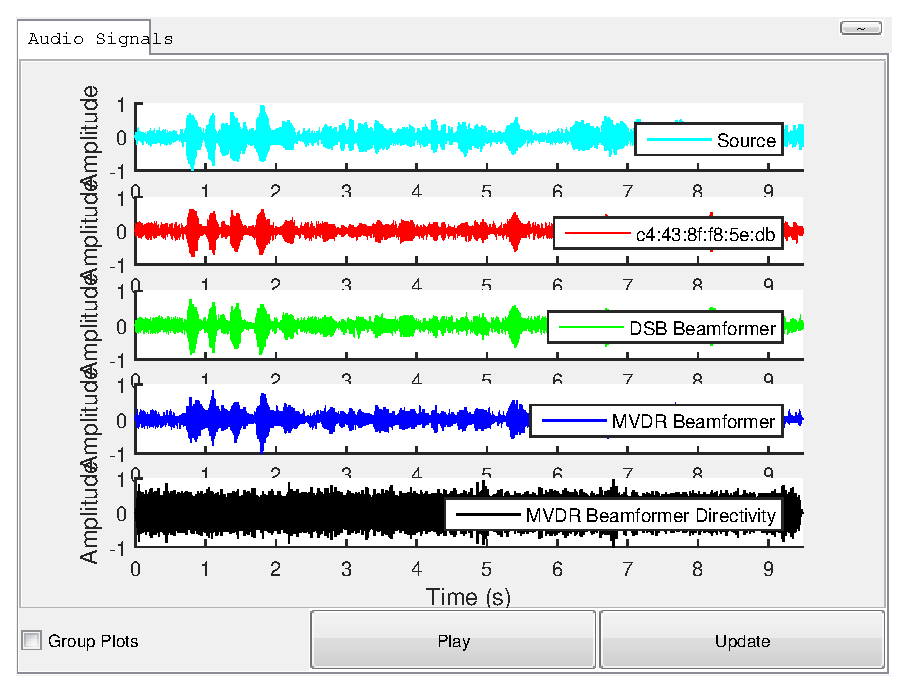
\includegraphics[scale = 0.88] {Screenshots_experimenten/Audio_signals/signals_18u36} % l b r t]
	\caption[Audio signals office room experiment 1]{Audio signals office room experiment 1: With an interfering audio source, $\theta = -90\degree$} 
	\label{fig:Aroom1}
\end{figure}

\begin{figure}[b!]
	\centering  
	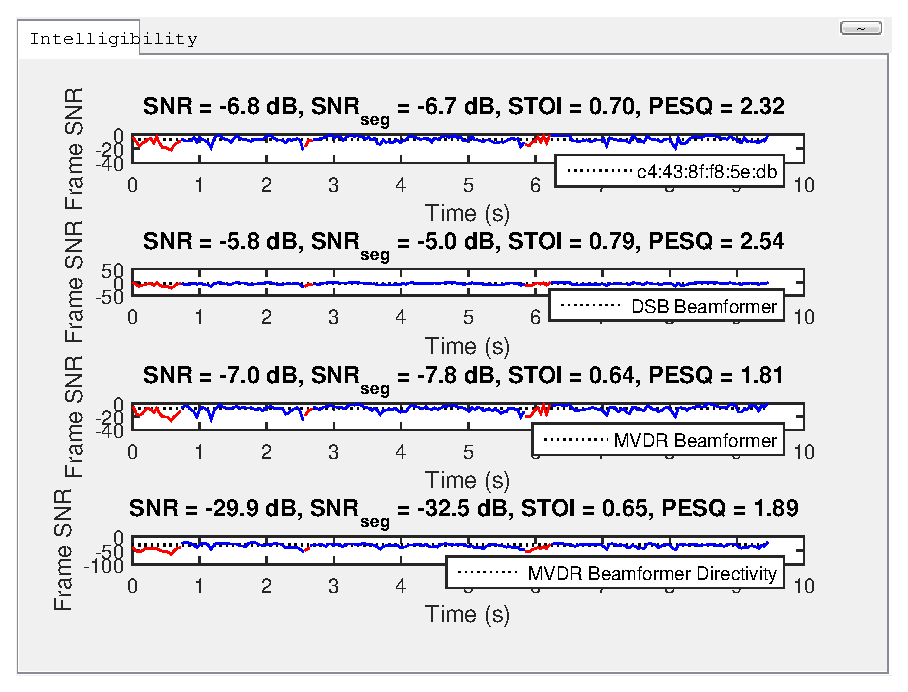
\includegraphics[scale = 0.88] {Screenshots_experimenten/Intelligibility/Intelligibility_18u36} % l b r t]
	\caption[Intelligibility office room experiment 1]{Intelligibility office room experiment 1: With an interfering audio source, $\theta = -90\degree$} 
	\label{fig:Iroom1}
\end{figure}

\FloatBarrier

\subsection{Office room experiment 2}
\label{app:room2}

\begin{figure}[h!]
	\centering  
	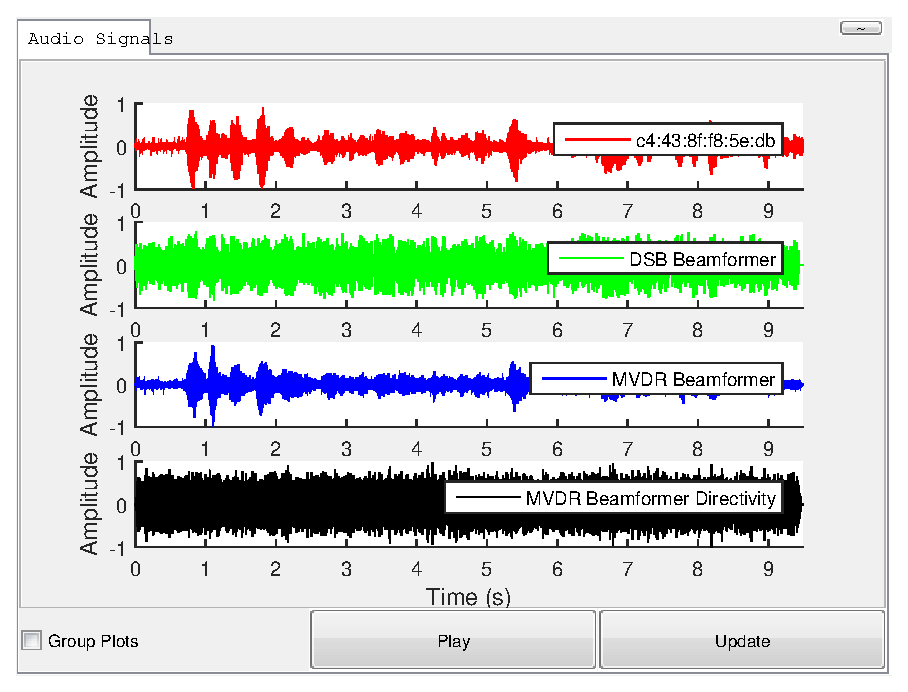
\includegraphics[scale = 0.9] {Screenshots_experimenten/Audio_signals/signals_20u21} % l b r t]
	\caption[Audio signals office room experiment 2]{Audio signals office room experiment 2: With an interfering audio source, $\theta = 0\degree$} 
	\label{fig:Aroom2}
\end{figure}

\begin{figure}[b!]
	\centering  
	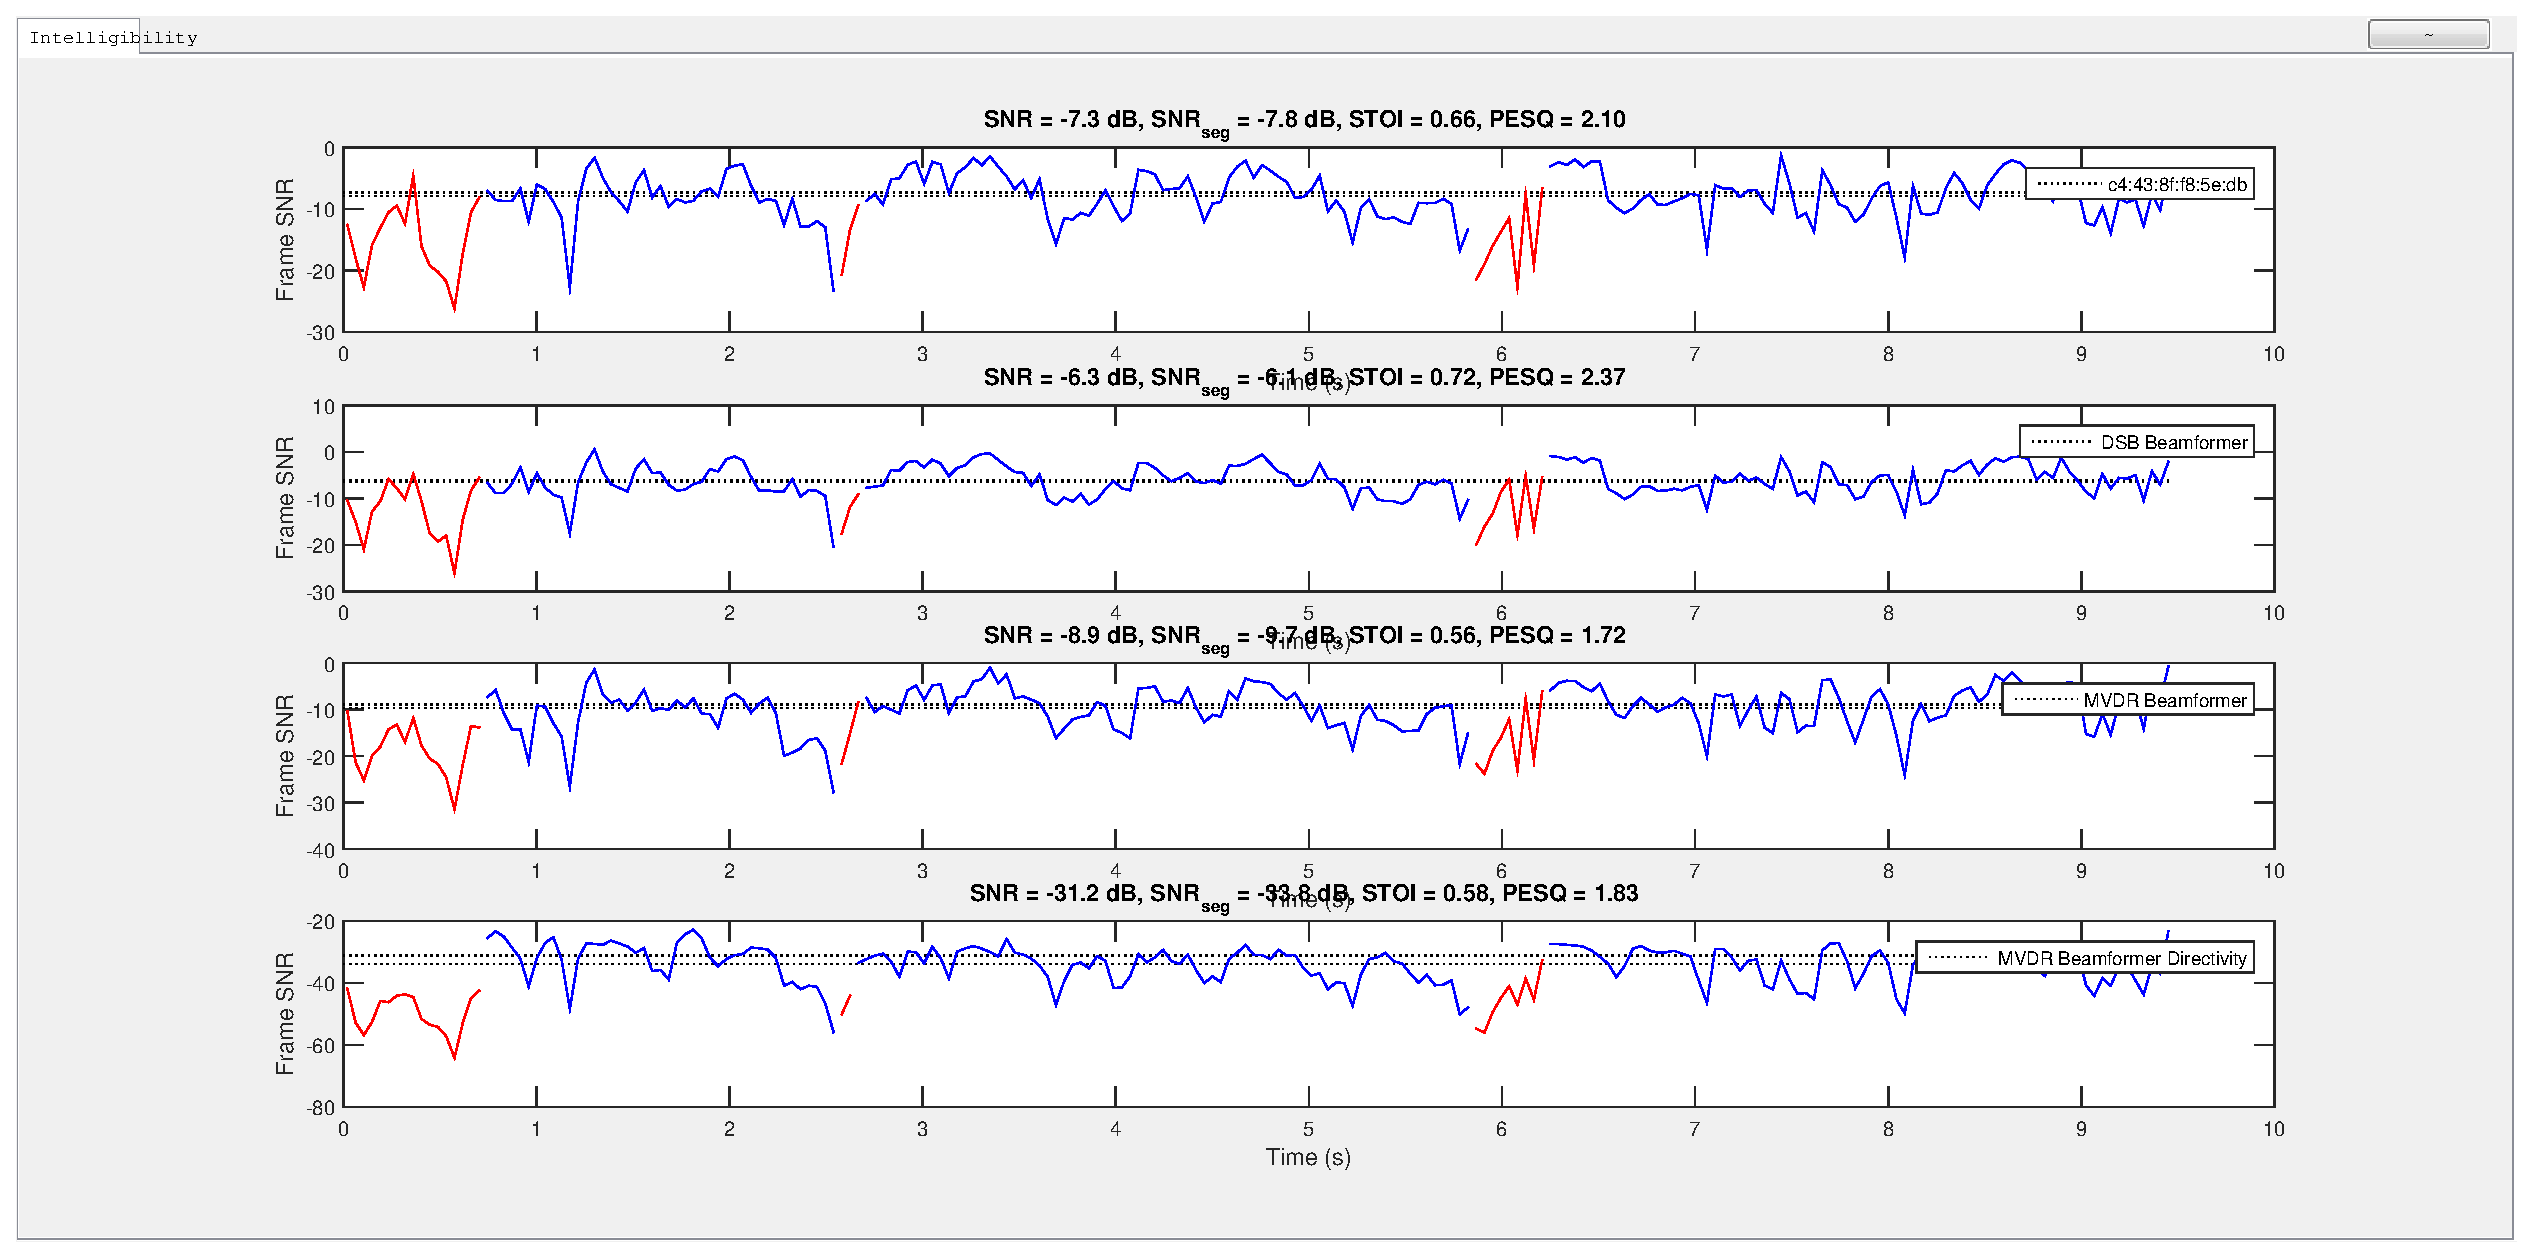
\includegraphics[width = \columnwidth] {Screenshots_experimenten/Intelligibility/Intelligibility_20u21} % l b r t]
	\caption[Intelligibility office room experiment 2]{Intelligibility office room experiment 2: With an interfering audio source, $\theta = 0\degree$} 
	\label{fig:Iroom2}
\end{figure}

\FloatBarrier

\subsection{Office room experiment 3}
\label{app:room3}

\begin{figure}[h!]
	\centering  
	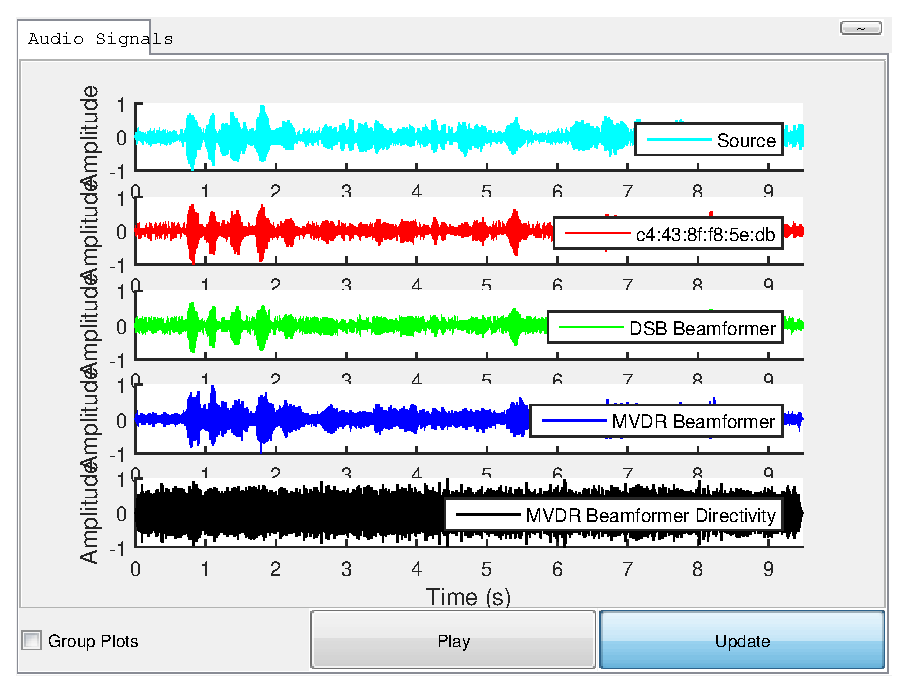
\includegraphics[scale = 0.9] {Screenshots_experimenten/Audio_signals/signals_20u29} % l b r t]
	\caption[Audio signals office room experiment 3]{Audio signals office room experiment 3: With an interfering audio source, $\theta = 90\degree$} 
	\label{fig:Aroom3}
\end{figure}

\begin{figure}[b!]
	\centering  
	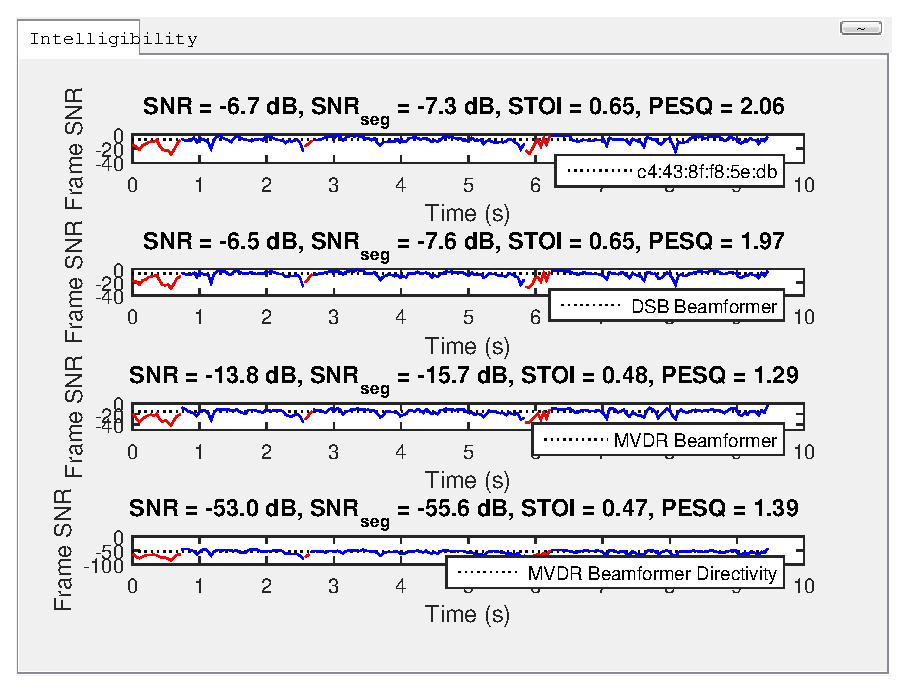
\includegraphics[scale = 0.9] {Screenshots_experimenten/Intelligibility/Intelligibility_20u39} % l b r t]
	\caption[Intelligibility office room experiment 3]{Intelligibility office room experiment 3: With an interfering audio source, $\theta = 90\degree$} 
	\label{fig:Iroom3}
\end{figure}

\FloatBarrier

\subsection{Office room experiment 4}
\label{app:room4}

\begin{figure}[h!]
	\centering  
	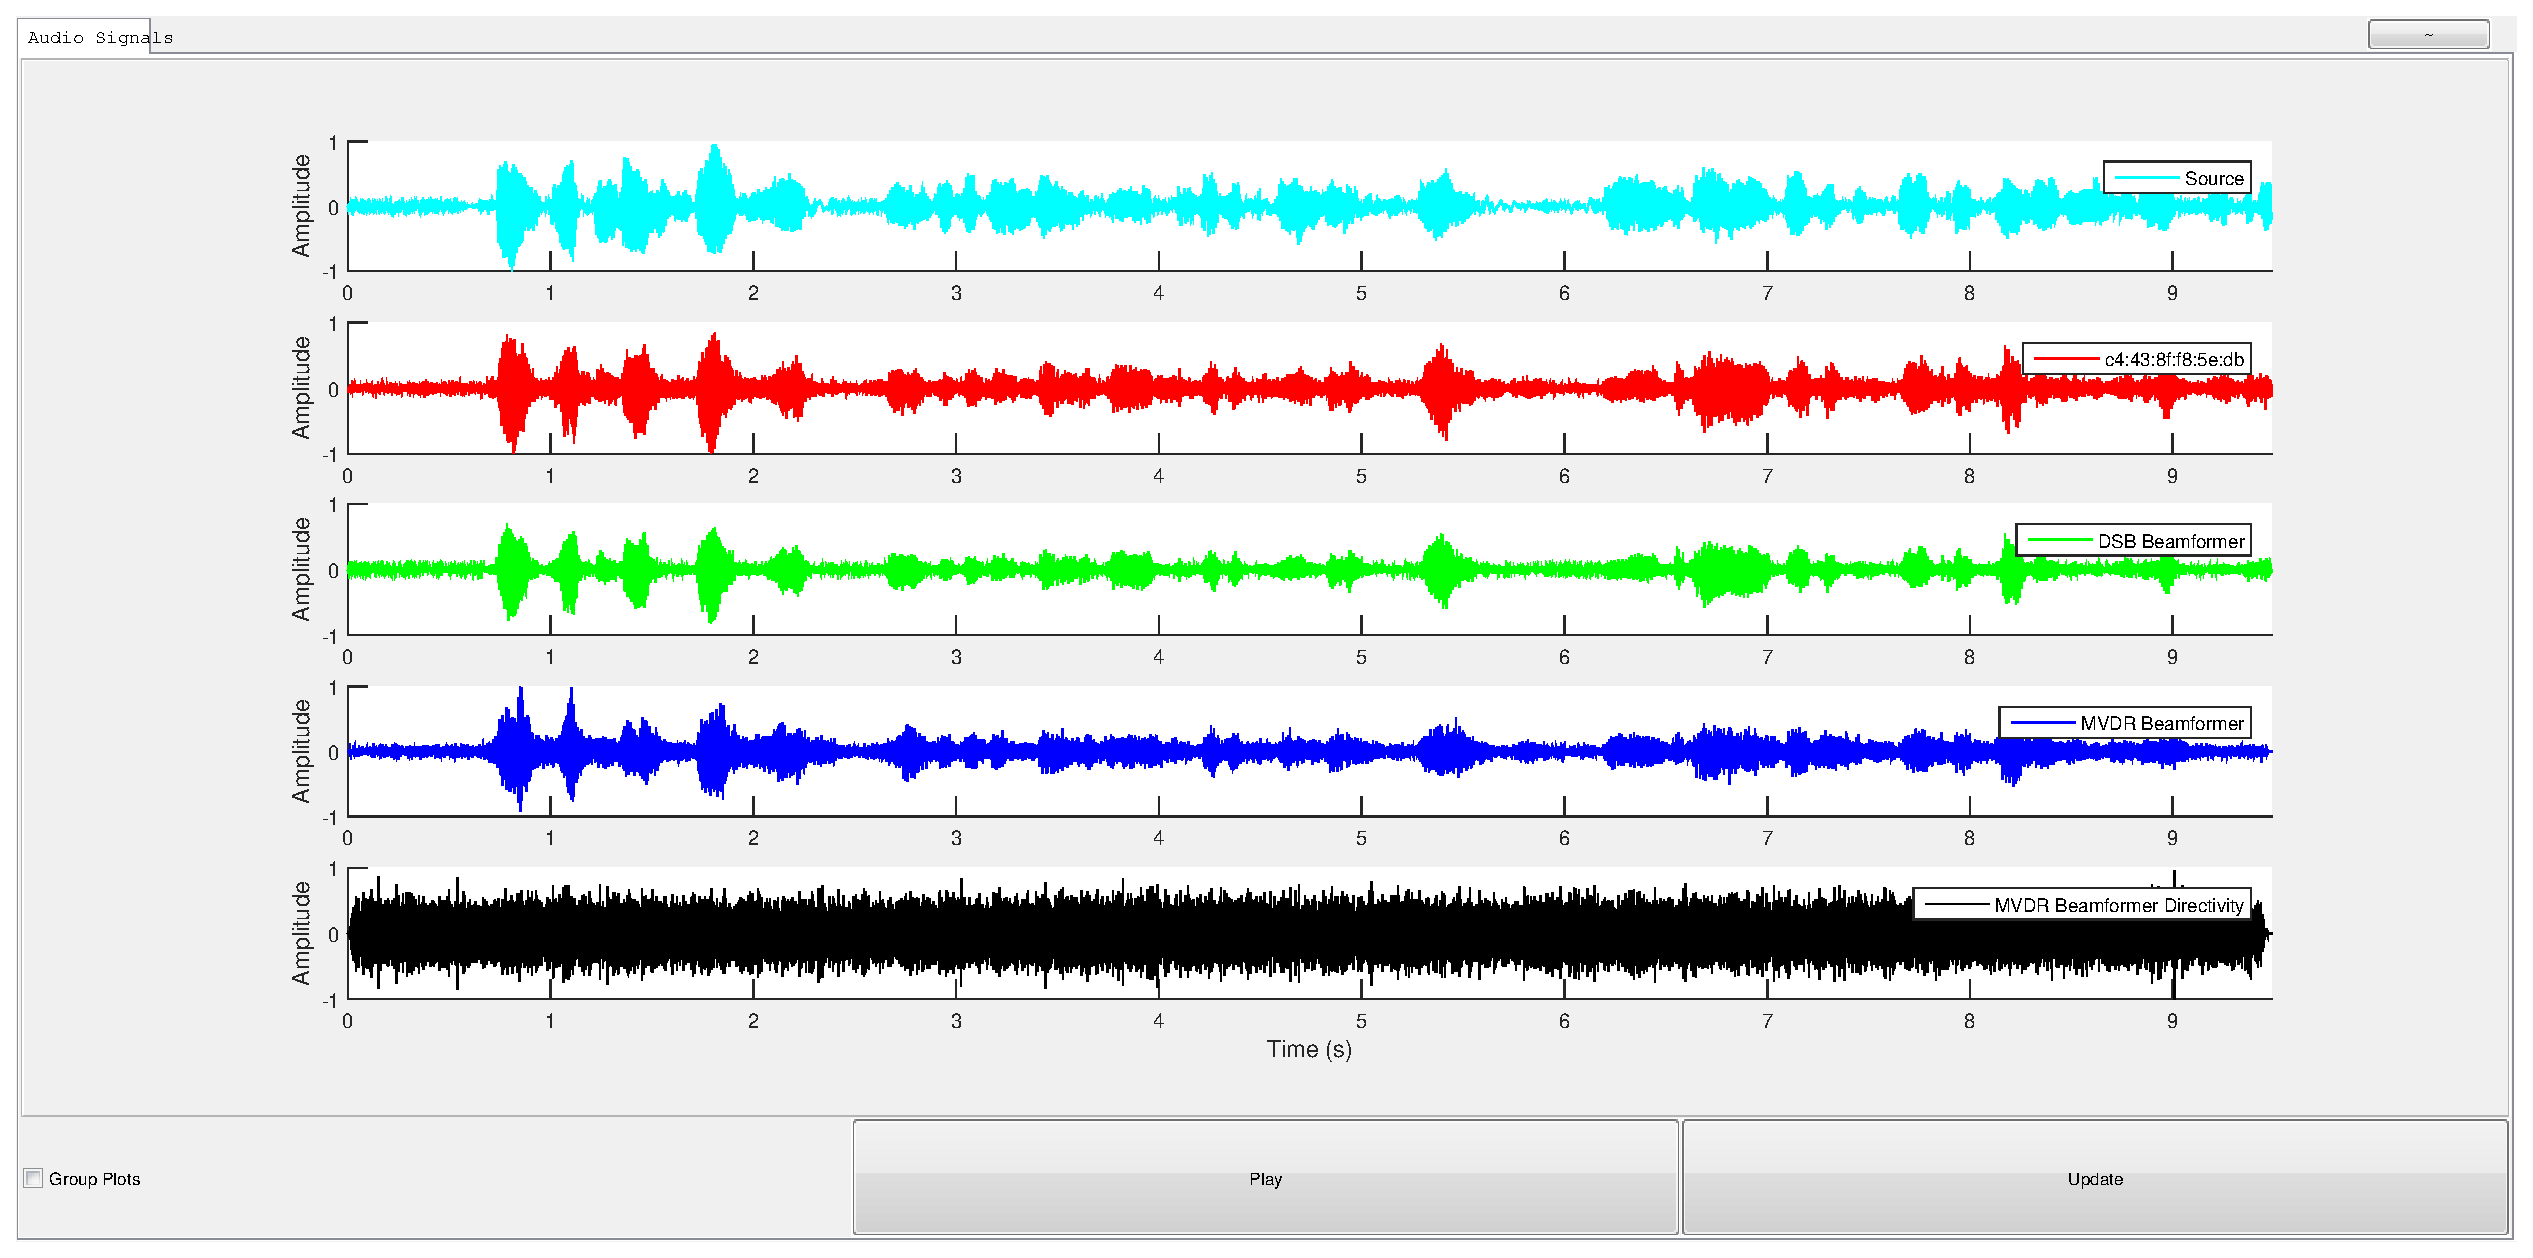
\includegraphics[width = \columnwidth] {Screenshots_experimenten/Audio_signals/signals_20u55} % l b r t]
	\caption[Audio signals office room experiment 4]{Audio signals office room experiment 4: With an interfering audio source, Different orientations} 
	\label{fig:Aroom4}
\end{figure}

\begin{figure}[b!]
	\centering  
	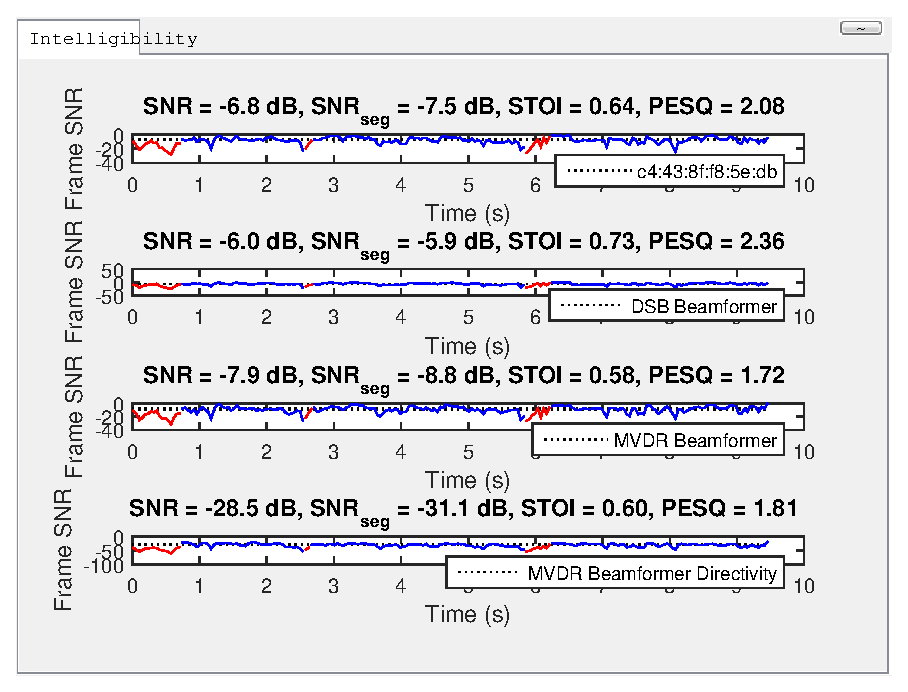
\includegraphics[scale = 0.9] {Screenshots_experimenten/Intelligibility/Intelligibility_20u55} % l b r t]
	\caption[Intelligibility office room experiment 4]{Intelligibility office room experiment 4: With an interfering audio source, Different orientations} 
	\label{fig:Iroom4}
\end{figure}

\FloatBarrier

\subsection{Office room experiment 5}
\label{app:room5}

\begin{figure}[h!]
	\centering  
	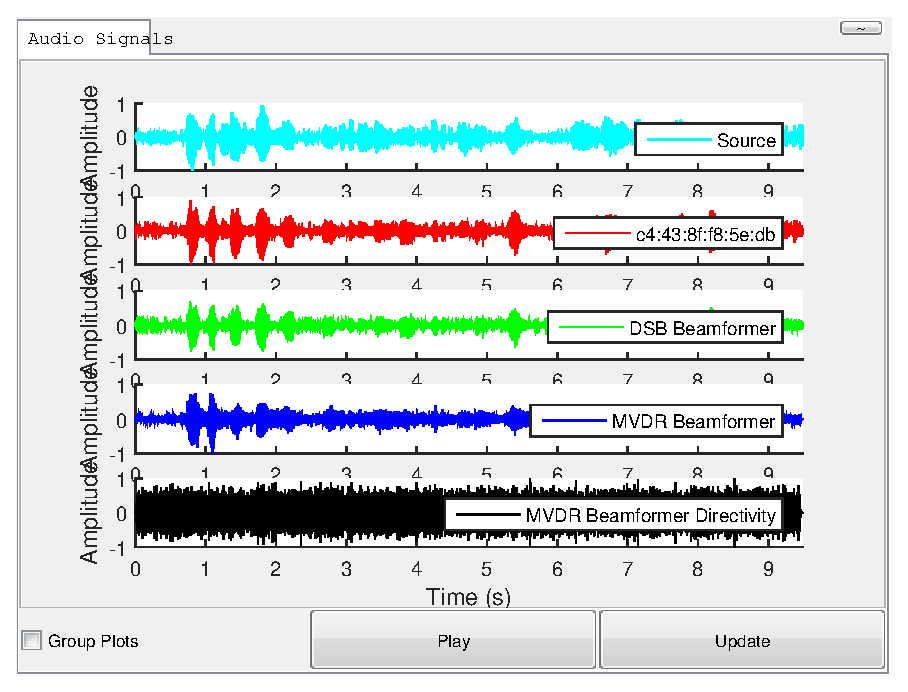
\includegraphics[scale = 0.9] {Screenshots_experimenten/Audio_signals/signals_21u07} % l b r t]
	\caption[Audio signals office room experiment 5]{Audio signals office room experiment 5: With an interfering audio source, Linear array} 
	\label{fig:Aroom5}
\end{figure}

\begin{figure}[b!]
	\centering  
	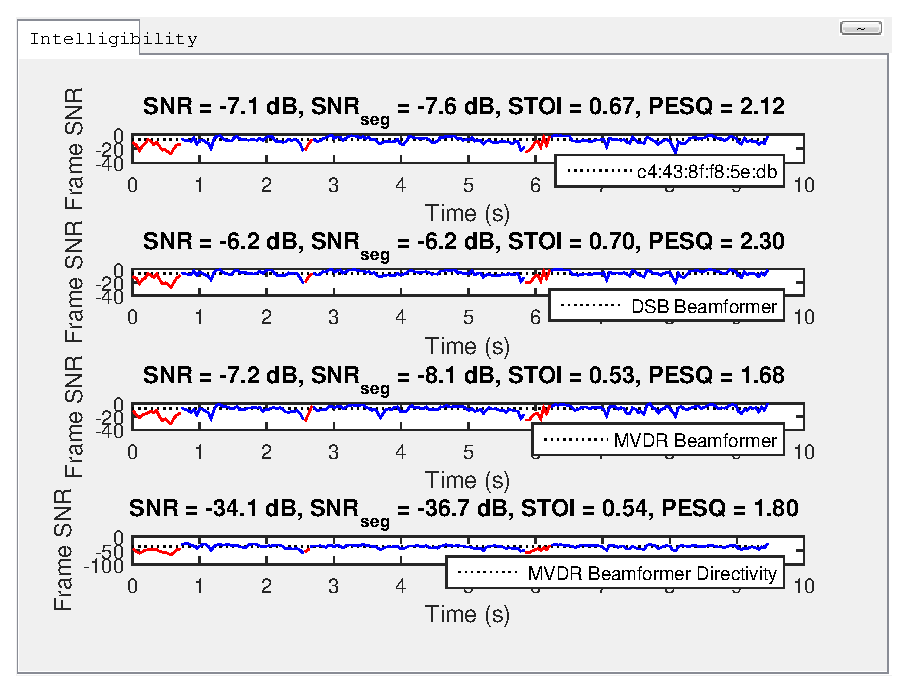
\includegraphics[scale = 0.9] {Screenshots_experimenten/Intelligibility/Intelligibility_21u07} % l b r t]
	\caption[Intelligibility office room experiment 5]{Intelligibility office room experiment 5: With an interfering audio source, Linear array} 
	\label{fig:Iroom5}
\end{figure}

\FloatBarrier

\section{Anechoic chamber experiments}
\label{app:anechoic}

\subsection{Anechoic chamber experiment 1}
\label{app:anechoic1}

\FloatBarrier

\begin{figure}[h!]
	\centering  
	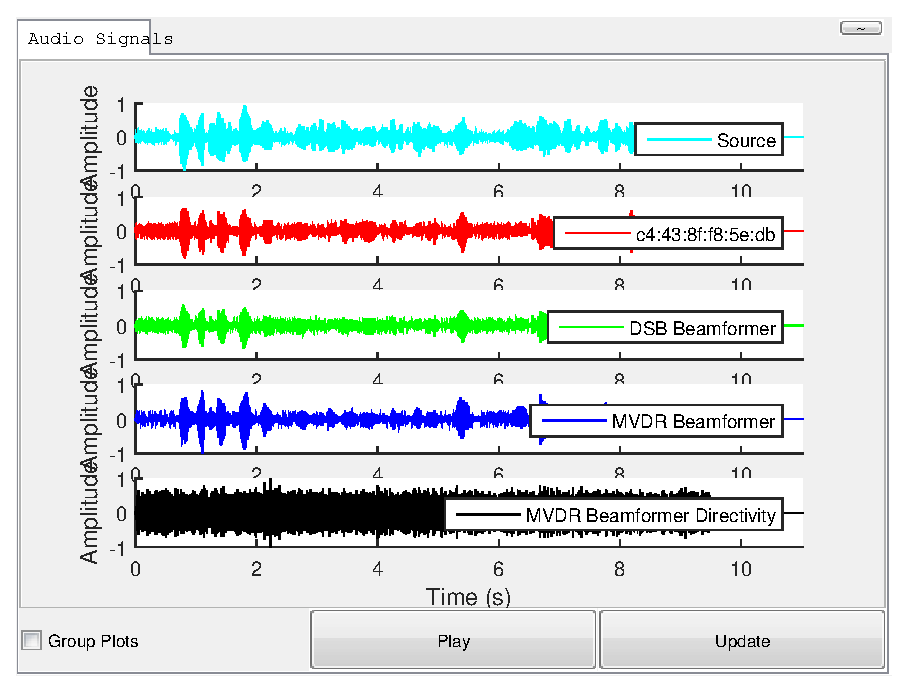
\includegraphics[scale = 0.85] {Screenshots_experimenten/Audio_signals/signals_18u27} % l b r t]
	\caption[Audio signals anechoic chamber experiment 1]{Audio signals anechoic chamber experiment 1: With an interfering audio source} 
	\label{fig:Aanechoic1}
\end{figure}

\begin{figure}[b!]
	\centering  
	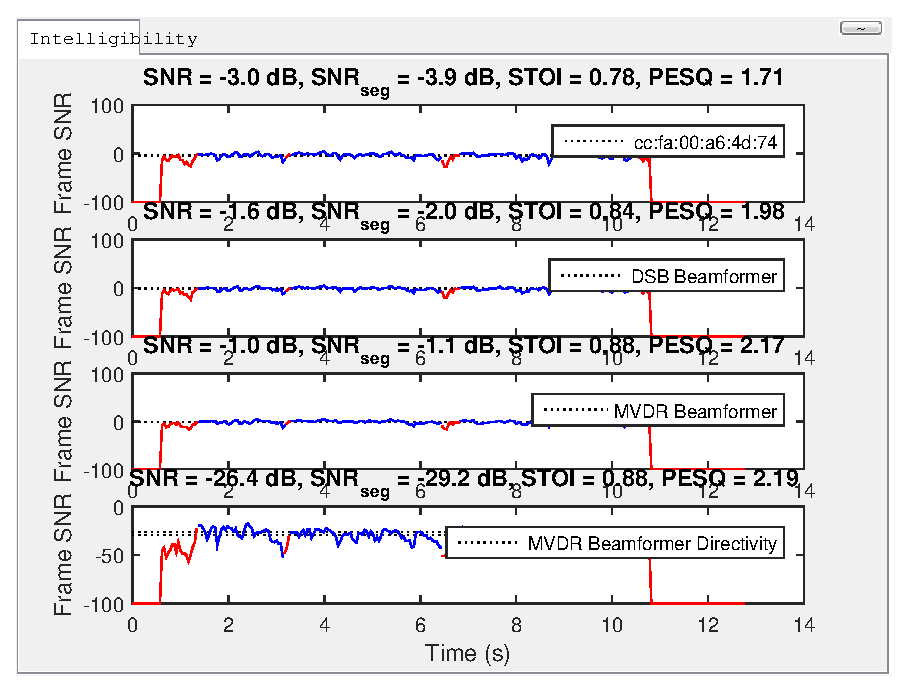
\includegraphics[scale = 0.85] {Screenshots_experimenten/Intelligibility/anechoic} % l b r t]
	\caption[Intelligibility anechoic chamber experiment 1]{Intelligibility anechoic chamber experiment 1: With an interfering audio source} 
	\label{fig:Ianechoic1}
\end{figure}

\FloatBarrier

\bibliography{bibliography}

\end{document}